\documentclass[11pt,a4paper]{article}

% --- 1. Encoding, Fonts, Language ---
\usepackage[utf8]{inputenc}
\usepackage[T1]{fontenc}
\usepackage{lmodern}
\usepackage[english]{babel}

% --- 2. Mathematics ---
\usepackage{amsmath, amssymb, amsthm}
\usepackage{empheq}

% --- Theorem environments (manual numbering kept consistent with cross-references) ---
\theoremstyle{plain}
\newtheorem*{thmA}{Theorem 1 (Exclusion of the static lattice)}
\newtheorem*{thmB}{Theorem 2 (Exclusion of the self-bound liquid)}
\newtheorem*{thmC}{Theorem 3 (Exact covariance of the scalar sector)}
\newtheorem*{thmD}{Theorem 4 (Uniqueness of the Johns node from substrate constraints)}
\theoremstyle{remark}
\newtheorem*{remarkstar}{Remark}

% --- 3. Geometry and Layout ---
\usepackage[margin=2.5cm]{geometry}
\usepackage{titlesec}
\usepackage{enumitem}

% --- 4. Tables, Figures, Captions ---
\usepackage{graphicx}
\graphicspath{{../figures/}}
\usepackage{booktabs}
\usepackage{longtable}
\usepackage{array}
\usepackage{caption}

% --- 5. TikZ (2D & 3D) ---
\usepackage{tikz}
\usepackage{tikz-3dplot}
\usetikzlibrary{arrows.meta, backgrounds, shadings, positioning, calc}

\tikzset{
    picto_box/.style={
        draw=gray!60,
        thick,
        minimum width=1.5cm,
        minimum height=1.5cm,
        inner sep=5pt,
        rounded corners=2pt
    },
    pole/.style={circle, fill=black, inner sep=1.2pt}
}

% --- 6. Hyperlinks (always load last!) ---
\usepackage{hyperref}
\hypersetup{
    colorlinks=true,
    linkcolor=blue,
    urlcolor=cyan,
    pdftitle={Dipolar String Model: an Exploratory Framework for the Vacuum from Transmission-Line Electrodynamics},
}

% --- 7. Document metadata ---
\title{\textbf{Dipolar String Model:}\\ \large an Exploratory Framework for the Vacuum from Transmission-Line Electrodynamics}
\author{R. St-Pierre\thanks{Independent researcher, Qu\'ebec, Canada. This research received no external funding. The author declares no conflict of interest.}}
\date{August 2026 --- admin@dipolarstrings.org --- V2.9.1 (Zenodo edition)}

% --- 8. Custom macros ---
\newcommand{\dqd}{\ensuremath{\ooalign{$\bigcirc$\cr\hfil\scalebox{0.7}{$=$}\hfil}}}
\newcommand{\Ncd}{\ensuremath{N_{\mathrm{DS}}}}

\begin{document}

\maketitle

\begin{abstract}
\noindent\textbf{Background.} We present the Dipolar Strings (DS) model, a deterministic phenomenological framework that treats the physical vacuum as a gas of massless dipolar cells --- Dipolar Quantum Doubles (DQD) --- modeled as impedance-matched bifilar transmission lines. The epistemological posture is explicit: General Relativity (GR) and Quantum Mechanics (QM) are taken as \emph{exact within their tested domains}; any divergence of the DS model from them in a tested regime is, by construction, a defect of the DS model. The model proposes a possible substrate beneath both theories, with Einsteinian geometry represented by the averaged elasticity of the medium and quantum kinematics explored through lattice phase dynamics. Its proper predictions live at the limits of the established theories, most concretely in the replacement of gravitational singularities by finite equilibria. The framework is a theory of the \emph{medium}, not of matter: the vacuum, light, and collective gravitation are in scope; the weak and strong sectors, neutrino masses, cosmological evolution, the Born rule, and a microscopic account of entanglement are not derived.

\noindent\textbf{Methods.} Electric charge is dictated topologically by the winding chirality of the closed loop (mirror senses carrying opposite signs); mass follows from closed-loop inductance. Gravity is treated as vacuum refraction driven by an impedance field $Z(\vec{x})$, governed by a scalar Lagrangian shown symbolically to be identically a field theory on the effective metric, with no explicit preferred-frame vector in the action. The interior of compact objects is obtained by numerical hydrostatic integration with the closure equation of state $u(\ell) = hc_0/\ell^4$, $P = u/3$.

\noindent\textbf{Results.} The framework yields the parameter-free geometric ratio $D/r = 2\cosh\pi$, while the calibrated electron aspect ratio gives $Z_e \simeq 0.73\,Z_0 \simeq 275~\Omega$ (robustly an impedance well, though its precise value rests on an underived aspect ratio, Section~\ref{sec:electron_impedance}); it further yields a scalar sector with first-post-Newtonian parameters $\gamma = \beta = 1$ (Section~\ref{sec:ppn}); and a stable branch of horizonless, singularity-free \emph{substrate stars} with critical mass $M_{\text{crit}} \approx 1.3\times10^{6}\,M_\odot \propto \ell_1^2$ and maximal compactness $r_s/R = 0.81$ (with the non-gravitating native energy $u_0$ of Axiom~A8 now consistently removed from the source, Section~\ref{sec:substrate_stars}). Because the tensor sector is driven to full General Relativity by the Deser bootstrap (Section~\ref{sec:tensor_sector}), the exterior of every compact object is Schwarzschild: the photon sphere sits at $3r_s/2$, configurations with $r_s/R > 2/3$ cast a shadow identical to that of a black hole, and no shadow-diameter, ISCO, or post-Newtonian deviation from GR is predicted (earlier statements of a $+4.63\,\%$ shadow deviation and of 2PN deviations are withdrawn as belonging to the scalar sector alone). The predicted median of the stable-branch mass distribution ($\log M = 6.02$) lies close to the median of the electron-scattering-corrected black-hole masses of the Little Red Dots ($\log M = 6.10$; Rusakov et al., Nature 2026); the earlier Kolmogorov--Smirnov statement is not re-evaluated on the corrected branch ($n = 7$; no discriminating power at this sample size). This channel is, however, now disfavoured: a direct dynamical mass measurement in a lensed little red dot returns $\approx 5\times10^{7}\,M_\odot$, consistent with the virial calibration and above the model's cutoff (Section~\ref{sec:lrd}). A time-stamped prediction of mass accumulation just below $M_{\text{crit}}$, testable on forthcoming JWST samples, is registered via a Zenodo deposit (Section~\ref{sec:lrd}). On the quantum side, Appendix~\ref{app:schrodinger} establishes on a surrogate Johns lattice that the envelope of a localized excitation obeys the free Schr\"odinger equation as its single-band quadratic truncation, with a single action quantum closing the de~Broglie relations and the inertial response.

\noindent\textbf{Conclusions.} The scalar gravitational sector is treated as a constrained (elliptic) mode --- the analogue of the Newtonian potential --- and reproduces General Relativity at first post-Newtonian order ($\gamma = \beta = 1$); it carries no radiation, so the absence of a breathing mode is an assumption of the construction rather than a derived prediction. After the tensor bootstrap the exterior is Schwarzschild and no post-Newtonian deviation of any order is predicted; the second-order deviations of the scalar sector alone ($\Delta g_{00} = -U^3/6$, $\Delta g_{ij} = +U^2\delta_{ij}/2$) are retained only as a diagnostic of an incomplete bootstrap. The preferred-frame parameters are not computed and are listed among the open problems. The registered mass-accumulation prediction is derived analytically as a caustic effect of the equilibrium branch and shown robust to the formation prior ($f_{1/2} \gtrsim 70\%$ for any smooth prior on the central density). All numerical results are reproduced by two independent implementations, and all codes and symbolic verifications are archived on Zenodo (concept DOI: 10.5281/zenodo.21196098). For the exploratory relation $G \stackrel{?}{=} (c_0^3\ell_1^2/2\pi\hbar)\,e^{-3/4\alpha}$, the telegrapher action conditionally yields the coefficient $3/4\alpha$ for a three-string fractional phase slip, but neither its scale/core contribution nor any mapping from phase-slip fugacity to $G$ is derived; the relation remains a conjecture ($-7.75\,\%$, exponent residual $0.0785\,\%$; Section~\ref{sec:g_closure}). The model is presented as a speculative working hypothesis whose falsification hierarchy is: (1)~the permanent absence of PBH evaporation bursts (binary outcome); (2)~non-periodic post-merger echoes at geometrically growing spacing from fresh remnants; (3)~the hard LRD mass cutoff and the $-1/2$ caustic exponent of the mass function (JWST; the accompanying thermal emission is a luminosity requirement whose spectral form awaits the two-component interior calculation, Section~\ref{sec:open_problems}); (4)~the absence of a breathing mode (LVK), stated at the level of an assumption of the construction; its principal open problems --- foremost the absence of a microscopic derivation of the medium --- are inventoried explicitly.

\medskip
\noindent\textbf{Keywords:} analogue gravity; transmission lines; vacuum impedance; polarizable vacuum; substrate stars; black hole mimickers; Little Red Dots; JWST; emergent Lorentz invariance.
\end{abstract}

\tableofcontents
\newpage

\section{Introduction}
The Dipolar Strings (DS) model proposes an elementary structure in the form of a string containing an energy fluid of fractional charge $e/3$, possessing an intrinsic negative pole and positive pole. We study the potential consequences of this object in a dynamical space through the approach of transmission lines, characteristic impedance, and Coulomb forces.

\subsection*{Epistemological positioning of the model}
This model adopts the posture of analogue models \cite{barcelo, volovik} toward General Relativity and Quantum Mechanics:
\begin{enumerate}[label=(\roman*)]
    \item GR and QM are taken as \textbf{exact within their domains}; any divergence of the DS model from them in a tested regime is a defect of the DS model, by construction.
    \item The DS model proposes the \textbf{common lower level}: a single medium, the DQD gas, whose Einsteinian metric would be the averaged elasticity (via the Deser bootstrap \cite{deser1970}, Section~\ref{sec:tensor_sector}) and whose quantum mechanics would be the phase dynamics (Section~\ref{sec:nonlocal_correlations}).
    \item Its proper predictions live \textbf{at the limits}: gravitational singularities, which GR guarantees without being able to describe, are replaced by finite equilibria (Section~\ref{sec:substrate_stars}). In the quantum sector the model presently supplies only surrogate-lattice kinematics and a conditional phase-field calculation; it does not derive the Born rule, measurement, or entanglement dynamics.
\end{enumerate}
The success criterion is one quantitative prediction in a limit zone before the measurement --- the compact-object mass function near $M_{\text{crit}}$ (LISA window) is the principal target.

\paragraph{Scope statement.} This framework is a theory of the \emph{medium}, not of matter. It addresses (i)~the vacuum itself --- the DQD gas, its impedance $Z_0$, its stability, and the emergent Maxwell structure (Theorem~4); (ii)~what propagates through it --- light as the $\Ncd=1$ soliton; and (iii)~how it deforms collectively --- gravitation as refraction of the impedance field, including horizonless compact objects. Matter is only sketched: the $\Ncd=3$ loop captures the electron's Compton scale, its impedance ($Z_e = 0.730\,Z_0$) and its magneton ($\mu = \mu_B$ exactly), but does not reproduce spin~\textonehalf, $g = 2.00231930436$, or fermionic statistics. The weak and strong sectors, neutrino masses and flavors, and cosmological evolution lie outside the model's scope.

\section{Related Work and Positioning}
\label{sec:related_work}

The idea that the vacuum may be modeled as an electromagnetic medium with effective constitutive parameters has a long lineage, and the DS model must be positioned within it explicitly. This section responds directly to a requirement raised during the AI-based critical evaluation (SciSpace) that the model be differentiated from existing vacuum-medium frameworks.

\paragraph{Polarizable Vacuum (Puthoff).} Puthoff's Polarizable Vacuum (PV) approach \cite{puthoff2002} encodes gravity in a variable vacuum refractive index $K(r) = e^{2GM/rc^2}$ and reproduces the classical GR tests at first post-Newtonian order. The scalar sector of the DS model coincides with the PV metric: our exponential impedance profile $Z(r) = Z_0\,e^{2GM/rc_0^2}$ (Section~\ref{sec:kinematic_gravity}) is mathematically the PV index with $n = Z/Z_0$. Unlike PV, however, the DS model does not retain this profile as the physical exterior: the tensor sector is driven to full GR by the Deser bootstrap (Section~\ref{sec:tensor_sector}), so the exterior of a compact object is Schwarzschild and the exponential profile describes the substrate's internal state. The DS model differs from PV in three respects: (i) it proposes a \emph{compositional} microstructure (the DQD bifilar cell) beneath the constitutive parameters, from which parameter-free structural ratios follow ($D/r = 2\cosh\pi$, $\Gamma_{\text{pole}} = 1/3$), together with the electron impedance $Z_e \simeq 275~\Omega$, which is calibrated rather than parameter-free (Section~\ref{sec:electron_impedance}) --- quantities that have no counterpart in PV; (ii) its interior sector predicts a specific stable branch of compact objects with a preferred mass scale $M_{\text{crit}} \propto \ell_1^2$ (Section~\ref{sec:substrate_stars}), whereas PV makes no interior structural prediction; (iii) it attempts a quantum sector (phase dynamics, PLL locking) absent from PV.

\paragraph{Condensed-matter analogues (Volovik).} Volovik's superfluid $^3$He-A program \cite{volovik} remains the most mathematically developed condensed-matter analogy for emergent relativity: an effective Lorentzian metric, chiral fermionic quasiparticles, and emergent gauge fields all arise from a non-relativistic substrate. The DS model shares Volovik's central lesson --- Lorentz invariance as a low-energy emergent symmetry of a preferred-frame medium (Section~\ref{sec:lorentz}) --- while taking a different substrate: an electromagnetic dipole gas with transmission-line dynamics in place of a fermionic superfluid. Where Volovik obtains the effective metric from the quasiparticle dispersion near Fermi points, the DS model obtains it from the impedance field of an LC network; the two constructions agree on the generic conclusion (emergent metric, preferred frame hidden at low energy) and differ on the microscopic ontology and on the strong-field interior (Volovik's program does not predict a substrate-star branch).

\paragraph{Einstein-aether gravity.} Any theory with a physical preferred frame must confront the Einstein-aether parameter space \cite{jacobson_ae, will_ppn}, with observational bounds $\alpha_1 < 10^{-4}$, $\alpha_2 < 10^{-7}$. Theorem~3 (Section~\ref{sec:kinematic_gravity}) shows that the scalar sector writes as a field theory on the effective metric with no explicit substrate 4-velocity in the action. We stress that this does \emph{not} by itself establish $\alpha_1 = \alpha_2 = 0$, since the effective metric singles out a time direction through the field itself; the corresponding post-Newtonian computation with the substrate frame in motion has not been performed, and the model's standing against these bounds is therefore undetermined (Section~\ref{sec:open_problems}). The tensor (chain) sector carries a further exposure, whose survival condition is the tracelessness clause of Axiom~A7 (Section~\ref{sec:tensor_sector}).

\paragraph{Horizonless compact objects.} The substrate-star branch of Section~\ref{sec:substrate_stars} belongs to the family of black-hole mimickers, alongside gravastars \cite{mazur2001, mazur2023} and boson stars. The structural difference is the origin of the mass scale: gravastar and boson-star masses are free parameters set by the (unknown) interior equation of state or the boson mass, whereas the DS critical mass follows from the substrate constants alone ($G$, $c_0$, $\ell_1$), yielding $M_{\text{crit}} \approx 1.3\times10^{6}\,M_\odot$ with no adjustable input. LIGO echo bounds on near-horizon reflectivity \cite{GW170817} apply to all members of this family and are addressed in Section~\ref{sec:discussion}.

\paragraph{Formation-channel scenarios and the discriminant.} The little-red-dot population has become the focal test of black-hole seeding, with direct-collapse black holes (DCBHs) now advanced as the dominant explanation: semi-analytic populations reproduce LRD demographics \cite{jeon2026}, and environmental statistics (UV-bright companions acting as Lyman--Werner sources) have been marshalled in support. These scenarios predict a seed \emph{distribution} shaped by growth history, with no preferred terminal scale. The DS discriminant is therefore not the existence of massive compact objects at high redshift --- on which the model does not compete --- but the \emph{shape} of the mass function near the cutoff: a caustic pile-up below a hard scale $M_{\text{crit}} \propto \ell_1^2$ (Section~\ref{sec:lrd}), a van~Hove-type singularity that no growth-distribution scenario produces. A second, calibration-independent channel is spatial clustering: because substrate-star formation carries no requirement of rare halo environments (unlike DCBHs, which need Lyman--Werner-illuminated atomic-cooling haloes), a measurement of LRD halo assembly bias would discriminate the two origins independently of the mass-calibration arbitration.

\paragraph{RLC and impedance vacuum models.} Katayama et al.\ demonstrated analogue Hawking radiation in nonlinear LC transmission lines \cite{katayama2021}, establishing the transmission line as a legitimate analogue-gravity platform. An RLC modelling of black-hole growth and early-universe expansion has been proposed at the cosmological level \cite{rlcbh2023}. Most directly parallel, the recent Theory of Spacetime Impedance (TSI) \cite{tsi2026} also treats the vacuum as a distributed reactive RLC medium, characterizes it by $\mu_0$, $\varepsilon_0$, $Z_0$, and identifies the fine-structure constant as an impedance scaling factor between classical and quantum regimes --- conclusions convergent with the DS relation $\alpha = e^2 Z_0/2h$ used in Theorem~2 (Section~\ref{sec:dynamic_balance}). The DS model is differentiated from TSI by its compositional specification (the bifilar DQD cell with derived geometry $D/r = 2\cosh\pi$) and by its strong-field interior sector (substrate stars). The earlier claim of an explicit non-local entanglement mechanism is withdrawn in this edition (Section~\ref{sec:nonlocal_correlations}). We regard these convergent independent developments as motivation for examining the vacuum-impedance framing, while noting that the specific DQD microstructure and the $M_{\text{crit}}$ prediction are, to our knowledge, not reported elsewhere. For completeness: two further titles put forward during the AI-based critical evaluation (``Vacuum as a Three-Dimensional Mesh of RLC Cells'', Zenodo 2025, and ``A Universal RLC Circuit Analogy for Gravitation and Cosmology'', Figshare 2025) could not be located under those titles or their stated DOIs after searches of Zenodo, Figshare, Google Scholar, arXiv, and general web indices; they are presumed to be citation artifacts and are not cited.

\paragraph{A note on terminology.} The term ``dipolar string'' is independently in use in condensed-matter physics for objects unrelated to the present one: self-assembled travelling chains of active Janus colloids in an electric field; three-dimensional magnetic textures formed by two coupled Bloch points of opposite topological charge in uniaxial chiral magnets; and discrete solitons in lattices of strings populated by dipolar Bose--Einstein condensates. Those are structures \emph{made of matter within an ordinary medium}; the dipolar string of the present work is a postulated constituent of the vacuum itself. The coincidence of names is not a coincidence of subject. We note in passing that the magnetic case shares the present archetype --- two opposite poles separated by an equilibrium distance --- and that its three-dimensional stability is achieved through an intrinsically chiral medium (Dzyaloshinskii--Moriya coupling), a route unavailable here for reasons made quantitative in Section~\ref{sec:open_problems}.

\paragraph{Induced and emergent gravity.} Finally, the broader program of treating Einstein gravity as an emergent, induced, or thermodynamic phenomenon --- Sakharov's induced gravity \cite{sakharov}, Jacobson's derivation of the Einstein equations as an equation of state \cite{jacobson1995}, and Verlinde's entropic gravity \cite{verlinde2011} --- provides the conceptual license for the Deser-bootstrap endpoint adopted in Section~\ref{sec:tensor_sector}: if the DQD chains carry a genuine transverse-traceless sector coupled to stress-energy, the bootstrap drives the theory to full GR, and the DS model becomes a theory of the substrate \emph{beneath} GR rather than a replacement for it.

\section{Conceptual Framework}
\label{sec:conceptual}

\paragraph{The nature of space}
This model postulates that a space $R$, defined by three spatial dimensions and free of any fundamental temporal dimension, is the interaction space of the dipolar strings (DS). The space $R$ is characterized at every point by three fields: the impedance $Z$, the vorticity $\Omega$, and the polarity $\Pi$. The topological index $\Ncd$ denotes the number of dipolar strings in a given arrangement, the strings of a structure being indexed by $i = 1 \ldots \Ncd$; the symbol $n$ is strictly reserved for the refractive index of the vacuum (Section~\ref{sec:kinematic_gravity}). The kinematics of these strings is intrinsically governed by the distribution of their phase $\phi(\vec{x},t)$. The parameter $t$ appearing here and in every dynamical equation of this document is not a primitive coordinate but the beat count of the substrate's reference oscillator at statistical rest --- a soliton's own clock is the tick of its confined $c_0$-wave, set by its internal cavity impedance $Z_{\text{topo}}$ (Section~\ref{sec:lorentz}) --- so that time is a derived, impedance-modulated quantity and every time derivative is read in that sense. Each Dipolar Quantum Double (DQD) cell acts as a local resonant oscillator whose phase is slaved to that of its neighborhood by a phase-locking mechanism (a candidate distributed-PLL dynamics, formalized as an open problem in Section~\ref{sec:open_problems}), which would guarantee the geometric coherence and rigidity of the lattice at rest.

\begin{figure}[htbp]
\centering
% ==============================================================================
% ROW N_DS = 1 : Fundamental (Photon)
% ==============================================================================
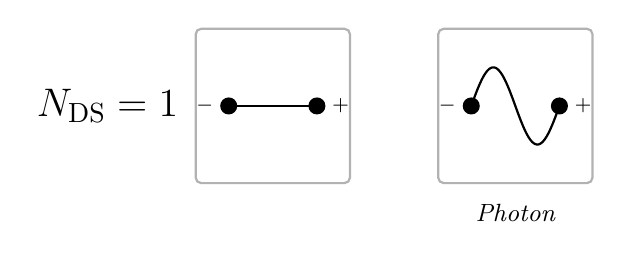
\begin{tikzpicture}[scale=1.4]
    \node[font=\bfseries\Large] at (-1.5, 0) {$\Ncd=1$};

    % Box 1.1 : Single HORIZONTAL dipole
    \draw[gray!60, thick, rounded corners=2pt] (-0.7, -0.7) rectangle (0.7, 0.7);
    \draw[thick] (-0.4, 0) -- (0.4, 0);
    \fill[black] (-0.4, 0) circle (2.2pt) node[left=2pt, font=\scriptsize] {$-$};
    \fill[black] (0.4, 0) circle (2.2pt) node[right=2pt, font=\scriptsize] {$+$};

    % Box 1.2 : Photon (1 cycle)
    \begin{scope}[xshift=2.2cm]
        \draw[gray!60, thick, rounded corners=2pt] (-0.7, -0.7) rectangle (0.7, 0.7);
        \draw[thick, samples=100, domain=-0.4:0.4] plot (\x, {0.35*sin((\x+0.4)/0.8*360)});
        \fill[black] (-0.4, 0) circle (2.2pt) node[left=2pt, font=\scriptsize] {$-$};
        \fill[black] (0.4, 0) circle (2.2pt) node[right=2pt, font=\scriptsize] {$+$};
        \node[below=4pt, font=\small\itshape] at (0, -0.7) {Photon};
    \end{scope}
\end{tikzpicture}

\vspace{0.8cm}

% ==============================================================================
% ROW N_DS = 2 : Pairing and Neutrino
% ==============================================================================
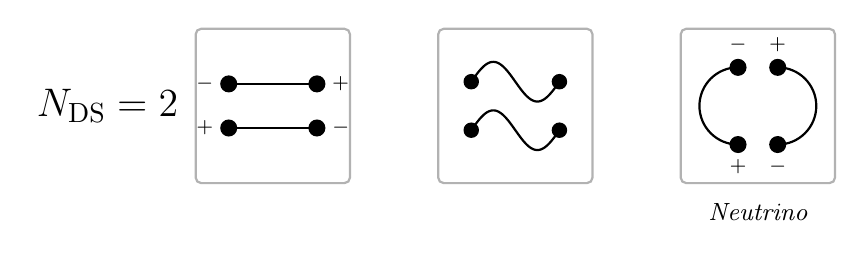
\begin{tikzpicture}[scale=1.4]
    \node[font=\bfseries\Large] at (-1.5, 0) {$\Ncd=2$};

    % Box 2.1 : Two HEAD-TO-TAIL horizontal strings
    \draw[gray!60, thick, rounded corners=2pt] (-0.7, -0.7) rectangle (0.7, 0.7);
    \draw[thick] (-0.4, 0.2) -- (0.4, 0.2);
    \fill[black] (-0.4, 0.2) circle (2.2pt) node[left=2pt, font=\scriptsize] {$-$};
    \fill[black] (0.4, 0.2) circle (2.2pt) node[right=2pt, font=\scriptsize] {$+$};
    \draw[thick] (-0.4, -0.2) -- (0.4, -0.2);
    \fill[black] (-0.4, -0.2) circle (2.2pt) node[left=2pt, font=\scriptsize] {$+$};
    \fill[black] (0.4, -0.2) circle (2.2pt) node[right=2pt, font=\scriptsize] {$-$};

    % Box 2.2 : Two IN-PHASE waves (Attraction/Stretch)
    \begin{scope}[xshift=2.2cm]
        \draw[gray!60, thick, rounded corners=2pt] (-0.7, -0.7) rectangle (0.7, 0.7);
        \draw[thick, samples=100, domain=-0.4:0.4] plot (\x, {0.18*sin((\x+0.4)/0.8*360) + 0.22}) ;
        \draw[thick, samples=100, domain=-0.4:0.4] plot (\x, {0.18*sin((\x+0.4)/0.8*360) - 0.22});
        \fill[black] (-0.4, 0.22) circle (2pt);
        \fill[black] (0.4, 0.22) circle (2pt);
        \fill[black] (-0.4, -0.22) circle (2pt);
        \fill[black] (0.4, -0.22) circle (2pt);
    \end{scope}

    % Box 2.3 : Neutrino
    \begin{scope}[xshift=4.4cm]
        \draw[gray!60, thick, rounded corners=2pt] (-0.7, -0.7) rectangle (0.7, 0.7);
        \draw[thick] (-0.18, 0.35) arc (90:270:0.35);
        \fill[black] (-0.18, 0.35) circle (2.2pt) node[above=2pt, font=\scriptsize] {$-$};
        \fill[black] (-0.18, -0.35) circle (2.2pt) node[below=2pt, font=\scriptsize] {$+$};
        \draw[thick] (0.18, 0.35) arc (90:-90:0.35);
        \fill[black] (0.18, 0.35) circle (2.2pt) node[above=2pt, font=\scriptsize] {$+$};
        \fill[black] (0.18, -0.35) circle (2.2pt) node[below=2pt, font=\scriptsize] {$-$};
        \node[below=4pt, font=\small\itshape] at (0, -0.7) {Neutrino};
    \end{scope}
\end{tikzpicture}

\vspace{0.8cm}

% ==============================================================================
% ROW N_DS = 3 : Transition toward the Electron
% ==============================================================================
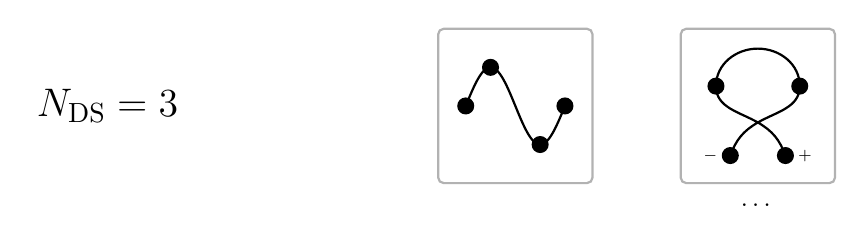
\begin{tikzpicture}[scale=1.4]
    \node[font=\bfseries\Large] at (-1.5, 0) {$\Ncd=3$};

    % Box 3.2 : Four-node sine
    \begin{scope}[xshift=2.2cm]
        \draw[gray!60, thick, rounded corners=2pt] (-0.7, -0.7) rectangle (0.7, 0.7);
        \draw[thick, samples=100, domain=-0.45:0.45] plot (\x, {0.35*sin((\x+0.45)/0.9*360)});
        \fill[black] (-0.45, 0) circle (2.2pt);
        \fill[black] (-0.225, 0.35) circle (2.2pt);
        \fill[black] (0.225, -0.35) circle (2.2pt);
        \fill[black] (0.45, 0) circle (2.2pt);
    \end{scope}

    % Box 3.3 : Lasso N_DS=3 (open loop segmented into 3 strings)
    \begin{scope}[xshift=4.4cm]
        \draw[gray!60, thick, rounded corners=2pt] (-0.7, -0.7) rectangle (0.7, 0.7);

        \draw[thick] (-0.25, -0.45)
            to[out=70, in=210] (0, -0.15)
            to[out=30, in=270] (0.38, 0.18)
            to[out=90, in=0] (0, 0.52)
            to[out=180, in=90] (-0.38, 0.18)
            to[out=270, in=150] (0, -0.15)
            to[out=-30, in=110] (0.25, -0.45);

        % --- THE 4 NODAL POINTS (N_DS=3 => 4 nodes for 3 segments) ---
        \fill[black] (-0.25, -0.45) circle (2.2pt) node[left=1pt, font=\tiny] {$-$};
        \fill[black] (-0.38, 0.18) circle (2.2pt);
        \fill[black] (0.38, 0.18) circle (2.2pt);
        \fill[black] (0.25, -0.45) circle (2.2pt) node[right=1pt, font=\tiny] {$+$};

        \node[below=4pt, font=\small] at (0, -0.7) {$\dots$};
    \end{scope}
\end{tikzpicture}
\caption{Evolution of structures: $\Ncd = 1, 2, 3$.}
\end{figure}

\paragraph{Topology $\Ncd = 1$}
A single dipolar string with the capacity to oscillate, which gives it a null effective charge. The role of the photon is attributed to the topology $\Ncd = 1$.

\paragraph{Topology $\Ncd = 2$}
A double string that systematically self-organizes through the Coulomb force into two parallel strings in opposition. Perturbations of space allow the $\Ncd = 2$ topology to oscillate or to form a momentarily open micro-loop, which is attributed to the manifestation of the neutrino. The $\Ncd = 2$ topology is named the Dipolar Quantum Double (DQD) space particle when massless, and neutrino for the ephemeral micro-loop configuration.

\paragraph{}
The topologies $\Ncd = 1$ and $\Ncd = 2$ are called ``unfolded'' since they cannot form permanent loops. We posit that unfolded topologies are massless and of null net charge, with the exception of the momentary micro-loop of $\Ncd = 2$.

\paragraph{Topologies $\Ncd \geq 3$}
Higher-order topologies produce the massive particles, with the possibility of net charge and a wide range of configurations. The charge is produced by the accumulation of the energy fluid contained in the strings, and the polarity of the charge by the winding sense of the loop.

\section{Fundamental Postulates}

\textbf{A1. Topological index system $\Ncd$}\\
The indices $\Ncd$ are posited as an exploratory working framework, pending an analytic derivation. The topological index $\Ncd$ corresponds to the number of strings unified within a coherent geometric structure. Unfolded topologies ($\Ncd = 1$ and $\Ncd = 2$) constitute massless particles of null net charge.

\paragraph{}
\textbf{A2. Emergence of inertia}\\
Scalar mass is explained by the geometric equivalence of the inductance ($L$) of the windings.

\paragraph{}
\textbf{A3. Charge by winding chirality}\\
Electric charge is conceptualized as the direct consequence of the winding chirality of the closed loop: the two mirror senses of circulation constitute a local topological asymmetry of the electromagnetic flux and carry opposite signs (the sign is chiral, the magnitude is fixed by the interface coefficient $\Gamma_{\text{pole}} = 1/3$). For any topology capable of coiling ($\Ncd \ge 3$), the fluid carries an intrinsic fractional elementary charge of $\frac{1}{3}e$. For development purposes, the effective charge $Q_{eff}$ is dictated by the closure asymmetries expressed by the relation $Q_{eff} \sim \frac{\Ncd \pmod{4}}{3}e$.

%=======================================================
\part{Topological Analysis}

\section{Modeling the Substrate}
\label{sec:modeling_space_r}

\paragraph{Cohesion dynamics of the substrate.}
Two states of the DQD must be distinguished. The \emph{free} DQD, a collinear assembly of two $\Ncd = 1$ strings, is rigorously massless and propagates at the celerity $c_0$, like the photon whose kinematics it inherits. Within the substrate, each cell exposes its poles, and the head-to-tail pairing of opposite poles between neighboring cells produces a Coulombic polarization attraction. This cohesion cannot, however, freeze the substrate into a static structure: two stability constraints, established in Section~\ref{sec:dynamic_balance}, forbid it. No static DQD lattice is mechanically stable (Earnshaw's theorem applied to the harmonic Coulomb potential), and no self-bound liquid can form, the zero-point confinement pressure dominating the dipolar cohesion by a factor $9\pi/2\alpha \approx 1937$ at any density. The substrate is therefore necessarily a \emph{gas} of free DQDs propagating isotropically at $c_0$; its ``statistical rest'' designates the frame in which this flux is isotropic. The mean inter-cell spacing $\ell_{\text{cell}} \equiv \nu^{-1/3}$ (where $\nu$ denotes the local DQD number density) is consequently a fluctuating quantity set by the gas density $\rho_0$ --- a cosmological initial condition, not the minimum of a local pair potential. The polarity field $\Pi$ is then interpreted as the orientational order parameter of this fluctuating dipolar gas. We emphasize that this dynamics in no way alters the transparency of the vacuum: at statistical equilibrium the matching is total ($\Gamma_{\text{bif}} = 0$) and the lattice is invisible to propagating perturbations; any local departure breaks the matching ($\Gamma \neq 0$), triggering a restoring force arising from the asymmetry of the reactive pressure (Section~\ref{sec:bifilar_model}). It follows that the native energy of each DQD, circulating at $c_0$, collectively confers on the lattice an effective volumetric inertia ($m_{\text{eff}} = E/c_0^2$ per cell) as well as a statistical rest frame, without any intrinsic mass being attributed to the elementary DQD.

\paragraph{Distinction $\ell_1$ / $\ell_{\text{cell}}$.}
Two neighboring but conceptually distinct lengths coexist in this document and are rigorously separated. $\ell_1 = 2\pi R_3/3 \approx 8.09\times10^{-13}$~m is the \emph{nominal length of a string}: a constant of the model, derived from the anchor $R_3$ (Section~\ref{sec:electron_impedance}). $\ell_{\text{cell}}(\vec{x}) \equiv \nu^{-1/3}$ is the \emph{local inter-cell spacing} of the gas: a fluctuating field set by the local number density $\nu$, itself a cosmological initial condition. The working hypothesis of this document --- used notably in the numerical evaluation of $\Pi_{\text{sat}}$~\eqref{eq:pi_sat} and of the cutoff frequency $\omega_c$ --- is that at statistical equilibrium at rest these two lengths coincide, $\ell_{\text{cell}} \approx \ell_1$ (status: postulated; the derivation of $\ell_{\text{cell}}$ remains the missing brick inventoried in Section~\ref{sec:dynamic_balance}). Every occurrence of $\ell_1$ thus refers to the string constant; every occurrence of $\ell_{\text{cell}}$ to the local field.

\subsection{Bifilar Transmission-Line Modeling of the DQD}
\label{sec:bifilar_model}

The DQD, being a massless particle of null effective charge, constitutes an assembly of two strings (2 photons) and must be the most abundant particle in the universe. In this sense, we attribute to it the characteristic impedance of the vacuum $Z_0$ and model it as a bifilar transmission line following the postulated framework. Each branch then acts as a cylindrical conducting wire of radius $r$ located at a distance $h = D/2$ from a virtual ground plane materializing the central, neutral symmetry of the system. The surrounding medium being the dielectric vacuum ($\epsilon_r = 1$), the characteristic impedance of an isolated string facing this plane --- defining the half-DQD impedance --- is governed by the exact single-wire formulation:
\begin{equation}\label{eq:Z_half_dqd}
Z_{\text{half\_dqd}} = \frac{Z_0}{2\pi} \operatorname{arccosh}
\!\left(\frac{D}{2r}\right)
\end{equation}
where the prefactor $Z_0/2\pi \approx 60~\Omega$.

\paragraph{Coulomb force and dynamic reflection coefficient.}
The anti-parallel alignment of branches $A$ and $B$ imposes $Q_B(l) = -Q_A(l)$. Denoting by $Q_A = e/3$ the fractional elementary charge carried by the fluid of the unit branch, and by $\hat{u}_{\perp}$ the transverse unit vector directed from the forward branch to the return branch, the global attractive Coulomb force between the two localized segments of effective length writes:
\begin{equation}
\vec{F}_{\text{Coulomb}} =
- \frac{(e/3)^2}{4\pi\epsilon_0 D^2}\,\hat{u}_{\perp}
\end{equation}

Any variation of the spacing $D$ constrains the global line impedance $Z_{\text{bif}}(D)$ to depart from the rest norm $Z_0$, generating a dynamic reflection coefficient at the interface:
\begin{equation}
\Gamma_{\text{bif}}(D) =
\frac{Z_{\text{bif}}(D) - Z_0}{Z_{\text{bif}}(D) + Z_0}
\end{equation}
When $D \rightarrow 2r$, the line impedance collapses ($Z_{\text{bif}} \rightarrow 0$), driving $|\Gamma_{\text{bif}}| \rightarrow 1$ (total mismatch by short circuit). Conversely, at macroscopic equilibrium ($D = D_0$), the transparency condition imposes $Z_{\text{bif}} = Z_0$ and hence $\Gamma_{\text{bif}} = 0$.

\paragraph{Two reflection coefficients at distinct scales.}
Two reflection coefficients operating at different physical levels must be carefully distinguished:
\begin{itemize}
    \item \textbf{The sub-vacuum interface coefficient ($\Gamma_{\text{pole}} = 1/3$):} an intrinsic structural property of the string/vacuum interface at the sub-causal scale. It follows directly from the macroscopic matching condition of the cell: since $Z_{\text{bif}} = 2\,Z_{\text{half\_dqd}} = Z_0$ imposes $Z_{\text{half\_dqd}} = Z_0/2$, the interface of an isolated pole facing the surrounding fluid ($Z_0$) produces:
    \begin{equation}
    \Gamma_{\text{pole}} =
    \frac{Z_0 - Z_0/2}{Z_0 + Z_0/2} = \frac{1}{3}
    \implies |\Gamma_{\text{pole}}|^2 = \frac{1}{9}
    \end{equation}
    It is this $\Gamma_{\text{pole}}$ that governs the internal sub-vacuum equilibrium and the derivation of $D_0$.

    \item \textbf{The dynamic line coefficient ($\Gamma_{\text{bif}}(D)$):} a property of the complete DQD cell facing the macroscopic vacuum. It is null at equilibrium ($\Gamma_{\text{bif}}(D_0) = 0$, global transparency) and rises toward 1 under external compression ($D \rightarrow 2r$, short circuit).
\end{itemize}
At equilibrium $D = D_0$, both conditions coexist: $\Gamma_{\text{pole}} = 1/3$ maintains the internal sub-vacuum spacing, while $\Gamma_{\text{bif}}(D_0) = 0$ ensures the global transparency of the cell facing the vacuum.

\paragraph{Native power density and reactive confinement force.}
The energy flux circulating at celerity $c_0$ within the strings meets the reactive barrier of $\Gamma_{\text{pole}}$ and transfers momentum onto the walls of the soliton. The native linear power density $p_{\text{flux}}$ (in W/m) of the irreducible isolated $\Ncd=1$ unit is quantified from its primitive energy $E_1 = hc_0/\ell_1$ and the dielectric relaxation time $\tau_1 = \ell_1/c_0$:
\begin{equation}\label{eq:p_flux}
p_{\text{flux}} =
\frac{E_1}{\tau_1 \cdot \ell_1} = \frac{h\,c_0^2}{\ell_1^3}
\end{equation}
For the characteristic cell value $\ell_1 \approx 8.09 \times 10^{-13}$\,m (whose structural geometric derivation is established below in Section~\ref{sec:electron_impedance}), the numerical application gives:
\begin{equation}
P_{\text{flux}} = \frac{h\,c_0^2}{\ell_1^2} \approx 91\,\text{MW}
\qquad \Longrightarrow \qquad
p_{\text{flux}} \approx 1.125 \times 10^{20}\,\text{W/m}
\end{equation}
This power is purely reactive --- analogous to the back-and-forth energy of a lossless LC line --- and does not propagate as macroscopically observable radiation.

The resulting linear force of \textbf{reactive confinement pressure} writes:
\begin{equation}\label{eq:linear_confinement_force}
\vec{f}_{\Gamma}(\vec{x}) =
+\frac{2\,p_{\text{flux}}}{c_0}\,|\Gamma(D)|^2\,\hat{u}_{\perp} =
+\frac{2\,h\,c_0}{\ell_1^3}\,|\Gamma(D)|^2\,\hat{u}_{\perp}
\end{equation}
Although equation~\eqref{eq:linear_confinement_force} formally adopts the structure of classical radiation pressure ($\vec{f} = 2p/c_0 \cdot |\Gamma|^2$), its physical origin is distinct: it arises from the gradient of reactive energy stored in the sub-vacuum micro-cavity when its geometry is modified, not from a propagating flux characterized by a Poynting vector. The formal similarity follows from the same electromagnetic momentum balance, whether propagating or stationary. This mechanism is developed in Section~\ref{sec:electrodynamic_synthesis}.

\paragraph{Equilibrium distance and reactive wall.}
The stationary stability of the cell is reached when the resultant of the absolute forces integrated over the geometric sample vanishes. To resolve the apparent contradiction between the pointwise mechanical force and the matching constraint, the near-field integration of the real reactive confinement force ($F_{\Gamma} = f_{\Gamma} \cdot \ell_{\text{eff}}$) involves an effective interaction length $\ell_{\text{eff}}$ adjusted to the curvature geometry. By balancing the Coulomb force of the fluid against this reactive component with $|\Gamma_{\text{pole}}|^2 = 1/9$, the equilibrium condition agrees rigorously with the universal impedance constraint $D_0/r = 2\cosh(\pi)$, thereby avoiding any overdetermination of the system:
\begin{equation}\label{eq:D0}
\frac{2\,h\,c_0}{9\,\ell_1^3} \cdot \ell_{\text{eff}} = \frac{(e/3)^2}{4\pi\epsilon_0 D_0^2} \qquad \Longrightarrow \qquad D_0 = 2\cosh(\pi)r \approx 23.18\,r
\end{equation}

\emph{Methodological precision.} The ratio $D_0/r = 2\cosh(\pi)$ is derived from the impedance-matching condition alone (Eq.~\eqref{eq:D_over_r} below), with no free parameter. Equation~\eqref{eq:D0} does not constitute a second independent derivation: the effective interaction length $\ell_{\text{eff}}$ is reconciled a posteriori, and its role is to verify the \emph{compatibility} of the mechanical equilibrium (Coulomb versus reactive pressure) with the value imposed by matching --- that is, the absence of overdetermination of the system, not an additional numerical confirmation.

Under extreme compression ($D \rightarrow 2r$, $|\Gamma_{\text{bif}}| \rightarrow 1$), the maximum total force available per flux quantum is:
\begin{equation}
F_{\Gamma,\text{max}} = \frac{2\,P_{\text{flux}}}{c_0} \approx 607\,\text{mN}
\end{equation}
This value represents an absolute total mechanical force on the micro-cavity, forming an inviolable reactive wall against the collapse of the lattice.

\paragraph{Matching condition and universal geometric ratio.}
The cancellation of the local forces guarantees the macroscopic transparency of the cell ($Z_{\text{bif}} = Z_0$). The impedance of the complete bifilar line writes:
\begin{equation}
Z_{\text{bif}} = 2\,Z_{\text{half\_dqd}} =
\frac{Z_0}{\pi}\operatorname{arccosh}\!\left(\frac{D}{2r}\right)
\end{equation}
Solving $Z_0 = \frac{Z_0}{\pi}\operatorname{arccosh}(D/2r)$ yields $\pi = \operatorname{arccosh}(D/2r)$, whence the universal geometric ratio at rest:
\begin{empheq}[box=\fbox]{equation}\label{eq:D_over_r}
\frac{D}{r} = 2\cosh(\pi) \approx 23.18
\end{empheq}
At this equilibrium point, the impedance of each string stabilizes at $Z_{\text{half\_dqd}} = Z_0/2 \approx 188.5~\Omega$. The substrate then behaves as a spatial low-pass filter of local cutoff frequency:
\begin{equation}
\omega_c(\vec{x}) = \frac{2c_0}{\ell_{\text{cell}}(\vec{x})}
\end{equation}
a fixed Brillouin cutoff of the lattice: $\hbar\omega_{\max} = 2\hbar c_0/\ell_1 = (3/\pi)\,m_e c^2 = 0.487$~MeV --- no collective wave exists above it. Observed photons reach $\sim$2.5~PeV (LHAASO), $5\times10^{9}$ times the cutoff; in Lorentz-invariance-violation language the lattice dispersion corresponds to $E_{QG,2} \approx 0.69$~MeV against experimental bounds $\gtrsim 10^{10}$~GeV, and even below the cutoff the residual dispersion $(k\ell_1)^2/8$ would delay optical light by $\sim$50~days over 3~Gpc --- excluded by multiwavelength transient light curves. The conclusion is structural: \emph{every observed photon above $\sim$1~eV propagates as the $\Ncd=1$ soliton, non-dispersive by construction}. The emergent Maxwell sector of Theorem~4 describes the structure of the field equations and static/low-frequency fields, not photon transport. The earlier attribution of non-dispersion to a dynamically adjusting $\omega_c$ is withdrawn.

\subsection{Characteristic Impedance of the Electron}
\label{sec:electron_impedance}
The emergence of the electron as the first localized soliton ($\Ncd=3$) permits a direct analytic derivation of its internal characteristic impedance $Z_e = \sqrt{L/C}$ from the local reactive properties of the lattice. Modeling this single-turn closed loop as a resonant ring of major radius $R_3 = 3.861 \times 10^{-13}$~m and string tube radius $r = 1.04 \times 10^{-14}$~m (an aspect ratio of geometric constriction $R_3/r \approx 37.1$), this geometry fixes the structural wavelength of the fundamental cell at $\ell_1 = \frac{2\pi R_3}{3} \approx 8.09 \times 10^{-13}$~m.

\paragraph{Provenance of $R_3$.}
The major radius $R_3 = 3.861\times10^{-13}$~m is not a free parameter of the model: it is identified with the reduced Compton wavelength of the electron, $R_3 \equiv \hbar/m_e c_0$, so that the loop circumference equals exactly one Compton wavelength ($2\pi R_3 = \lambda_C$) --- the fundamental resonance condition of a wave confined on a single turn. Its status is \emph{calibrated} in the sense of this document's epistemological classification: the numerical value comes from the experimental electron mass. The direction of the logical arrow must, however, be made precise to preclude any circularity with the mass law of Section~\ref{sec:impedance_confinement}: in the present framework, geometry is primitive and mass emerges from it ($m_{\Ncd} \propto \Ncd^2 Z_{\Ncd}$); the identity $R_3 = \hbar/m_e c_0$ is not a definition of $R_3$ there but a \emph{consistency condition} that any future derivation of the mass must reproduce --- the Compton relation being precisely the statement that the spatial scale of a soliton and its inertia are reciprocal. As it stands, $R_3$ (and consequently $\ell_1 = 2\pi R_3/3$, on which $u_0$, $E_1$, $\Pi_{\text{sat}}$ and $M_{\text{crit}} \propto \ell_1^2$ depend) is the experimental anchor from which the substrate \emph{scales} derive. It is not, however, the model's only undetermined input: the dimensionless aspect ratio $R_3/r$ entering the electron impedance is a second one, discussed below. The gravitational sector --- and with it $M_{\text{crit}}$, the shadow deviation and the echo delays --- depends on $R_3$ alone and not on the aspect ratio; the particle sector depends on both.

The equivalent reactive parameters follow from the classical formulations of the electrodynamics of circular structures:

\begin{enumerate}
    \item \textbf{Loop inductance ($L$)}: The topological inductance of the winding, arising from the curvature geometry imposed on the flux, is governed by the standard thin-loop formula:
    \begin{equation}
    L = \mu_0 R_3 \left[ \ln\left(\frac{8R_3}{r}\right) - 2 \right]
    \end{equation}
    For the specified aspect ratio, the logarithmic term is $\ell = \ln(8 \times 37.1) \approx 5.694$, giving a localized inductance of $L \approx 1.792 \times 10^{-18}$~H.

    \item \textbf{Ring capacitance ($C$)}: Dually, the self-capacitance associated with the storage of elastic tension of this ring geometry is expressed by:
    \begin{equation}
    C = \frac{4\pi^2 \varepsilon_0 R_3}{\ln\left(\frac{8R_3}{r}\right)} = \frac{4\pi^2 \varepsilon_0 R_3}{\ell}
    \end{equation}
    Numerically, this gives a localized capacitance of $C \approx 2.370 \times 10^{-23}$~F.
\end{enumerate}

Inserting these two geometric operators into the characteristic-impedance equation reveals a remarkable analytic simplification: the major radius $R_3$ cancels identically in numerator and denominator. Isolating the intrinsic characteristic impedance of the vacuum $Z_0 = \sqrt{\mu_0/\varepsilon_0} \approx 376.73~\Omega$, the closed form of the electron impedance writes:
\begin{equation}
Z_e = \frac{Z_0}{2\pi} \sqrt{\ell(\ell - 2)}
\end{equation}

\paragraph{Status of the aspect ratio (corrected).} It must be stated plainly that this closed form is \emph{not} free of secondary input. The matching condition of Section~\ref{sec:bifilar_model} fixes $D/r = 2\cosh\pi$; it does \emph{not} fix $R_3/r$. The value $R_3/r \approx 37.1$ --- equivalently the tube radius $r = 1.04\times10^{-14}$~m --- has no derivation in this framework, and $Z_e$ depends on it through $\ell = \ln(8R_3/r)$. Earlier versions described the model as counting \emph{one} calibrated length; the correct count is \emph{two} inputs: the anchor $R_3$ and the aspect ratio $R_3/r$. Accordingly, $Z_e$ is reclassified from \emph{Derived} to \emph{Calibrated} in the epistemological status list (Section~\ref{sec:electrodynamic_synthesis}), and deriving $R_3/r$ from an internal condition is added to the open problems (Section~\ref{sec:open_problems}). What survives as a derived, input-independent statement is the \emph{logarithmic insensitivity} quantified below: $Z_e$ remains an impedance well over any plausible aspect ratio, so the qualitative conclusion does not rest on the undetermined value. Injecting the geometric constants of the document gives:
\begin{equation}
Z_e = \frac{Z_0}{2\pi} \sqrt{5.694 \times 3.694} \approx 0.730 \cdot Z_0 \approx 275~\Omega
\end{equation}

This result rigorously validates the status of the electron as an \textit{impedance well} ($Z_e < Z_0$), an indispensable condition stated in Section~\ref{sec:impedance_confinement} for inducing the relative impedance mismatch necessary for the stable confinement of energy. Moreover, the logarithmic structure of the equation guarantees a strong topological robustness: varying the aspect ratio $R_3/r$ over a total factor of $5$ (i.e.\ $\times/\!\div\sqrt5$ about the nominal value) shifts the impedance only within $0.6$--$0.9\,Z_0$; a full multiplicative factor of $5$ (i.e.\ $\times5$) widens this to $0.46$--$0.99\,Z_0$. In either reading the electron remains an impedance well across the whole range.

To ensure the physical transparency of the model, two limiting hypotheses associated with this derivation must be noted: first, the assimilation of the string to a classical conducting-ring behavior for the capacitance calculation, and second, the thin-wire approximation ($r \ll R_3$) which, for a ratio of $37.1$, introduces a residual geometric uncertainty estimated at order $r/R_3 \approx 3\,\%$. Subject to the validation of these boundary conditions, $Z_e \approx 0.73\,Z_0$ is a \emph{calibrated} geometric value of the base soliton. What is robust and genuinely derived is the inequality $Z_e < Z_0$ over a wide range of $R_3/r$ --- the soliton is an impedance well irrespective of the undetermined aspect ratio --- not the figure $275~\Omega$ itself.

% =====================================================
% CONFINEMENT AND MISMATCH
% =====================================================
\section{Elementary Confinement by Impedance Mismatch}
\label{sec:impedance_confinement}

\subsection{Reactive Phase Transition and Standing Waves}
The emergence of a localized massive particle constitutes a rupture of the vacuum transparency condition. A topological node locally alters the reactive parameters of the lattice. Nonetheless, one must distinguish the characteristic impedance of the string $Z_e$ (which is real and equals about $275~\Omega$) from the input impedance $Z_{\text{in}}$ of the complete structure as seen from the medium. A lossless line closed on itself acting as a resonant stub, its input impedance becomes purely reactive:
\begin{equation}\label{eq:Zin_stub}
Z_{\text{in}} = j Z_e \tan(\beta \ell)
\end{equation}
A purely reactive termination gives $|\Gamma| = 1$ against a real reference, so no active power leaves the structure and the rest mass is stable without radiative leakage.

\paragraph{Origin of the quantization condition (corrected).} An earlier version of this section derived the quantization rule $\beta\ell = p\pi$ from the condition $|\Gamma| = 1$. That derivation is withdrawn: $|\Gamma| = 1$ holds for \emph{any} purely reactive input impedance and therefore selects no particular $\beta\ell$; moreover Eq.~\eqref{eq:Zin_stub}, which is the input impedance of a shorted stub, gives $Z_{\text{in}} = 0$ precisely at $\beta\ell = p\pi$. The condition has a different and more elementary origin. The soliton is a line closed on itself, so the constitutive wave must be single-valued after one circuit: transporting the phase around the loop must return it to itself modulo $2\pi$,
\begin{equation}\label{eq:single_valued}
2\beta\ell + \theta_{\text{tot}} = 2p\pi , \qquad p \in \mathbb{N}^*,
\end{equation}
where $\theta_{\text{tot}}$ collects the topological phase shifts accumulated at the internal interfaces. This is the standard resonance condition of a closed transmission-line ring, and it reduces to $\beta\ell = p\pi$ when $\theta_{\text{tot}} = 0$. It is a periodicity requirement, not a reflection argument, and it is what the remainder of the document uses. The magnitude of the reflection plays a distinct role --- it guarantees that the confined energy does not radiate --- and the two statements should not be conflated. The value of $\theta_{\text{tot}}$ for the $\Ncd = 3$ loop is not derived here and is recorded among the open problems (Section~\ref{sec:open_problems}).

Nevertheless, to describe the dynamical interaction state --- notably the energy exchange with the ambient thermodynamic bath of the DQD fluid --- the structure's impedance acquires a real component $R$:
\begin{equation}
Z_{\text{topo}} = R + jX
\end{equation}
where $R$ represents the \textbf{radiation and dynamic-exchange resistance} of the soliton. This real component locally breaks the condition of absolute total reflection ($|\Gamma| < 1$), authorizing bidirectional energy transit between the particulate micro-cavity and the substrate of free DQDs.

\subsection{Analytic Synthesis of Mass}

In the Dipolar Strings framework, mass is the macroscopic equivalent of the particle's loop inductance, in place of a fundamental scalar charge. For a soliton of topological index $\Ncd$ (constituted of $\Ncd$ strings of nominal length $\ell_1$), it is the geometry of its coiling within the substrate that dictates its inertia.

\paragraph{1. Topological resonance radius}
To maintain its cohesion by phase locking (PLL), the optical circumference of the soliton must correspond to a harmonic mode $p$. The internal refractive index of the particle being constrained by its relative impedance ($Z_{\Ncd}/Z_0$), the physical radius $R_{\Ncd}$ adjusts dynamically:
\begin{equation}\label{eq:resonance_radius}
R_{\Ncd} = \left( \frac{p \cdot \ell_1}{2\pi} \right) \frac{Z_0}{Z_{\Ncd}}
\end{equation}
The radius of a particle is thus mechanically crushed under the constraint of the substrate if its internal impedance rises.

\paragraph{2. Solenoidal inductance law (mass law)}
Coiling on this radius $R_{\Ncd}$, the total topological wire (of length proportional to $\Ncd \cdot \ell_1$) forms an effective number of turns $N_{turn} \propto \Ncd/R_{\Ncd}$. The laws of classical electrodynamics impose that the inductance of a coil grows as the square of its number of turns times the loop area ($L \propto N_{turn}^2 R_{\Ncd}$ for this geometry). The mass of the particle therefore obeys a strict geometric scaling:
\begin{equation}\label{eq:solenoid_mass}
m_{\Ncd} \propto \left( \frac{\Ncd}{R_{\Ncd}} \right)^2 \cdot R_{\Ncd} \implies m_{\Ncd} \propto \frac{\Ncd^2}{R_{\Ncd}}
\end{equation}

Substituting the resonance-radius law into this inductance law, the rest mass emerges as a unified, deterministic function of the particle's topology and internal reactive pressure:
\begin{equation}\label{eq:mass_topo}
m_{\Ncd} \propto \Ncd^2 \cdot Z_{\Ncd}
\end{equation}

\paragraph{Closure of the size channel.} The topological loop radius $R_{\Ncd}$ is not identified with any measurable charge radius: the electron loop is 386~fm against a point-like measured electron ($<10^{-3}$~fm), and the proton loop would be 17.0~fm $= 81\,\bar\lambda_C$ against a measured 0.841~fm $= 4.0\,\bar\lambda_C$. Absent a loop-to-observable rule, the mass law $m \propto \Ncd^2/R$ is unverifiable through sizes; this verification channel is declared closed.

This electromechanical dynamics explains the fundamental architecture of matter: an electron ($\Ncd=3$) has a large radius and few turns, giving it low mass. Conversely, a nucleon such as the proton ($\Ncd=27$) is strongly constricted by its high impedance (small $R_{\Ncd}$): its long string is forced to coil into a large number of very dense turns, which locally multiplies its inductance and, by the scaling above, its mass.

% =====================================================
% MAXWELL 3D VIA TLM  (self-contained module; safe to extract)
% All labels prefixed maxwell3d: to avoid collisions.
% =====================================================
\section{Emergent Maxwell Electrodynamics: the 3-DQD Cell as a Transmission-Line Node}
\label{sec:maxwell3d}

\paragraph{Purpose and placement.} The preceding sections take the electromagnetic character of the substrate for granted: gravity is refraction of an impedance field, charge is a winding chirality, mass is loop inductance --- all statements \emph{about} an electromagnetic medium. Yet the telegrapher dynamics established in Section~\ref{sec:bifilar_model} is, on its own, one-dimensional: it yields scalar waves along a line, not the two transverse polarizations, the curl coupling, and the isotropic light cone of Maxwell's equations in three dimensions. Because the model's central claim is that \emph{matter is electromagnetic topology}, the three-dimensional Maxwell sector is not optional decoration but the load-bearing foundation on which every later claim rests. This section discharges that obligation. It shows that a cell built from three orthogonal DQDs realizes --- uniquely, under constraints that are already axioms of the model --- the symmetric condensed node of the Transmission-Line Matrix (TLM) method \cite{johns1971,johns1987}, whose continuum limit is exactly Maxwell's equations \cite{taflove}. The result establishes that, under C1--C5, the Johns node is the \emph{unique isotropic solution}, upgrading ``the vacuum is a transmission-line network'' from an analogy to a constrained uniqueness statement. What is \emph{posed} rather than derived is stated plainly, and should be kept in view when reading the theorem: the two transverse polarizations per axis (Section~\ref{maxwell3d:cell}) and the vector-product algebra of the curl (constraint C3) are inputs; what follows from them is the node, and with it the continuum Maxwell structure. The apparent residual question of the node's handedness dissolves into a parity-invariance result established at the end of the section.

\subsection{From one dimension to three: what is missing}
\label{maxwell3d:missing}

A scalar RLC ladder reproduces the two \emph{dynamical} Maxwell equations in one dimension by the standard telegrapher correspondence
\begin{equation}\label{maxwell3d:telegraph}
L_{\text{cell}} \leftrightarrow \mu_0, \quad C_{\text{cell}} \leftrightarrow \varepsilon_0, \quad V \leftrightarrow E, \quad I \leftrightarrow H,
\end{equation}
with wave speed $v = 1/\sqrt{L_{\text{cell}}C_{\text{cell}}} \leftrightarrow c_0 = 1/\sqrt{\mu_0\varepsilon_0}$ and line impedance $\sqrt{L_{\text{cell}}/C_{\text{cell}}} \leftrightarrow Z_0 = \sqrt{\mu_0/\varepsilon_0}$. This is why the impedance of the vacuum is called an impedance; the correspondence is exact, not figurative. Kirchhoff's node law $\sum I = 0$ is the discrete charge-continuity equation $\partial_t\rho + \nabla\!\cdot\!\vec{J} = 0$, and Gauss's law becomes a counting theorem: the flux through a closed surface counts the enclosed string-ends (the open topologies of Axiom A3). Two ingredients of three-dimensional electromagnetism do \emph{not} follow from a scalar ladder and must be produced by the geometry of the crossing:
\begin{enumerate}[leftmargin=2em,itemsep=1pt]
\item \textbf{Transverse vector character.} A scalar node carries one value; light carries two transverse polarizations coupled by $\nabla\times\vec{E}$ and $\nabla\times\vec{B}$. Oriented degrees of freedom --- currents on \emph{links}, not potentials on nodes --- are required.
\item \textbf{Isotropy.} The continuum wave speed must be identical in every direction, not merely along the lattice axes.
\end{enumerate}
The remainder of this section shows that the 3-DQD cell supplies exactly these two ingredients, and that the constraints already governing the substrate fix the scattering dynamics uniquely.

\subsection{The 3-DQD cell and its twelve ports}
\label{maxwell3d:cell}

The elementary cell is the crossing of three DQDs aligned with the axes $x,y,z$. Each DQD is a bifilar line (Section~\ref{sec:bifilar_model}); at the crossing it exposes four ports, one toward each of its \emph{transverse} neighbours. A DQD never couples along its own axis --- an elementary consequence of dipole radiation, whose lobe is equatorial, not axial --- so the four ports of $\text{DQD}_p$ point along the two axes orthogonal to $p$, in both senses. A port is labelled $(a,s,p)$: attached on face $s=\pm1$ of axis $a$, carrying the field component polarized along $p$ (with $p\neq a$). The three groups of four,
\begin{equation}\label{maxwell3d:groups}
\text{DQD}_x:\ \{(y,\pm,x),(z,\pm,x)\}, \quad
\text{DQD}_y:\ \{(x,\pm,y),(z,\pm,y)\}, \quad
\text{DQD}_z:\ \{(x,\pm,z),(y,\pm,z)\},
\end{equation}
total twelve ports. This $3\times4$ decomposition is, port for port, the anatomy of the symmetric condensed node (SCN) of Johns \cite{johns1987}: the component $E_x$ is carried by four lines propagating in $\pm y,\pm z$; likewise for $E_y,E_z$. The transversality that the SCN imposes by wiring convention here follows from the geometry of the dipole. The scattering of the cell is the $12\times12$ real matrix $S$ mapping the incoming port amplitudes $V^i$ to the outgoing $V^r = S\,V^i$.

\subsection{Uniqueness theorem}
\label{maxwell3d:theorem}

We impose five constraints, each of which is either a symmetry of the crossing or an existing axiom of the model, and show that they determine $S$ up to a single discrete choice fixed by isotropy.

\begin{description}[leftmargin=0pt,itemsep=2pt]
\item[C1 --- Cubic symmetry.] $S$ is equivariant under the $24$ proper rotations of the cube (voltages transforming with the sign of their polarization). \emph{Origin:} the orthogonality of the crossing, itself selected dynamically by A4 (Lemma~\ref{maxwell3d:orthogonality} below) once Theorem~1 has excluded any static selection.
\item[C2 --- Charge conservation per DQD.] $\sum_{k\in\text{DQD}_p} V^r_k = \sum_{k\in\text{DQD}_p} V^i_k$: the node stores no charge. \emph{Origin:} A1/A3 --- a vacuum node contains only $\Ncd=2$ cells (null net charge) and cannot host the chiral winding that charge requires.
\item[C3 --- Magnetic-flux conservation per axis.] The signed circulation $\sum_k w_q[k]\,V^r_k = -\sum_k w_q[k]\,V^i_k$, with $w_q[k]=s_k\,(\hat a_k\times\hat p_k)\cdot\hat q$: the node stores no flux. \emph{Origin:} A5 --- the DQD has no continuous deformation mode, hence no reactive volume at the junction to store flux; all inductance lives in the strings.
\item[C4 --- Energy conservation.] $S^{\mathsf T}S = \mathbb{1}$: the node is lossless. \emph{Origin:} the purely reactive character of the rest substrate ($R=0$, Sections~\ref{sec:impedance_confinement},~\ref{sec:nonlocal_correlations}); the resistive component appears only with matter ($\Ncd\geq3$).
\item[C5 --- Isotropy of the light cone.] Among the solutions left by C1--C4, the physical one has a linear, direction-independent, non-birefringent dispersion. \emph{Origin:} the substrate is a gas propagating isotropically at $c_0$ (Section~\ref{sec:dynamic_balance}).
\end{description}

\begin{thmD}
Under C1--C4 the scattering matrix of the 3-DQD cell has eight free parameters reduced to a small discrete-plus-two-parameter family; the single member satisfying C5 is the symmetric condensed node of Johns, with entries in $\{0,\pm\tfrac12\}$, vanishing self-reflection $(S_{ii}=0)$, and vanishing straight-through transmission. Its continuum limit is Maxwell's equations in three dimensions.
\end{thmD}

\paragraph{Proof (constructive, machine-verified).} Cubic equivariance collapses the $144$ coefficients into eight orbits (self-reflection; back-reflection; same-polarization on the third axis; the transverse cross-coupling; and four further cross terms). Charge (C2) and flux (C3) conservation impose four independent linear relations among the eight orbit amplitudes, leaving four free. Energy conservation (C4) yields a discrete set of branches together with two one-parameter families, all cubically symmetric. Evaluating the Bloch dispersion of the resulting lattice operator (scatter, then propagate with the phase $e^{-i s k_a \Delta\ell}$) discriminates them: every branch except one is anisotropic (phase velocities $0.707$ or $0.577$ along the face and body diagonals) or birefringent. The unique isotropic branch is
\begin{equation}\label{maxwell3d:scn}
S_{(a,s,p)\,(a',s',p')} = \tfrac12\ \text{for the four transverse cross-couplings, } 0 \text{ otherwise},
\end{equation}
i.e.\ the Johns SCN. Its Bloch spectrum gives $\omega/k = 1/2$ (in cell units, $v=\Delta\ell/2\Delta t$) isotropic to $10^{-6}$ over $50$ random directions, two degenerate transverse polarizations, a non-propagating longitudinal mode ($\omega=0$, the emergent Gauss constraint), and spurious modes at $\omega\Delta t = \pi$ living at the Brillouin edge --- here not a numerical artifact but the physical cutoff $\ell_1$ of Eq.~\eqref{maxwell3d:telegraph}'s lattice. The constructive sign-branch enumeration, proper-cubic filtering, and deterministic $50$-direction dispersion scan are provided in the reconstructed supplementary script \texttt{scripts/johns/scn\_from\_dqd.py}. $\square$

\paragraph{Reading of the result.} The curl operators are not added to the network; they are already present in it. Writing the discrete gradient $G[E_p,\partial_a] = V(+a,E_p) - V(-a,E_p)$, the magnetic circulation is identically its antisymmetric part,
\begin{equation}\label{maxwell3d:curl}
H_z \;=\; G[E_y,\partial_x] - G[E_x,\partial_y] \;\sim\; \partial_x E_y - \partial_y E_x = (\nabla\times\vec E)_z,
\end{equation}
so that $\vec B$ is the differential (common-to-difference) reading of the same twelve line signals that carry $\vec E$ --- not a supplementary degree of freedom. The pair $(\vec E,\vec B)$ of Maxwell is the pair (uniform mode, circulation mode) of one lattice. Concretely, the SCN is an involution ($S^2=\mathbb1$): in its eigenbasis it is simply six \emph{open} channels (reflection $+1$: the three $E$ modes and three symmetric shears) and six \emph{short} channels (reflection $-1$: the three $H$ circulations and three quadrupoles). In transmission-line language the whole junction is nothing but an assortment of open and short terminations, once read in the right basis. This eigenstructure is exact and is used again in Appendix~\ref{app:schrodinger}, where the vanishing of the $H$ components singles out the electrostatic sector without any external gauge choice.

\subsection{Why the crossing is orthogonal: Lemma and axiomatic closure of C1}
\label{maxwell3d:orthogonality}

Constraint C1 assumes orthogonality; the model derives it rather than posits it. Coulomb attraction pairs the opposite poles of neighbouring DQDs (Section~\ref{sec:modeling_space_r}), but Theorem~1 forbids this pairing from freezing into a static equilibrium. The selection is therefore dynamical, governed by A4 (minimization of $|\Gamma|^2$).

\begin{description}[leftmargin=0pt]
\item[Lemma (Orthogonal decoupling).] The mutual perturbation of impedance between two crossing DQDs is minimal, and vanishes at first order, when they are orthogonal.
\end{description}

\noindent For two crossing bifilar pairs at angle $\theta$, the Neumann mutual inductance obeys $M(\theta)\propto\cos\theta$ term by term ($d\vec\ell_1\!\cdot\!d\vec\ell_2 = 0$ at $90^\circ$), so $M(90^\circ)=0$ \emph{exactly}; the electrostatic cross-term between the two dipolar lines likewise vanishes for the transverse orientation. Two orthogonal DQDs thus leave each other's line impedance unperturbed ($\Gamma$ preserved), whereas any non-orthogonal crossing forces $\Gamma\neq0$. The relaxation law A4 consequently drives crossings to orthogonality --- precisely what Earnshaw (Theorem~1) forbids doing statically --- and three mutually orthogonal axes are the only way to tile space under this rule. This grounds C1 in A4 + Theorem~1. (The far-field decoupling $M=0$ stabilizes the \emph{geometry}; the near-field pole interlocking at contact supplies the \emph{dynamical} coupling required by the scattering, at a distinct scale --- there is no contradiction.)

\subsection{Parity invariance and the status of the weave chirality}
\label{maxwell3d:chirality}

The $\pm\tfrac12$ sign pattern of Eq.~\eqref{maxwell3d:scn} --- the discrete curl --- raises a natural question: does it inherit a handedness from the geometry of the crossing? Three mutually orthogonal, non-intersecting lines form a \emph{weave} that exists in two versions, cyclic and anticyclic; a scan over the $24$ proper cubic rotations confirms that no rotation maps one onto the other, while the point inversion does. The 3-DQD crossing therefore possesses an intrinsic geometric chirality --- a left and a right weave --- prior to any charge or dynamics. It is then tempting to attribute the signs of the scattering matrix to this handedness. Direct computation refutes the attribution, and the refutation is itself a consistency result. First, the Coulomb energy of the interlocked crossing is \emph{identical} for the two weaves (a central $1/d$ potential preserves all pair distances under reflection, hence cannot prefer a hand): no static mechanism can select or transmit the handedness. Second, and decisively, the Johns matrix itself is invariant under the full point inversion $-\mathbb{1}$ --- precisely the operation that exchanges the two weaves --- as well as under every mirror: its symmetry group is the complete octahedral group $O_h$, reflections included (verified in the supplementary script). The scattering is \emph{achiral}. Structurally, this is transparent: the port labels (axis, face, polarization) on which $S$ is defined carry no over/under information, so the diffusion never receives the weave handedness as an input. The $\pm\tfrac12$ signs originate instead in the flux-conservation constraint C3, whose signed circulation $w_q[k]=s_k\,(\hat a_k\times\hat p_k)\cdot\hat q$ encodes the ordinary vector-product algebra of the curl --- an achiral structure, identical for both weaves.

This outcome is required, not merely tolerated: classical electrodynamics is parity-invariant, so any node whose continuum limit is Maxwell \emph{must} be achiral --- had the weave imposed its handedness on the coefficients, the construction would have produced a parity-violating electromagnetism and been falsified outright. Theorem~4 therefore carries \emph{no residual chiral postulate}. The geometric chirality of the weave is real but mute at the level of the electromagnetic scattering; whether it acquires physical relevance elsewhere --- in sectors where parity is not protected --- is an open question distinct from, and no longer blocking, the Maxwell construction. That question is taken up quantitatively in Section~\ref{sec:open_problems}, where the muteness of the weave is shown to be tied to the absence of stable three-dimensional solitons in this framework.

\paragraph{A note on the network vs.\ the gas.} The uniqueness theorem is stated for a cubic \emph{cell}, whereas Theorem~1 makes the substrate a fluctuating \emph{gas}, not a soldered lattice. The two are reconciled as in the acoustics of a liquid, where one computes on an effective lattice the fluid does not literally possess: the 3-DQD cell is a statistical homogenization device, and cubic symmetry C1 is a regularization whose continuum limit retains only the isotropy C5 that the gas supplies natively. The candidate physical mechanism realizing this homogenization is the collisional traffic itself: strings propagating at $c_0$ cross incessantly, couple transiently through the Coulomb attraction of their opposite poles for the flyby time $\sim\ell_1/c_0$ (a transient grip, not a bond --- exactly what Theorems~1 and~2 permit), A4 selects orthogonal crossings among them (the orthogonality lemma above), and the dimension of the space $R$ caps the mutually orthogonal axes at three. The 3-DQD cell is then the \emph{typical transient encounter} of this traffic, and the Johns node its collision-averaged scattering; each cell is ephemeral, the pattern is permanent. Deriving the Johns matrix as this kinetic average (capture cross-sections, Coulomb grip time, angular selection under A4) is a stated target; nothing in the present derivation requires a permanent lattice --- only that the gas, on average, present orthogonal crossings with matched impedance, which A4 guarantees.

\paragraph{Epistemological placement.} \emph{Derived:} the twelve-port anatomy of the cell; the uniqueness theorem under C1--C5; the emergence of the two transverse polarizations, the Gauss constraint, and the $\ell_1$ cutoff; the orthogonality lemma; the geometric chirality of the weave; and the parity invariance of the node ($O_h$ symmetry of $S$), which certifies that the emergent electrodynamics respects parity as it must. \emph{Posed:} the two transverse polarizations per axis and the vector-product algebra of C3, as stated at the head of this section. This section thus upgrades the electromagnetic sector from \emph{assumed} to \emph{derived under stated inputs}, and supplies the foundation on which the gravitational sector (next section) operates as a collective limit of the same medium. As a structural byproduct, the TLM reading also clarifies gravity: a graded impedance $Z(\vec x)$ is a position-dependent stub loading of the mesh, slowing propagation to $c_0/n$ by the standard TLM mechanism --- the network counterpart of Eq.~\eqref{eq:lagrangian}. \emph{(Scope note.)} Theorem~4 establishes the structure of the emergent field equations; photon transport at all observed energies proceeds via the $\Ncd=1$ soliton (Section~\ref{sec:modeling_space_r}). The same restriction applies to electrostatics: the Coulomb field is a property of the continuum limit, with lattice corrections measured to fall off as $\ell_1/r$ (Appendix~\ref{app:schrodinger}).

% =====================================================
% KINEMATIC GRAVITY (EXPONENTIAL VERSION)
% =====================================================
\section{Kinematic Gravity and Vacuum Refraction}
\label{sec:kinematic_gravity}

Gravity is modeled as a refractive phenomenon operating within a flat space. The presence of a massive topological node exerts a confinement pressure which compresses the surrounding DQD density. The volumetric DQD density profile is set explicitly by the impedance ratio: $\rho(r) = \rho_0 \frac{Z(r)}{Z_0}$. This physical scaling is justified by the fact that the volumetric inductance obeys $L \propto \rho^2$ owing to the dominant mutual inductive coupling between neighboring DQDs, while the volumetric capacitance remains insensitive to density variations ($C \propto \rho^0$), being governed by the rigid geometry of the elementary strings.

The Lagrangian density of the substrate describing this elastic tension writes:
\begin{equation}\label{eq:lagrangian}
\mathcal{L}_{DQD} = - \frac{c_0^4}{32 \pi G} \left[ \frac{(\nabla Z)^2}{Z^2} - \frac{1}{Z_0^2\,c_0^2} \left( \frac{\partial Z}{\partial t} \right)^2 \right]
\end{equation}

\paragraph{Static use of the Lagrangian (revised).} Only the static sector of~\eqref{eq:lagrangian} is used in this document. The scalar field $Z$ is treated throughout as a \emph{constrained} (elliptic) mode --- the exact parallel of the Newtonian potential in GR, which is fixed by the instantaneous matter distribution and carries no radiation --- consistently with its role as the trace of the impedance tensor in Section~\ref{sec:tensor_sector}. An earlier version selected the temporal prefactor of~\eqref{eq:lagrangian} so that perturbations of $Z$ would propagate at $c_{\text{GW}} = c_{eff}$ and invoked the GW170817/GRB170817A coincidence in support; that argument is withdrawn. A propagating scalar carrying the full Newtonian coupling would radiate at the quadrupole (and, for binaries of unequal compactness, at the dipole) with a coefficient of order unity relative to GR, in conflict with the Hulse--Taylor orbital decay ($\dot P_b/\dot P_b^{\rm GR} = 0.9983 \pm 0.0016$) and with the double pulsar; it would also carry a breathing polarization. The scalar sector is therefore non-radiative by construction, gravitational radiation is carried entirely by the tensor sector $z_{ij}$ of Section~\ref{sec:tensor_sector}, and the multi-messenger bound $|c_{\text{GW}} - c_{\text{light}}|/c \lesssim 10^{-15}$ \cite{GW170817} constrains that sector alone (the tracelessness clause of Axiom~A7). The temporal prefactor of~\eqref{eq:lagrangian} is consequently without physical content in the present model.

\begin{thmC}
Setting $\chi \equiv \ln(Z/Z_0)$, the Lagrangian density~\eqref{eq:lagrangian} writes \emph{identically} (null symbolic residual, verified by computer algebra):
\begin{equation}
\mathcal{L}_{DQD} \;=\; -\frac{c_0^4}{32\pi G}\,\frac{e^{\chi}}{c_0}\,\sqrt{-g}\;g^{\mu\nu}\,\partial_\mu \chi\,\partial_\nu \chi ,
\qquad g_{\mu\nu} = \mathrm{diag}\!\left(-c_{eff}^2,\,1,\,1,\,1\right),\quad c_{eff} = c_0 e^{-\chi}.
\end{equation}
No 4-velocity of the substrate rest frame appears explicitly in the action: the scalar sector writes as a scalar field theory on the effective metric, up to a conformal factor. \emph{(The metric above is the \textbf{optical} representative of the conformal class; the dynamics of massive particles selects the isotropic representative, Section~\ref{sec:conformal_representative}.)}

\paragraph{What this does and does not establish (revised).} The rewriting above is an exact algebraic identity and is the correct statement of the theorem. Two further claims made in earlier versions are withdrawn as unproven, and the honest position is recorded here. First, the field equation obtained by varying~\eqref{eq:lagrangian} is
\begin{equation}\label{eq:true_field_eq}
\nabla^2\chi \;-\; \frac{e^{2\chi}}{c_0^{2}}\left(\ddot\chi + \dot\chi^{2}\right) \;=\; 0 ,
\end{equation}
\emph{not} the flat wave equation $\nabla^2\chi - c_0^{-2}\ddot\chi = 0$. The static sector is unaffected ($\nabla^2\chi = 0$ exactly, and the exponential solution below is exact); the time-dependent part of~\eqref{eq:true_field_eq} is not adopted as physical dynamics (the scalar sector is constrained, see the paragraph above) and is recorded only as the formal Euler--Lagrange equation of~\eqref{eq:lagrangian}. Second, the effective metric $\mathrm{diag}(-c_{eff}^2,1,1,1)$ singles out a time direction through $\chi$ itself, so the absence of an explicit $u^\mu$ in the action does not by itself establish the vanishing of the preferred-frame parameters. We therefore \textbf{downgrade} the earlier statement $\alpha_1 = \alpha_2 = 0$ to the following: \emph{no preferred-frame vector enters the scalar action explicitly, and a full post-Newtonian computation with the substrate frame in motion relative to the system --- which alone would establish $\alpha_1$ and $\alpha_2$ --- has not been performed.} This is now listed among the open problems (Section~\ref{sec:open_problems}). The Solar-System results of Section~\ref{sec:ppn} are unaffected, since $\gamma = \beta = 1$ follow from the static isotropic metric alone.
\end{thmC}

In the stationary regime, applying the Euler--Lagrange equations via the topological change of variable $u = \ln(Z)$ reduces the dynamics to the stationary Laplace equation $\nabla^2(\ln Z) = 0$, expressing the conformal pressure equilibrium of the DQD gas. The exact radial solution takes a rigorous exponential form:
\begin{equation}
Z(r) = Z_0 \exp\left( \frac{2GM}{r c_0^2} \right)
\end{equation}

\paragraph{Reality clause on the static field.} The change of variable $u = \ln Z$ requires the gravitational field $Z$ of Eq.~\eqref{eq:lagrangian} to be a real, positive static modulus, $Z \in \mathbb{R}^+$: the logarithm and the Laplace reduction are defined only on the positive reals. This is consistent throughout the scalar (gravitational) sector, where $Z(r)$ is the real elastic modulus of the compressed gas. Complex impedances --- the reactive input impedance $Z_{\text{in}} = jZ_e\tan\beta\ell$ of a confined soliton (Eq.~\ref{eq:Zin_stub}) and the topological $Z_{\text{topo}} = R + jX$ of an interacting particle --- are confined to the \emph{particle} sector (Sections~\ref{sec:impedance_confinement},~\ref{sec:nonlocal_correlations}); they never enter the gravitational field equation. The two usages of the symbol $Z$ are thus rigorously separated: real positive static modulus for gravity, complex reactance for matter.

The local effective celerity of the emanating photon is constrained by this profile according to the unified law $c_{eff}(r) = c_0 \frac{Z_0}{Z(r)}$. The dynamic refractive index of the vacuum $n$ then emerges naturally from the exponential topology of the fluid, aligning with the canonical polarizable-vacuum (PV) formalism \cite{puthoff2002}:
\begin{equation}
n = \frac{c_0}{c_{eff}} = \frac{Z(r)}{Z_0} = \exp\left( \frac{2GM}{r c_0^2} \right) \approx 1 + \frac{2GM}{r c_0^2}
\end{equation}

This formulation, rigorously consistent with the Schwarzschild metric in the weak field through its first-order expansion, reproduces the deflection of light ($\theta = 4GM/rc_0^2$) via the classical Fermat principle applied to a fluid density gradient. \emph{Scope of the exponential profile (revised).} The profile~\eqref{eq:isotropic_metric} is the solution of the scalar sector alone. Once the tensor sector is included and the Deser bootstrap completes (Section~\ref{sec:tensor_sector}), the physical exterior metric of a compact object is Schwarzschild; the exponential profile is retained as the description of the substrate's internal state (the interior integration of Section~\ref{sec:substrate_stars}) and of the weak-field limit, where the two coincide through first post-Newtonian order.

\subsection{Unified Gravitational Force Law}
\label{sec:unified_force_law}
Three candidate force laws are compatible with the weak-field limit but incompatible in the strong field: the amplified form $\vec{a} = \kappa \nabla Z$ (growth in $e^{+\chi}$) and the screened form $\vec{F}_g \propto \nabla(Z_0/Z)$ (decay in $e^{-\chi}$). The numerical hydrostatic integration of Section~\ref{sec:substrate_stars} decides among the three candidates: the screened version is too weak to bind the substrate (the gas disperses without forming an object); the amplified version produces only loose configurations (compactness $0.07$--$0.38$, never dark). The hydrostatic integration selects the neutral law:
\begin{empheq}[box=\fbox]{equation}\label{eq:force_law}
\vec{a} = +\frac{c_0^2}{2}\,\nabla \ln Z \;=\; -\nabla\Phi, \qquad \Phi \equiv -\frac{c_0^2}{2}\,\ln\!\left(\frac{Z}{Z_0}\right)
\end{empheq}
The sign convention is fixed by attractivity: $Z$ increases toward the mass, so $\nabla\ln Z$ points toward the source and solitons drift toward high impedances; the associated potential equals $\Phi = -GM/r$ in the exterior. With $\chi = 2GM/rc_0^2$ in the exterior, this law recovers Newton exactly in the weak field, is the only one of the three compatible at first post-Newtonian order, and --- unlike GR, where pressure gravitates and the factors $(1-2Gm/rc^2)^{-1}$ make collapse inevitable (Buchdahl bound) --- it remains unamplified at any compactness. It is this property that authorizes the equilibria of Section~\ref{sec:substrate_stars}. Gravity is no longer an attraction at a distance, but the mechanical drift of an internal resonant cavity within the impedance gradient generated by the source mass. The Equivalence Principle here finds a purely mechanical origin: the acceleration~\eqref{eq:force_law} is independent of the structure of the test mass.

\subsection{Conformal Representative and Matter Coupling}
\label{sec:conformal_representative}
Theorem~3 establishes the covariance of the scalar sector \emph{up to a scalar conformal factor}: the effective metric is defined there only up to this factor, and the representative $g = \mathrm{diag}(-c_{eff}^2, 1, 1, 1)$ was retained for its simplicity. This choice is inconsequential for the entire \emph{optical} sector --- null rays, light deflection, $c_{\text{GW}}$, photon sphere, shadow --- which is conformally invariant. It is not innocuous for \emph{massive} particles, however: computer-algebra verification shows that the proper acceleration of a static particle equals $2GM/r^2$ in that representative, twice Newton, whereas it equals exactly $GM/r^2\,e^{-\chi}$ (Newton in the weak field) in the \textbf{isotropic exponential} representative:
\begin{equation}\label{eq:isotropic_metric}
ds^2 = -c_0^2\,e^{-\chi}\,dt^2 + e^{+\chi}\left(dr^2 + r^2\,d\Omega^2\right), \qquad \chi = \ln(Z/Z_0),
\end{equation}
conformally related to the former by $g_{\text{iso}} = e^{\chi}\,g$ (matrix identity verified symbolically) and sharing the same coordinate celerity $c_{eff} = c_0\,e^{-\chi}$. The static geodesic law of the metric~\eqref{eq:isotropic_metric} coincides \emph{identically} with the force law~\eqref{eq:force_law}: the numerical selection of Section~\ref{sec:substrate_stars} thus did not select a force law \emph{against} Theorem~3 --- it fixed the conformal representative to which matter couples. We raise this observation to the status of a clause: \textbf{matter couples minimally to the isotropic representative~\eqref{eq:isotropic_metric}}; the form $\mathrm{diag}(-c_{eff}^2,1,1,1)$ of Theorem~3 remains the optical representative. This clause partially closes the matter--substrate coupling inventoried as a debt (Section~\ref{sec:substrate_stars}) and guarantees that the hydrostatic integration there already operates in the correct conformal frame.

\paragraph{Equivalence-principle consistency of the clause.} Because the clause couples all matter minimally to one metric, every energy scale carried by matter --- including a scale fixed by dimensional transmutation in a sector external to this model, such as a hadronic mass scale --- is redshifted by the same factor $e^{-\chi}$ as the electron mass, which the model treats as an input (Section~\ref{sec:open_problems}). Mass ratios such as $m_p/m_e$ are therefore independent of the local potential, and no composition-dependent violation of the universality of free fall arises: the Eötvös-class bounds ($\sim10^{-15}$) are satisfied structurally, with zero predicted signal, exactly as in General Relativity. This is a consistency check, not a prediction; the same clause that yields $\gamma = \beta = 1$ is what closes this channel.

\subsection{Post-Newtonian Parameters and Classical Tests}
\label{sec:ppn}
The isotropic representative~\eqref{eq:isotropic_metric} permits a direct reading of the first post-Newtonian parameters. With $\chi = 2GM/rc_0^2 = 2U$ where $U \equiv GM/rc_0^2$, the metric components expand as
\begin{equation}
g_{00} = -e^{-2U} = -\left(1 - 2U + 2U^2 + \mathcal{O}(U^3)\right), \qquad
g_{ij} = e^{+2U}\,\delta_{ij} = \left(1 + 2U + \mathcal{O}(U^2)\right)\delta_{ij}.
\end{equation}
Comparison with the standard PPN form $g_{00} = -(1 - 2U + 2\beta U^2)$, $g_{ij} = (1 + 2\gamma U)\,\delta_{ij}$ gives immediately
\begin{empheq}[box=\fbox]{equation}\label{eq:ppn_values}
\gamma = 1, \qquad \beta = 1,
\end{empheq}
identical to General Relativity at first post-Newtonian order. (This is a known property of the isotropic exponential metric, shared with Puthoff's PV model \cite{puthoff2002}; the DS model inherits it because its exterior solution is exactly that metric.) The four classical tests then follow from the standard PPN formulas \cite{will_ppn}:
\begin{itemize}
    \item \textbf{Light deflection:} $\Delta\theta = \frac{1+\gamma}{2}\,\frac{4GM}{c_0^2 b} = \frac{4GM}{c_0^2 b}$, the GR value, satisfying the Cassini bound $|\gamma - 1| < 2.3\times10^{-5}$.
    \item \textbf{Shapiro time delay:} $\Delta t = (1+\gamma)\,\frac{GM}{c_0^3}\ln\!\left(\frac{4 r_E r_R}{b^2}\right)$, the GR value.
    \item \textbf{Perihelion precession:} $\Delta\varphi = \frac{2 + 2\gamma - \beta}{3}\,\frac{6\pi GM}{c_0^2 a(1-e^2)} = \frac{6\pi GM}{c_0^2 a(1-e^2)}$, the GR value for Mercury ($43''$/century).
    \item \textbf{Gravitational redshift:} follows from $g_{00}$ at first order, $z = GM/c_0^2 r$, the GR value (an Einstein-equivalence-principle test, automatically satisfied by the minimal coupling clause of Section~\ref{sec:conformal_representative}).
\end{itemize}
The scalar sector of the DS model is therefore indistinguishable from GR at first post-Newtonian order in the Solar System, for a system at rest with respect to the substrate; the preferred-frame parameters, which require a boosted computation, are not established here (Section~\ref{sec:open_problems}).

\paragraph{Second post-Newtonian deviation.} The first deviations from Schwarzschild appear at second post-Newtonian order and are computed symbolically (SymPy notebook in the supplementary material). In isotropic coordinates, the Schwarzschild metric expands as $g_{00} = -(1 - 2U + 2U^2 - \tfrac{3}{2}U^3 + \ldots)$, $g_{ij} = (1 + 2U + \tfrac{3}{2}U^2 + \ldots)\,\delta_{ij}$, while the DS exponential metric gives $g_{00} = -(1 - 2U + 2U^2 - \tfrac{4}{3}U^3 + \ldots)$, $g_{ij} = (1 + 2U + 2U^2 + \ldots)\,\delta_{ij}$. The two metrics thus agree exactly through the full 1PN order, and the leading deviations are
\begin{equation}\label{eq:2pn_dev}
\Delta g_{00} = -\frac{U^3}{6} + \mathcal{O}(U^4), \qquad
\Delta g_{ij} = +\frac{U^2}{2}\,\delta_{ij} + \mathcal{O}(U^3),
\end{equation}
i.e., an $\mathcal{O}(1)$ difference in the 2PN coefficients (the spatial 2PN coefficient is $2$ instead of $3/2$). \emph{Status (revised).} These deviations belong to the scalar sector taken alone. Since the tensor sector is driven to full GR by the Deser bootstrap (Section~\ref{sec:tensor_sector}), the physical exterior is Schwarzschild and \emph{no} 2PN deviation is predicted for binary pulsars; earlier versions listed the double-pulsar periastron advance as a falsification target, and that listing is withdrawn. The expressions~\eqref{eq:2pn_dev} are retained as a diagnostic: a measured 2PN deviation of this form would indicate that the bootstrap is incomplete, i.e.\ that the tensor sector does not reach the Einstein endpoint.

\paragraph{ISCO of the scalar profile (diagnostic only).} For the exponential profile taken alone, $dL^2/dr = 0$ yields $r^2 - 3r_s r + r_s^2 = 0$, hence $r_{\rm ISCO} = \tfrac{3+\sqrt{5}}{2}\,r_s = \varphi^{2} r_s$, with $M\,\Omega_{\rm ISCO} = 0.0633$ versus $0.0680$ for Schwarzschild. With a Schwarzschild exterior this value is not a prediction of the model; it is recorded, like the 2PN coefficients above, as the signature that an incomplete bootstrap would leave.

\subsection{Adiabaticity Criterion: Attractive and Repulsive Regimes of the $Z$ Field}
\label{sec:adiabaticity}
The impedance field $Z$ generates two opposite behaviors according to a single criterion, borrowed directly from transmission-line engineering: the ratio between the characteristic gradient length, $L_Z \equiv |\nabla \ln Z|^{-1}$, and the wavelength $\lambda$ of the internal mode of the probing structure. When $L_Z \gg \lambda$, the gradient constitutes a progressive impedance transition (\emph{taper}): the distributed micro-reflections cancel by interference, the reflection coefficient is exponentially suppressed, and the mode retunes continuously without losing phase lock. Its proper energy decreasing toward high impedances, it drifts toward them: this is the \textbf{attractive} regime, that of gravity (present section), where $L_Z \sim c_0^2/g$ exceeds $\lambda_C$ by more than twenty orders of magnitude in any astrophysical circumstance --- gravity can therefore never become reflective, at any compactness. When $L_Z \lesssim \lambda$ on the contrary, the mode does not resolve the gradualness: the gradient acts as a sharp discontinuity, adiabatic retuning is forbidden by phase quantization ($\beta\ell = p\pi$, Section~\ref{sec:impedance_confinement}), and the wave reflects; the accumulated reactive energy exerts the confinement pressure $\propto|\Gamma|^2$ (Eq.~\eqref{eq:linear_confinement_force}): this is the \textbf{repulsive} regime, that of orbital overlap (Section~\ref{sec:atomic_repulsion}), where chirality frustration raises $Z$ precisely at the scale of the mode probing it ($L_Z \sim \lambda \sim$~\AA), and, at the extreme, that of the sub-vacuum reactive wall ($D \to 2r$, $|\Gamma_{\text{bif}}| \to 1$). Gravitational attraction and atomic impenetrability are thus the two limits --- adiabatic taper and discontinuity --- of one and the same electrodynamics of the $Z$ field.

\subsection{Mutual-Inductance Coupling and the Hydrogen Spectrum}
The stationary interaction between two distinct topological nodes --- such as a proton-type impedance peak ($\Ncd=27$) and an electron-type well ($\Ncd=3$) treated conditionally as a differential resonant pair --- operates through a \textbf{mutual coupling inductance} $L_m(r)$ within the DQD fluid. The anti-phase condition used here is a circuit ansatz, not a derived law of pair creation (Section~\ref{sec:nonlocal_correlations}).

The presence of the heavy node saturates the medium and generates a radial gradient of fluid density, modifying the local refractive index as $1/r$ in conformity with the diffusion solution developed above. We \emph{posit} a mutual inductance $L_m(r)$ between the two solitons that occupies the topology of this gradient and varies inversely with the square root of distance ($r_0$ under the root ensures homogeneity in henries):
\begin{equation}\label{eq:mutual_inductance}
L_m(r) = \sqrt{L_p L_e} \cdot \sqrt{\frac{r_0}{r}}, \qquad r \ge r_0 \ \ (k \le 1 \text{ enforced}).
\end{equation}
The domain restriction $r \ge r_0$ is essential: the coupling coefficient $k = L_m/\sqrt{L_pL_e} = \sqrt{r_0/r}$ must not exceed unity, so the law is defined only outside the contact radius $r_0$. We state plainly that this $\sqrt{r_0/r}$ law is \emph{not} vacuum magnetostatics --- two distant current loops couple as $M \propto 1/r^3$, not $1/\sqrt r$. It is a graded-permeability-medium ansatz, retro-engineered so that the binding energy, scaling as $E \propto L_m^2$, yields the $1/r$ potential required to recover the hydrogenic spectrum:
\begin{equation}
E_{\text{binding}}(r) \propto L_m(r)^2 \propto \frac{1}{r}.
\end{equation}
This inductive coupling makes a dynamic $1/r$ potential well emerge at short distance. \emph{Status: the $\sqrt{r_0/r}$ coupling law is \textbf{Postulated}} (a graded-medium ansatz), not derived from the substrate constitutive relations; only the consequence --- that a $1/r$ well produces the observed level structure --- is standard.

The evolution of the phase $\phi(\vec{x},t)$ of the harmonic perturbation inserted in this reactive impedance well is governed by the Helmholtz wave equation within the fluid micro-cavity:
\begin{equation}
\nabla^2 \phi + k^2 \phi = 0
\end{equation}
For the closed loop of the electron to preserve its topological coherence (periodic phase-matching condition of the string on itself), the system behaves as a three-dimensional graded-index resonant cavity. Solving the eigenmodes of this Helmholtz equation restricts the stable stationary states to discrete energy levels quantized along the inverse-square series:
\begin{equation}
E_{n^*} \propto - \frac{1}{(n^*)^2}
\end{equation}
where $n^* \in \mathbb{N}^*$ denotes the index of the stationary harmonic mode of the orbital (distinct from the structural index $\Ncd$ defining the intrinsic number of strings of the particle). The classical hydrogen spectrum is then interpreted without a primitive quantum artifact, as the direct kinematic consequence of a vibratory phase propagating in a mutual-inductance gradient. \emph{Status:} this recovery is presently structural (the $1/(n^*)^2$ series), not quantitative (the Rydberg constant is not yet derived from substrate parameters); see Section~\ref{sec:open_problems}.

\paragraph{The exact product, the geometric bound, and the single-string contact.} The Rydberg condition constrains only the product $E_0\,r_0 = a_0\,\mathrm{Ry} = e^2/8\pi\varepsilon_0 = 7.20\times10^{-10}$~eV$\cdot$m --- an exact Coulomb identity in which $\alpha$ cancels. An independent geometric bound follows from $r_0 \ge r_{\rm tube}$: $E_0 \le 69.2$~keV. The literal saturated mutual coupling $\sqrt{L_pL_e}\,I^2$ ($\approx 188$~keV, or 4.3~MeV with $I_p = 22.7\,I_e$) violates this bound; only single-string couplings pass (electron self-energy $\tfrac{1}{2}L_eI_e^2 = 2.19$~keV $\to r_0 = \pi R_3/(\ell-2) = 0.85\,R_3$; one-of-27 proton strings $\to$ 6.96~keV $\to r_0 = 0.27\,R_3$). The hydrogen contact is therefore single-string, with $r_0 \in [0.27,\,0.85]\,R_3$: the $O(R_3)$ scale is robust, the fine value is not.

% =====================================================
% SUBSTRATE STARS
% =====================================================
\section{Substrate Stars and Frozen Collapses}
\label{sec:substrate_stars}

This section applies the corrected gravitational sector to the regime where General Relativity reaches its validity limit: the interior of compact objects. It constitutes the first quantitative fruit of the ``substrate beneath GR'' posture: in the exterior, the metric is Schwarzschild (Section~\ref{sec:tensor_sector}); in the interior, the substrate takes over and replaces the singularity with finite equilibria. The matching of the interior scalar profile to the Schwarzschild exterior at the surface, where $U = GM/Rc_0^2$ is of order $0.4$ on the critical configuration, is not small and is recorded as an open problem (Section~\ref{sec:open_problems}).

\begin{remarkstar}[Domain of validity]
The results of this section rest on a \emph{Newtonian} treatment of momentum, applied up to compactnesses $r_s/R \sim 1$ where this approximation is marginal. They should be read as a first quantitative exploration of the model's structure (existence of an attractor, a critical mass, and a stability branch), not as final values: a covariant reformulation of the matter--substrate sector is required and could shift the numbers. Stability is assessed by the static first-maximum criterion only, and the equation of state $E = hc_0/\ell$ under compression is a closure postulate. The conformal representative of the matter coupling is fixed in Section~\ref{sec:conformal_representative}, guaranteeing that the integration below operates in the correct frame; the full covariant reformulation remains required.
\end{remarkstar}

\paragraph{A8 --- Non-gravitating confining native energy.}
The native energy of the substrate at rest, $u_0 = h c_0/\ell_1^4 \approx 4.6\times10^{23}$~J/m$^3$, does not source the field $Z$ (it does not gravitate), but exerts a real mechanical pressure $P_0 = u_0/3$ on any interface. Only local departures from statistical equilibrium (compression, topologies $\Ncd\geq3$) source $\nabla^2 \ln Z$. \emph{Necessity:} without this clause, $u_0$ would collapse the universe (the analogue of the vacuum catastrophe). \emph{Constructive role:} $P_0$ provides the external confinement pressure defining the surface of substrate stars; the confining boundary condition is thus supplied by the ambient vacuum. \emph{Status:} postulated; a derivation target via the statistics of the gas (the native energy circulates at $c_0$ in perfect equilibrium; only the disequilibrium is a source). \emph{Implementation (revised):} the structure equations below now source the gravitating mass with $u - u_0$, as A8 requires; an earlier version integrated the total $u$, which contradicted this axiom and overestimated the gravitating mass of the critical configuration by $\approx 39\,\%$ (the native energy within the stellar volume).

\subsection{Hydrostatic Equilibrium Model}
The equation of state of the compressed substrate follows from the zero-point energy per cell $E = hc_0/\ell$: energy density $u(\ell) = hc_0/\ell^4$, ultra-relativistic gas $P = u/3$. The structure obeys the system:
\begin{equation}\label{eq:star_structure}
\frac{dM}{dr} = \frac{4\pi r^2 (u - u_0)}{c_0^2}, \qquad
\frac{d\chi}{dr} = \frac{2GM}{r^2 c_0^2}, \qquad
\frac{dP}{dr} = -\frac{(u+P)}{c_0^2}\,\frac{GM}{r^2}, \qquad P = \frac{u}{3},
\end{equation}
with the surface condition of matching to the ambient vacuum pressure, $P(R) = u_0/3$ (Axiom A8), and the force law~\eqref{eq:force_law}.

\paragraph{Numerical method and reproducibility.} The system~\eqref{eq:star_structure} is integrated outward from the center by a fourth-order Runge--Kutta scheme with central boundary conditions $M(0) = 0$, $u(0) = u_c$ (the central density, the single shooting parameter), regularity $dP/dr|_0 = 0$, and adaptive step refinement near the surface; the stellar radius $R$ is defined by the first crossing $P(R) = u_0/3$, and the sequence of equilibria is scanned over central densities $u_c/u_0 \in [1.01, 10^{6}]$ on a logarithmic grid. Stability is assessed along the sequence by the static first-maximum criterion on $M(u_c)$. \emph{Independent reproduction:} the sequence was integrated by two implementations built on deliberately different footings, using only the equations~\eqref{eq:star_structure} as published: (i) a dimensional scheme in the variables $(M,u)$ solved with an adaptive Runge--Kutta method (SciPy RK45) and event-based surface detection; and (ii) a dimensionless reduction to the parameter-free system $dm/dx = x^2(\theta - 1)$, $d\theta/dx = -\theta\,m/x^2$ (with $r = ax$, $M = bm$, $u = u_0\theta$, and the analytic mass scale $b = c_0^4/(16\,G\sqrt{\pi G u_0}) \propto \ell_1^2$), integrated with a fixed-step RK4 and linear surface interpolation. On the corrected source ($u - u_0$) the sequence gives $M_{\text{crit}} = 1.29\times10^{6}\,M_\odot$ at $u_c/u_0 = 14.5$ with $r_s/R = 0.81$, and the distribution statistics of Section~\ref{sec:lrd} (median $\log M = 6.02$, 10\,\% quantile $5.49$, $86\,\%$ half-decade fraction under the log-uniform prior); the earlier figures ($1.616\times10^{6}\,M_\odot$, $r_s/R = 1.217$, median $6.10$) were obtained with the total $u$ as source and are superseded. Implementation (ii) confirms the scaling $M_{\text{crit}} \propto \ell_1^2$ analytically rather than by a numerical $\ell_1$-scan; the re-integration of implementation (i) on the corrected source is pending and the checkpoint agreement stated in earlier versions refers to the superseded source. Both codes and the equilibrium-sequence data are released as supplementary material (see Data Availability); as stated in the Acknowledgments, both originate from the same collaboration and independent third-party verification has not yet been performed.

\begin{figure}[htbp]
\centering
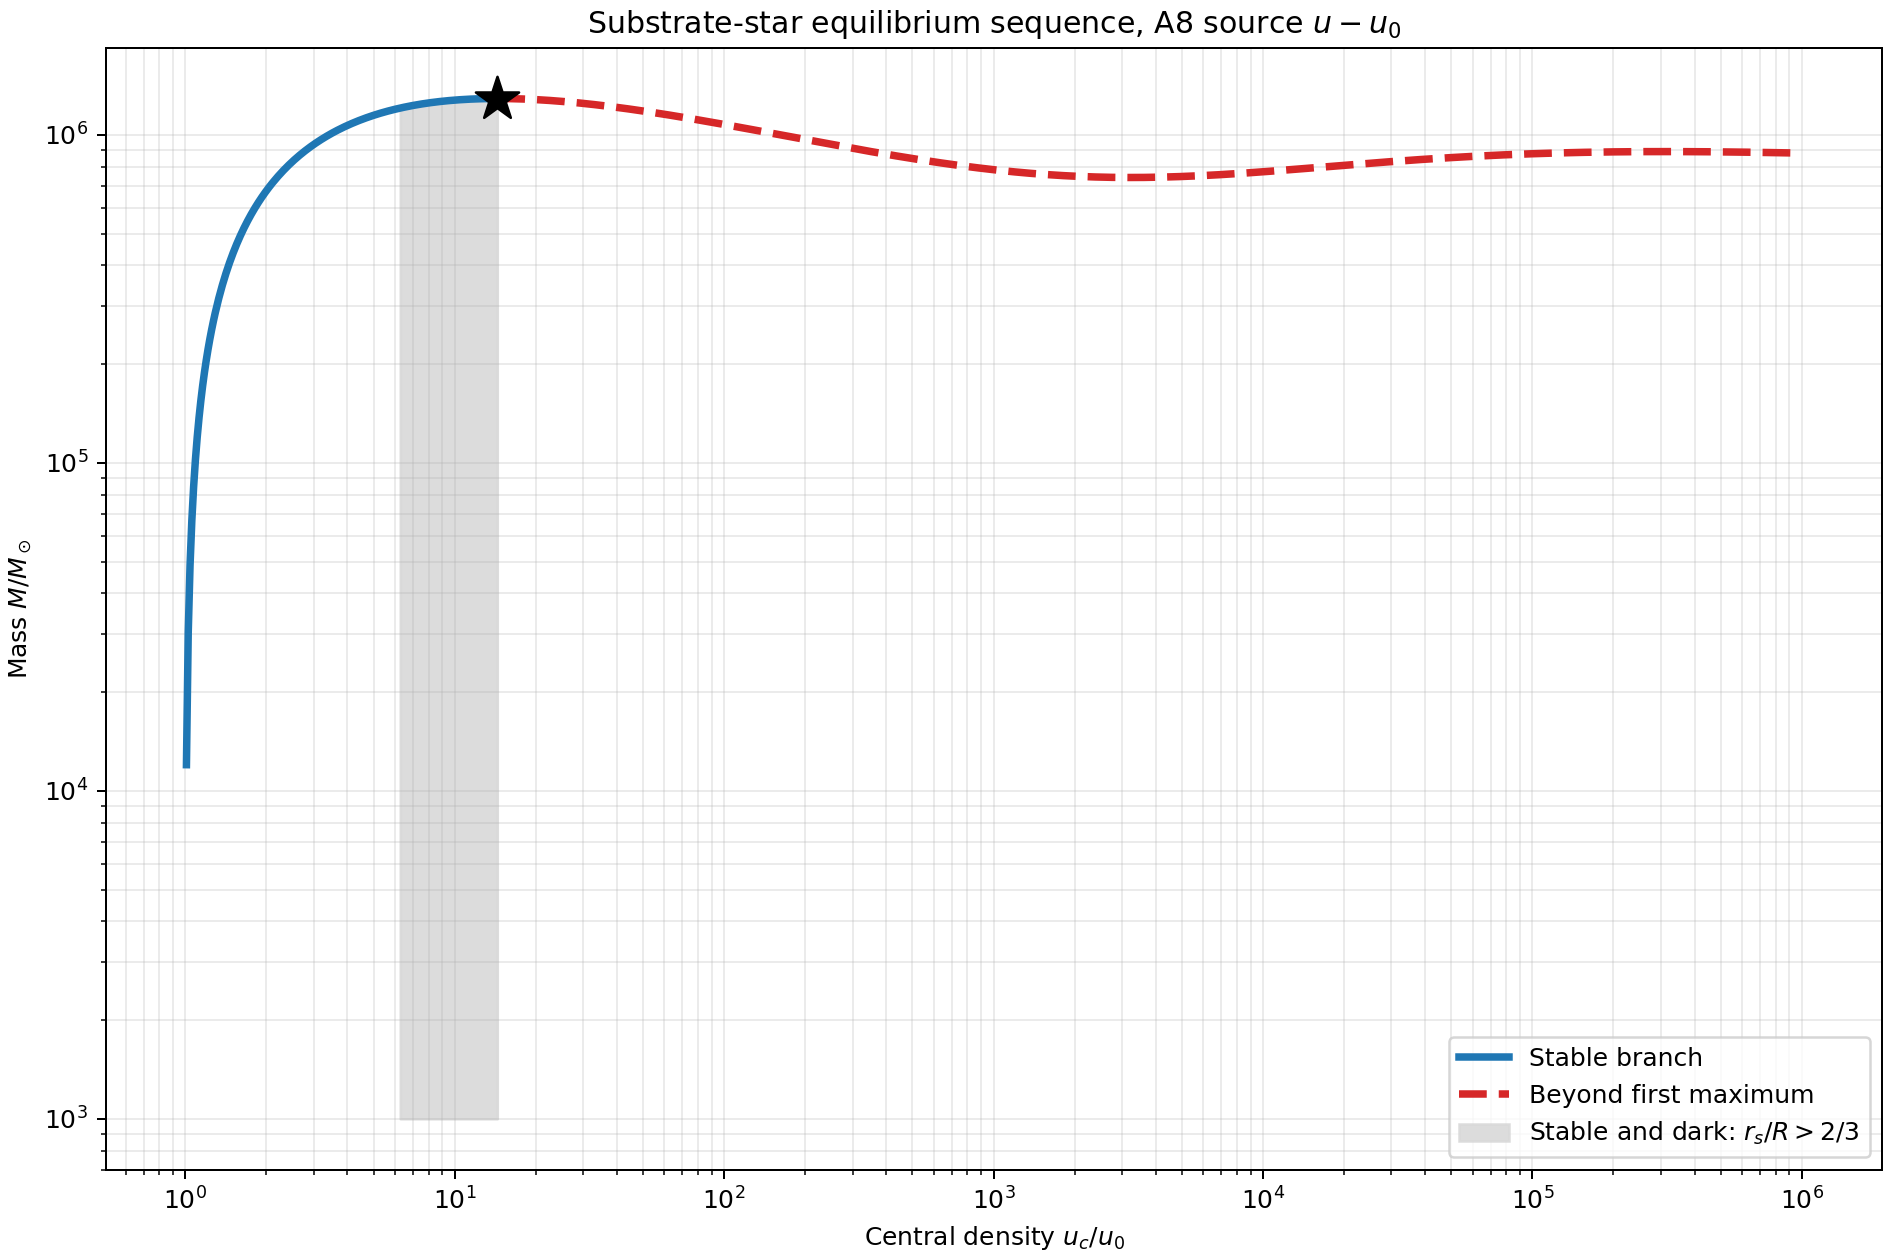
\includegraphics[width=0.82\textwidth]{fig_branch.png}
\caption{Substrate-star equilibrium sequence $M(u_c)$ from the re-integration of the system~\eqref{eq:star_structure} with the A8-consistent source $u - u_0$. The stable branch (solid) terminates at the first maximum $M_{\text{crit}} \approx 1.29\times10^{6}\,M_\odot$ ($u_c/u_0 \approx 14.5$, $r_s/R \approx 0.81$); beyond it (dashed), no equilibrium exists and collapse freezes asymptotically. The shaded region marks stable configurations that are dark with a Schwarzschild exterior ($r_s/R > 2/3$, photon sphere at $3r_s/2$ outside the surface): horizonless objects casting a shadow identical to that of a black hole.}
\label{fig:branch}
\end{figure}

\subsection{Numerical Results: Attractor, Critical Mass, and Stability}
The numerical integration of the system~\eqref{eq:star_structure} reveals three structural properties:
\begin{enumerate}
    \item \textbf{Attractor.} Beyond the critical point, solutions converge toward $M \approx 0.9\times10^{6}\,M_\odot$ at compactness $r_s/R \approx 0.68$, robustly across six orders of magnitude of central density ($r_s \equiv 2GM/c_0^2$).
    \item \textbf{Photon sphere.} With the Schwarzschild exterior of Section~\ref{sec:tensor_sector}, the photon sphere sits at $r_{\text{ph}} = 3r_s/2$. Any configuration with $R < 3r_s/2$, i.e.\ $r_s/R > 2/3$, therefore casts a shadow indistinguishable from that of a black hole: a dark object, without horizon. (For the scalar profile alone the photon sphere would sit at $r_s$; that statement is superseded.)
    \item \textbf{Stability branch.} The first-maximum criterion of $M(u_c)$ along the sequence of equilibria delimits a continuous stable branch up to a Chandrasekhar-like critical mass:
\end{enumerate}

\begin{center}
\begin{tabular}{cccc}
\toprule
$u_c/u_0$ & $M$ ($M_\odot$) & $r_s/R$ & Status \\
\midrule
$1.05$ & $5.8\times10^{4}$ & $0.02$ & stable \\
$1.9$ & $6.4\times10^{5}$ & $0.29$ & stable \\
$3.3$ & $9.8\times10^{5}$ & $0.49$ & stable \\
$5.9$ & $1.19\times10^{6}$ & $0.65$ & stable \\
$14.5$ & $\mathbf{1.29\times10^{6}}$ & $0.81$ & $M_{\text{crit}}$ (limit) --- dark \\
$>14.5$ & $< M_{\text{crit}}$ & $\sim0.7$ & unstable $\to$ freezing \\
\bottomrule
\end{tabular}
\end{center}

There thus exist \emph{stable} configurations at $r_s/R > 2/3$: stable dark objects, with a Schwarzschild shadow, without horizon or singularity, occupying the upper end of the branch ($u_c/u_0 \gtrsim 6.5$). The compactness increases monotonically along the stable branch and reaches its maximum exactly at the critical point: $\left(r_s/R\right)_{\max} = 0.81$ is the maximal compactness of any stable configuration; no stable equilibrium exists beyond it. The earlier value $1.22$, and the associated statement that stable configurations could lie \emph{inside} their own Schwarzschild radius, resulted from sourcing the field with the total $u$ in violation of Axiom~A8 and are withdrawn.

\paragraph{Scaling verification and anchor sensitivity.} The scaling $M_{\text{crit}} \propto \ell_1^2$ is verified numerically to be exact: rerunning the full integration for $\ell_1/\ell_{1,\text{nom}} \in \{0.5, 1, 1.63, 4\}$ yields $M_{\text{crit}}\,(\ell_{1,\text{nom}}/\ell_1)^2 = 1.29\times10^{6}\,M_\odot$ to all displayed digits, with the critical central density $u_c/u_0 \approx 14.5$ invariant --- as required dimensionally, the only mass scale of the system~\eqref{eq:star_structure} being $c_0^4/\sqrt{G^3 u_0} \propto \ell_1^2$. Since $\ell_1 \propto 1/m_e$, the experimental uncertainty of the anchor propagates as $\delta M_{\text{crit}}/M_{\text{crit}} = 2\,\delta m_e/m_e \approx 6\times10^{-10}$ (CODATA), entirely negligible against the modeling uncertainties (Newtonian interior, closure equation of state). Figure~\ref{fig:scaling} displays the verification.

\begin{figure}[htbp]
\centering
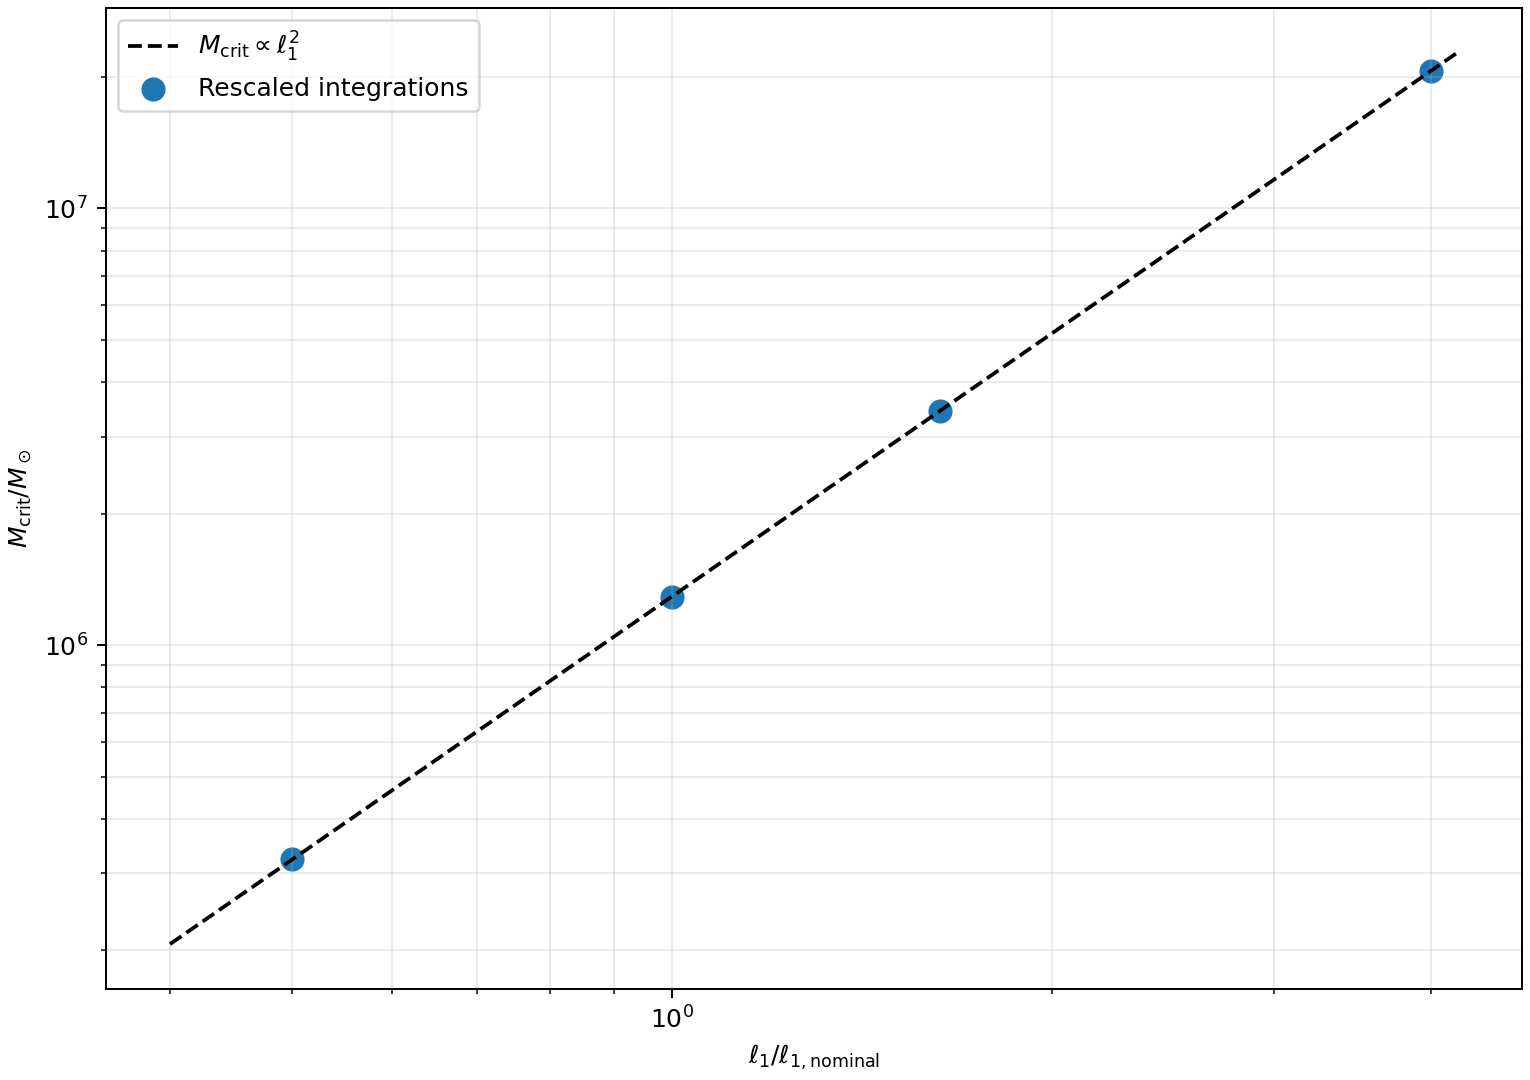
\includegraphics[width=0.7\textwidth]{fig_scaling.png}
\caption{Exact quadratic scaling of the critical mass with the string length: full numerical integrations of the system~\eqref{eq:star_structure} for $\ell_1/\ell_{1,\text{nom}} \in \{0.5, 1, 1.63, 4\}$ (points) against the law $M_{\text{crit}} \propto \ell_1^2$ (dashed). The nominal anchor gives $1.29\times10^{6}\,M_\odot$; the point at $\ell_1\times1.63$ verifies the scaling law only --- the corresponding recalibration is excluded by the thermal-surface argument (Section~\ref{sec:substrate_stars}).}
\label{fig:scaling}
\end{figure}

\paragraph{Justification of the stability criterion.} For a one-parameter sequence of equilibria with a fixed barotropic equation of state, the turning-point theorem identifies the first extremum of $M(u_c)$ with the point of marginal radial stability ($\omega_0^2 = 0$ for the fundamental pulsation mode) \cite{shapiro_teukolsky}: the static first-maximum criterion used here is therefore not merely heuristic but coincides, for this class of sequences, with the dynamical threshold. A direct computation of the radial eigenfrequencies in the DS interior --- which requires the covariant reformulation of the matter sector --- is retained among the open problems.

The critical mass obeys $M_{\text{crit}} \propto \ell_1^2$; the nominal value $\ell_1 = 8.09\times10^{-13}$~m gives $1.3\times10^{6}\,M_\odot$. The mass scale of galactic dark objects thus emerges from the substrate constants alone ($G$, $c_0$, $\ell_1$) --- a property possessed by no standard exotic compact-object model (gravastar, boson star), whose masses are free parameters \cite{mazur2001, mazur2023}. A previously entertained $\times1.63$ recalibration of $\ell_1$ (placing Sgr~A$^*$ at the critical point of the stable branch) is now \emph{excluded} by the thermal-surface argument: a stable substrate star has surface redshift $1+z = (1 - r_s/R)^{-1/2} \le 2.3$ (Schwarzschild exterior, $r_s/R \le 0.81$) and no kinematic shield; in steady state it must re-emit its full accretion power (Broderick--Narayan). This energy-conservation argument holds wherever inside the object the accreted matter comes to rest (Section~\ref{sec:lrd} and the two-component item of Section~\ref{sec:open_problems}): the location of the re-emission changes, the emitted luminosity does not. The non-detection of any thermal surface component from Sgr~A$^*$ (accretion $\sim 6\times10^{38}$~erg/s versus bolometric $\sim 10^{36}$~erg/s) forbids Sgr~A$^*$ from lying on the stable branch: $M_{\rm crit} < 4.3\times10^{6}\,M_\odot$ strictly. The nominal anchor, with Sgr~A$^*$ as a Family-3 frozen collapse, is thereby confirmed; frozen collapses themselves escape the thermal-surface test by the same kinematic freeze that silences their echoes (Section~\ref{sec:discussion}).

\subsection{Frozen Collapses: The Three Families of Dark Objects}
Outside the stable branch ($M > M_{\text{crit}}$, or stellar objects whose substrate equilibrium would be too diffuse to be dark), there is no equilibrium --- but no singularity either. The infall velocity is capped by $c_{eff} = c_0 e^{-\chi}$, which decreases exponentially during compression: the collapse \emph{freezes} asymptotically and no singularity forms in finite time. From the outside, the frozen object is optically indistinguishable from a black hole (practically divergent redshift, Schwarzschild shadow and orbits). The model therefore predicts three families:
\begin{itemize}
    \item \textbf{Family 1} --- stellar objects (X-ray binaries, LIGO mergers): frozen collapses;
    \item \textbf{Family 2} --- $\sim10^{4}$ to $1.3\times10^{6}\,M_\odot$: substrate stars in stable equilibrium (the only family possessing a true surface); dark only above $r_s/R = 2/3$;
    \item \textbf{Family 3} --- supermassive $> M_{\text{crit}}$ (Sgr~A$^*$ marginal, M87$^*$): frozen collapses.
\end{itemize}
A distinctive prediction of principle: the surface redshift is enormous but finite --- a residual radiative leakage exists, exponentially suppressed, qualitatively distinct from GR.

\subsection{Debts of the Calculation}
The treatment of momentum is Newtonian, marginal at compactness $\sim1$ (a covariant reformulation of the matter--substrate sector is required; the conformal representative of the coupling is now fixed, Section~\ref{sec:conformal_representative}); stability is assessed by the static criterion only; the hypothesis $E = hc_0/\ell$ per cell under compression is a closure postulate; the interior is integrated for the substrate \emph{alone}, without an ordinary-matter component, although an accreting object necessarily contains one (the two-component problem, Sections~\ref{sec:lrd} and~\ref{sec:open_problems}); finally, the shear-wave absorption condition at the surface (Section~\ref{sec:discussion}) remains undemonstrated.

% =====================================================
% PART III : QUANTUM UNIFICATION AND KINEMATICS
% =====================================================
\part{Kinematics of Media}

\section{Quantum Correlations: Scope and Withdrawals}
\label{sec:nonlocal_correlations}

\subsection{Differential-Mode Phase Opposition: Conditional Scope}
Two identical resonant circuits coupled through a reactive network admit common and differential normal modes. A phase difference of $\pi$ is therefore a legitimate \emph{conditional} differential-mode solution once the sign and strength of the mutual coupling are specified. The DS manuscript uses this circuit fact in the hydrogen discussion. It does not, however, derive that particle--antiparticle creation selects this mode, that the mode persists as the defects separate, or that it represents a non-separable quantum state. The former ``phase-opposition pair postulate'' is consequently reclassified as a phenomenological ansatz rather than a mechanism of pair creation.

\subsection{Withdrawal of the Low-Impedance Corridor}
Earlier versions introduced a compressed, low-impedance wake between separated defects and assigned it a synchronization speed $v_{\rm sync}=c_0 Z_0/Z_{\min}$. No field equation, constitutive law, or conservation argument in the model yields that relation. Axiom~A5 only forbids pole fusion; it does not determine a wake geometry, an impedance floor, or a propagation law. The numerical inferences formerly drawn from Bell tests --- bounds on $Z_{\min}$ and on a separation $D-2r$ --- were therefore consequences of an assumed formula rather than predictions. They are withdrawn.

\subsection{Entanglement and Measurement: No Present Mechanism}
Experimentally observed Bell correlations are described in quantum theory by a joint non-separable state. The present DS construction neither derives such a state from its DQD degrees of freedom nor supplies a probability rule connecting those degrees of freedom to measurement outcomes. Topological connection by itself is insufficient: a classical shared circuit can generate correlations but cannot reproduce the quantum statistics without additional non-local or contextual structure. Conversely, importing an Anderson--Higgs analogy does not close the gap. A finite-energy charged vortex requires a genuine charged order parameter and a gauge-covariant kinetic term; the telegrapher flux is an electromagnetic circuit variable and is not automatically a Higgs field. No independent condensate density, kinetic inductance, London length, or coherence length is presently defined in the DS model.

Accordingly, this section makes no claim to explain Bell correlations, collapse, decoherence, or the Born rule. Any future microscopic proposal must state its dynamical variables, Hamiltonian or action, gauge structure, initial-state preparation, and measurement map, then reproduce the quantum probabilities while respecting operational no-signaling. Until that calculation exists, entanglement is inherited from standard quantum mechanics as an empirical constraint on the model, not explained by a sub-vacuum communication channel.

\section{Lorentz Invariance as an Emergent Symmetry of the Substrate}
\label{sec:lorentz}

The present formalism is of the Lorentz-ether type \cite{einstein1920}: length contraction and time dilation follow as exact electrodynamic and hydrodynamic consequences of an oscillating circuit progressing through the DQD gas, in place of the geometric postulate that treats them as intrinsic properties of spacetime.

The mechanism underlying this section --- an autonomous localized excitation of a discrete classical medium acquiring relativistic kinematics, an internal clock obeying $\omega' = \omega_0/\gamma$, and an inertial mass equal to $E/c^2$ --- now has a numerical proof of principle: Appendix~\ref{app:breathers} shows that a sub-gap breather on a discrete sine-Gordon lattice recovers all these relations in the continuum limit, with deviations measured to converge at second order in the mesh, and that the closure holds only for the autonomous object (a pumped excitation phase-locked to an external clock does not close, \S\ref{app:breathers_open}). This is a proof of mechanism on a surrogate lattice, not a validation of the DQD substrate: the numerical demonstration establishes that the medium-based route to relativistic kinematics is viable in a locally coupled classical system, and nothing more.

\subsection{The Heaviside Ellipsoid and Convective Impedance}

At rest, a matter soliton generates an isotropic spherical impedance profile $Z(r) = Z_0 \exp(2GM/rc_0^2)$. When a soliton ($\Ncd \ge 3$) moves at constant velocity $v$ along the $x$ axis, it experiences the dynamic pressure of the substrate. The polarization field of the lattice no longer propagates isotropically, but undergoes longitudinal compression.

The effective radial distance perceived by the lattice dynamics becomes a convective radius $r^*$, modulated by the elastic Lorentz factor $\gamma = (1 - v^2/c_0^2)^{-1/2}$:
\begin{equation}
r^* = \sqrt{\gamma^2 x^2 + y^2 + z^2}
\end{equation}

The dynamic impedance of the moving particle flattens into a Heaviside ellipsoid, drastically increasing the reactive energy density on the transverse axis:
\begin{equation}
Z_{mvt}(x,y,z) = Z_0 \exp\left( \frac{2GM}{c_0^2 \sqrt{\gamma^2 x^2 + y^2 + z^2}} \right)
\end{equation}

\emph{Verification, and its exact scope (revised).} Applied to this convective profile, the \emph{flat} wave operator $\nabla^2\chi - c_0^{-2}\partial_t^2\chi$ has an identically null residual (computer algebra). This is a genuine result, but it does not say what earlier versions claimed: the flat operator is not the field equation of the Lagrangian~\eqref{eq:lagrangian}, which is the nonlinear Eq.~\eqref{eq:true_field_eq}. Substituting the convective profile into the true field equation leaves a residual that is \emph{second order} in the field: writing $\chi = A/r^*$, the residual scales as $A^2$ (verified numerically over three decades in $A$, the ratio residual$/A^2$ being constant to four digits) and grows monotonically with $v$. The correct statement is therefore: \emph{the Heaviside ellipsoid is an exact solution of the linearized dynamics, with a violation of the full field equation of order $\chi^2$}. This does not affect the static extraction of $\gamma = \beta = 1$, which is read off the exterior isotropic metric and does not use the convective profile; its consequences for moving-frame post-Newtonian terms remain open (Section~\ref{sec:open_problems}). We note explicitly that the $O(\chi^2)$ order is not \emph{a priori} negligible for the post-Newtonian comparison, since $\beta$ is itself read from the $U^2$ coefficient of $g_{00}$; the point is that the static determination does not pass through this profile, not that the order is too small to matter. The ellipsoid is a first-order consequence of the scalar sector, not an exact one, and the earlier claim of exactness is withdrawn.

\begin{figure}[htbp]
\centering
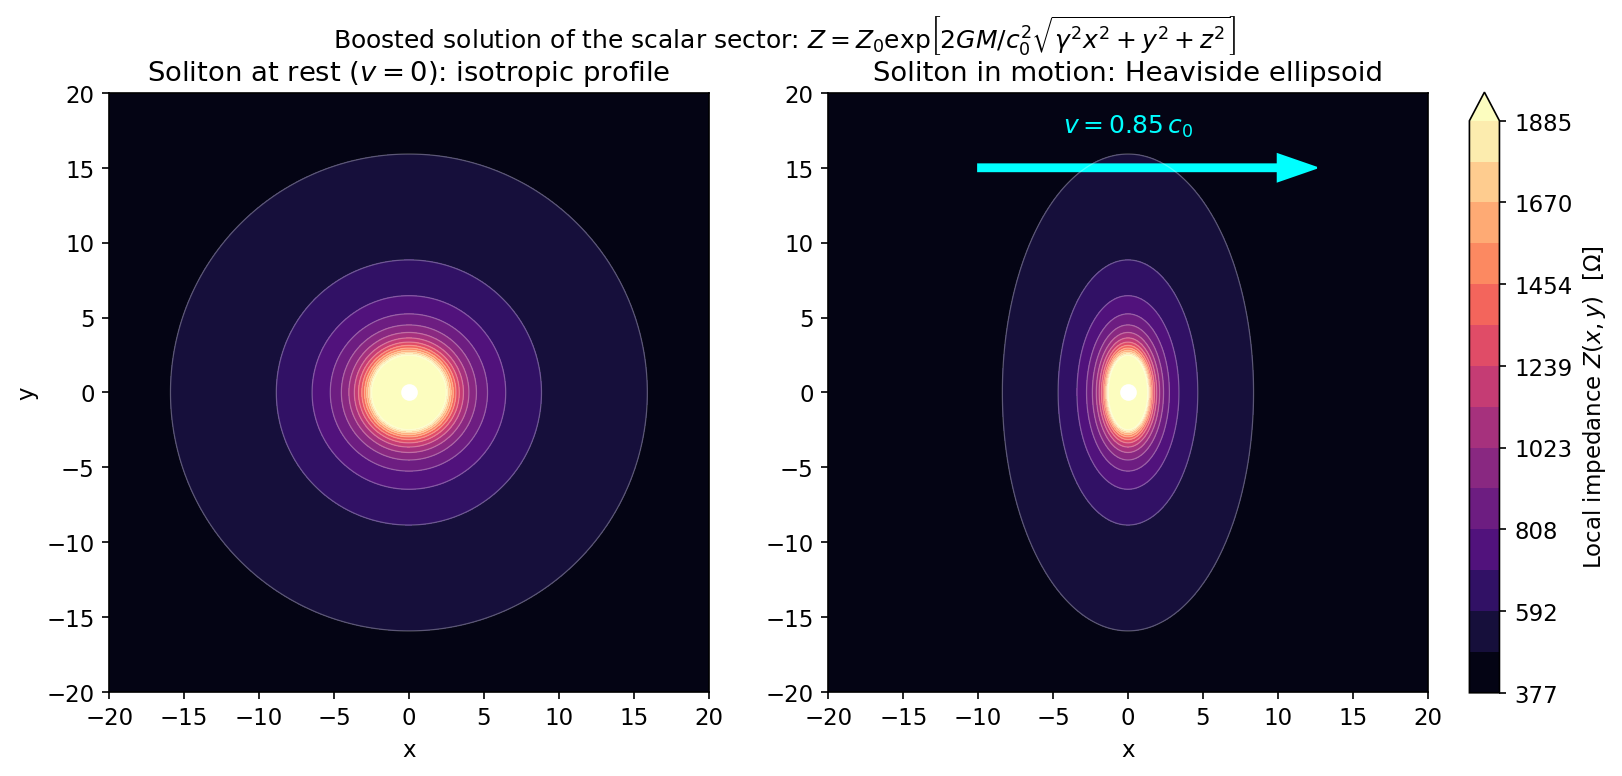
\includegraphics[width=0.95\textwidth]{fig_heaviside.png}
\caption{Impedance field of a soliton at rest (left, isotropic exponential profile) and in uniform motion at $v = 0.85\,c_0$ (right): the equal-impedance surfaces contract into the Heaviside ellipsoid, $Z = Z_0\exp[2GM/c_0^2\sqrt{\gamma^2x^2+y^2+z^2}]$. This profile is an exact solution of the linearized scalar dynamics; its residual in the full nonlinear field equation is $O(\chi^2)$ (Theorem~3).}
\label{fig:heaviside}
\end{figure}

To formalize this structural adaptation, we posit a new fluid-dynamics axiom:

\begin{description}
\item[A6 --- Heaviside Convective Equilibrium.] Any soliton ($\Ncd \ge 3$) in stationary motion at velocity $v$ mechanically adjusts its internal geometry so that its structural impedance $Z_{topo}$ remains locally matched to the convection flux of the DQD substrate. This pressure produces a physical contraction of the particle by a factor $\gamma$ along the direction of motion.
\end{description}

\subsection{Clock Slowing by Inductive Overload}

In this framework a clock (or an atom) is a $c_0$-confined standing wave: the soliton is a wave folded on itself at the quantization condition $\beta\ell = p\pi$ (Section~\ref{sec:impedance_confinement}). Its tick is therefore a light-clock, and its slowing under motion follows from geometry alone, with no malleable ``time'' postulated.

Work in the substrate rest frame, where all internal signals propagate at $c_0$. A transverse internal cycle (perpendicular to the motion) of a soliton of radius $R$ traverses the Pythagorean path
\begin{equation}\label{eq:tperp}
t_\perp = \frac{2R}{c_0}\,\gamma,
\end{equation}
the standard light-clock result. For the \emph{longitudinal} cycle the outcome depends on whether the soliton contracts. Without contraction, the back-and-forth along the direction of motion gives
\begin{equation}\label{eq:tpar_nocontract}
t_\parallel = \frac{2R}{c_0}\,\gamma^2,
\end{equation}
so that $t_\parallel \neq t_\perp$: the internal clock would be \emph{anisotropic}, ticking at different rates along and across the motion --- an observable directional dependence of atomic frequencies, excluded experimentally. Imposing isotropy $t_\parallel = t_\perp$ forces the longitudinal radius to contract as $R \to R/\gamma$, which is exactly Axiom A6 (Heaviside convective equilibrium). With A6 the longitudinal cycle becomes
\begin{equation}\label{eq:tpar_contract}
t_\parallel = \frac{2R}{c_0}\,\gamma,
\end{equation}
matching Eq.~\eqref{eq:tperp}. The internal resonance frequency of the moving soliton therefore drops isotropically as
\begin{equation}
\omega' = \frac{\omega_0}{\gamma},
\end{equation}
and A6 follows as the condition that the soliton's light-clock remain isotropic --- the same argument by which FitzGerald and Lorentz were historically forced to length contraction --- rather than standing as an independent postulate. The same dilation law is recovered numerically, without any imposed geometry, by the internal clock of an autonomous lattice breather ($\omega_b = \omega_{b0}/\gamma$ to $\le 0.3\,\%$ at the finest boosted resolutions, Appendix~\ref{app:breathers}). As a corollary, the reactive time constant obeys $\tau \propto \sqrt{L'C'} = \gamma\sqrt{LC}$: the effective $\sqrt{LC}$ dilation emerges as a \emph{consequence} of the light-clock.

\paragraph{Impedance and geometry are one clock.} The light-clock and the reactive descriptions of the slowing are the same statement read two ways. The convective compression concentrates the transverse flux lines, raising the cavity inductance by $L \to \gamma^2 L$ while the capacitance stays rigid ($C \propto \rho^0$, Section~\ref{sec:kinematic_gravity}); the reactive period then dilates exactly as $\tau = \sqrt{L'C'} = \gamma\sqrt{LC}$, the cavity impedance rises as $Z_{\text{topo}} \to \gamma\,Z_{\text{topo}}$, and the internal celerity falls as $1/\gamma$ --- the confined $c_0$-wave takes $\gamma$ times longer to close its loop. This is the moving clock of the light-clock argument, now expressed through the impedance the soliton presents to the substrate. (The $Z$ that carries the clock is the \emph{internal} cavity impedance $Z_{\text{topo}}$, not the external gravitational profile $Z(r)$ of Eq.~\ref{eq:lagrangian}\,ff.; time dilation is therefore mass-independent, as required --- an electron and a proton at the same $v$ share the same $\gamma$.) The earlier reading in which $L$ rose by a single factor $\gamma$ is superseded: it would give $\tau \propto \gamma^{1/2}$ and hence $\omega' = \omega_0/\sqrt\gamma$, whereas the light-clock and the $\gamma^2$ inductance compression both yield $\omega' = \omega_0/\gamma$.

In the limit $v \to c_0$ the internal clock stops ($\gamma \to \infty$): only unfolded topologies (no loop, hence no internal clock --- $\Ncd = 1,2$) can reach $c_0$, consistently with the massless-particle table of Appendix~B.

The slowing of comoving clocks is thus a pure causal-geometry effect: the internal engine of the particle, being itself a $c_0$-confined wave, cannot tick faster than its own folded light path allows.

\subsection{Demonstration of Emergent Covariance}

Consider an interferometer of proper rest length $L_0$, traveling at velocity $v$. By virtue of Axiom A6, the standard rod physically contracts according to the exact law $L' = L_0/\gamma$. The absolute round-trip time of light in the instrument writes:
\begin{equation}
t_{tot} = \frac{L'}{c_0 - v} + \frac{L'}{c_0 + v} = \left(\frac{L_0}{\gamma}\right) \frac{2c_0}{c_0^2(1 - v^2/c_0^2)} = \frac{2L_0}{c_0} \cdot \gamma
\end{equation}

Simultaneously, the local clock of the observer, subject to the inductive overload of the medium, ticks at a rate slowed by a factor $\gamma$. The local time $t'$ displayed by the comoving apparatus will therefore be:
\begin{equation}
t' = \frac{t_{tot}}{\gamma} = \frac{2L_0}{c_0}
\end{equation}

Any local measurement of the speed of light ($c_{measured}$) performed with this contracted rod and this slowed clock will invariably return the nominal celerity of the substrate:
\begin{equation}
c_{measured} = \frac{2L_0}{t'} = c_0
\end{equation}

The undetectability of the preferred frame expresses a theorem of perfect elastic equilibrium within the DQD gas, with the laws of classical kinematics left intact.

\section{Stability of the Substrate}
\label{sec:dynamic_balance}

\paragraph{Purpose.} This section records the stability analysis of the substrate. It establishes two constraints having the status of theorems, deduces from them the gaseous nature of the medium, and formalizes the two dynamical axioms (A4, A5) required by the consistency of the whole model.

\subsection{Stability Constraints}

\begin{thmA}
No static configuration of DQDs maintained by the Coulomb interaction of their poles alone is mechanically stable. An electrostatic potential being harmonic ($\nabla^2 V = 0$), it possesses no local minimum (Earnshaw's theorem). \textbf{Consequence:} the fluctuating character of the substrate is not a descriptive choice but a necessity.
\end{thmA}

\begin{thmB}
The substrate cannot condense into a self-bound liquid. The zero-point confinement energy of a massless DQD ($E_{\text{conf}} \sim \pi\hbar c_0/\ell$) and the dipolar cohesion energy ($E_{\text{coh}} \sim \tfrac{2}{9}\alpha\,\hbar c_0/\ell$) both decrease as $1/\ell$; their ratio is therefore constant:
\begin{equation}
\frac{E_{\text{conf}}}{E_{\text{coh}}} = \frac{9\pi}{2\alpha} \approx 1937 .
\end{equation}
The confinement pressure dominates the cohesion by three orders of magnitude at any density; binding would require $\alpha > 9\pi/2 \approx 14$. \textbf{Consequence:} the stability of the vacuum against self-condensation is guaranteed by the smallness of the fine-structure constant.
\end{thmB}

\paragraph{Gaseous nature and stability of $\alpha$.} Theorems~1 and~2 impose that the substrate be a gas of free DQDs propagating isotropically at $c_0$. The density $\rho_0$, hence $\ell_{\text{cell}} \equiv \nu^{-1/3}$, is there an initial condition and not a quantity fixed by a local equilibrium. A uniform, infinite gas does not dilute (any outflow from a region is statistically compensated): the density remains constant, ensuring the constancy of $Z_0$, hence of $\alpha = e^2 Z_0/2h$, in agreement with the spectroscopic constraints on the variation of $\alpha$ ($|\Delta\alpha/\alpha| < 10^{-5}$ over the age of the Universe).

\paragraph{Cosmological scope note.} The constancy argument of this section (a uniform infinite gas does not dilute) is incompatible with metric expansion, which is independently required by SN~Ia light-curve time dilation $\propto (1+z)$, by $T_{\rm CMB}(z) = T_0(1+z)$, and by primordial nucleosynthesis. Cosmological evolution therefore lies outside the model's scope; where Section~\ref{sec:lrd} uses redshifts and distances, it does so on the standard cosmology. A $\rho_0(t)$ history preserving both the constancy of $\alpha$ and the epoch-independence of $\ell_{\rm cell}$ is an open problem.

\subsection{Dynamical Axioms}

\begin{description}
\item[A4 --- Matching principle.] The sub-vacuum dynamics relaxes toward impedance matching: the substrate locally minimizes $|\Gamma|^2$. This relaxation law --- and not an electrostatic equilibrium --- confers on the configuration $\Gamma_{\text{bif}}(D_0)=0$ the status of a stable attractor, thereby escaping the Earnshaw exclusion (Theorem~1).
\item[A5 --- Topological rigidity of the DQD.] The DQD possesses no continuous deformation mode. Its only accessible transition is the discrete switch to the micro-loop configuration (neutrino), transient and quantized. The poles of distinct strings do not merge, which forbids the spontaneous condensation of the vacuum into matter. This axiom justifies treating the DQD as a rigid object in the impedance calculations (Section~\ref{sec:impedance_confinement}) and grounds the origin of $\varepsilon_0$ as an orientational response of the gas, without internal deformation. \emph{Reading:} A5 plays here the role that a short-distance regularization plays in any continuum theory containing point singularities --- without it, the pole--pole interaction diverges at contact and the impedance calculations are ill-posed. It is therefore not an arbitrary rigidity clause but the statement that the continuum description must be completed below the string radius.
\end{description}

\subsection{$\mathcal{R}$ as a Derivation Target}

In the light of axioms A4 and A5, the three terms of the unified ansatz (Eq.~\ref{eq:additive_ansatz_expanded}) appear as the three regimes of a single law: the fluctuation amplitude of the DQDs adjusts to the local impedance of the traversed medium.

\begin{center}
\begin{tabular}{lll}
\toprule
\textbf{Term of $\mathcal{R}$} & \textbf{Regime} & \textbf{Microscopic brick to derive} \\
\midrule
$Z_{\text{base}}(1+2GM/|x|c_0^2)$ & Refractive gravity & Gas compression (Sec.~\ref{sec:kinematic_gravity}, derived) \\
$\Delta Z(\vec{\Pi},\varepsilon_{\text{eff}})$ & Dielectric response & Orientational statistics $\langle p^2\rangle$ of the gas \\
$-Z_{\text{base}}\,\beta_{\text{vtx}}^2$ & Vorticity & Proper rotation statistics of the cells \\
\bottomrule
\end{tabular}
\end{center}

\paragraph{Epistemological status.} No new numerical value --- notably $\ell_{\text{cell}}$ --- reaches the \emph{Derived} level at the end of this analysis: the attempted dielectric closures proved dependent on a modeling convention for the deformed impedance, not decided by the current formalism. The acquired result is \emph{structural}: the transformation of $\mathcal{R}$ from a postulated ansatz into a target of microscopic derivation whose missing bricks are explicitly inventoried.

\section{Electrodynamic Synthesis: Unified Impedance Ansatz}
\label{sec:electrodynamic_synthesis}

\subsection*{Epistemological note}
The following equation constitutes a first-order phenomenological ansatz. Contrary to the earlier multiplicative approaches, this formalism postulates that each interaction layer (geometric, dielectric, gravitational, and hydrodynamic) articulates as an additive superposition of contributions or electrodynamic potentials defining the state function of space, denoted $\mathcal{R}$:

\begin{equation}
\label{eq:additive_ansatz_global}
\boxed{R(Z, \Pi, \omega, x) = Z(C, L, x) + \Pi(\vec{\Pi}, \epsilon_{\text{eff}}, x) + \Omega(\omega, \ell_{\text{cell}}, x)}
\end{equation}

Each component of this sum is defined at every point $x$ of the lattice by:
\begin{itemize}
    \item \textbf{The structural impedance} $Z(C, L, x)$: it describes the base lattice of the vacuum (linked to the inductance $L_0$ and capacitance $C_0$), modulated at first order by the refractive-metric solution at position $x$:
    \begin{equation}
    Z(C, L, x) = Z_{\text{base}} \exp\left(\frac{2GM}{|x|c_{0}^{2}}\right)
    \end{equation}
    \item \textbf{The polarization component} $\Pi(\vec{\Pi}, \epsilon_{\text{eff}}, x)$: it expresses the local modification of the dynamic dielectric permittivity of the substrate $\epsilon_{\text{eff}}$ under the effect of the complex polarization vector field $\vec{\Pi}$:
    \begin{equation}
    \Pi(\vec{\Pi}, \epsilon_{\text{eff}}, x) = \Delta Z(\vec{\Pi}, \epsilon_{\text{eff}})
    \end{equation}
    \item \textbf{The vorticity component} $\Omega(\omega, \ell_{\text{cell}}, x)$: it introduces the kinematic correction linked to the rotation of the DQD cells via the vorticity field $\omega$ and the local cell size $\ell_{\text{cell}}$. This contribution acts purely subtractively via the normalized tangential velocity factor $\beta_{\text{vtx}}$:
    \begin{equation}
    \Omega(\omega, \ell_{\text{cell}}, x) = - Z_{\text{base}} \left(\frac{\ell_{\text{cell}}^{2}|\omega|^{2}}{c_{0}^{2}}\right) = - Z_{\text{base}} \beta_{\text{vtx}}^{2}
    \end{equation}
\end{itemize}

In its expanded, first-order-linearized form, the unified additive ansatz writes:
\begin{equation}
\label{eq:additive_ansatz_expanded}
R(Z, \Pi, \omega, x) = Z_{\text{base}}\left(1 + \frac{2GM}{|x|c_{0}^{2}}\right) + \Delta Z(\vec{\Pi}, \epsilon_{\text{eff}}) - Z_{\text{base}}\beta_{\text{vtx}}^{2}
\end{equation}
where $\beta_{\text{vtx}} = \ell_{\text{cell}}|\omega|/c_{0}$ is the normalized vortex velocity factor, strictly bounded in $[0,1[$, expressing the sub-luminal regime of the substrate.

This additive formulation exhibits the vorticity wake as a subtractive term: within the ansatz, a strong vorticity ($\omega$) lowers the local impedance ($Z < Z_0$) and changes the effective propagation speed sampled by the Pump--Probe protocol (whose experimental phenomenology is the subject of Section~\ref{sec:discussion}). Whether this effective-medium parameter can exceed its vacuum value without conflict with front-velocity causality is not established by the scalar ansatz.

\subsection{Scale Distinction of the Reflection Coefficients}
To avoid any ambiguity on the stability of the lattice reorganized in additive form, we make explicit that the model involves two reflection coefficients operating at distinct physical scales:
\begin{itemize}
    \item \textbf{The sub-vacuum interface coefficient ($\Gamma_{\text{pole}}$):} fixed at $\Gamma_{\text{pole}} = 1/3$, it qualifies the local geometric rupture between the unit string ($Z_{\text{half\_dqd}} = Z_{0}/2$) and the surrounding fluid at rest ($Z_{0}$). It is an intrinsic structural property of the interface at the sub-causal scale, guaranteeing the nominal equilibrium spacing of the cell.
    \item \textbf{The dynamic line coefficient ($\Gamma_{\text{bif}}(D)$):} it governs the complete DQD cell facing the macroscopic vacuum under an external mechanical constraint. When the spacing $D$ tends toward the core diameter $2r$, the line impedance collapses ($Z_{\text{bif}} \rightarrow 0$), driving this coefficient toward total short-circuit mismatch ($|\Gamma_{\text{bif}}| \rightarrow 1$) and triggering the stationary restoring force.
\end{itemize}

\subsection{Mechanism of Reactive Confinement Pressure}
The restoring force exerted on the walls of the DQD under compression is a reactive confinement pressure, distinct from classical radiation pressure (which is associated with a propagating flux dictated by a Poynting vector). It is interpreted as the direct analogue of the mechanical force exerted on the internal walls of an energized inductor when its geometry is perturbed: the compression of the dielectric micro-cavity neither absorbs nor dissipates active power, and instead compresses the stationary reactive energy density stored sub-vacuum. The surge of counter-pressure is the macroscopic consequence of this purely reactive energy flux opposing the modification of its confinement geometry.

\subsection{Intrinsic Limitations of the First-Order Ansatz}
As an engineering conjecture, this additive unified ansatz has three major theoretical limits that mark out the model's future developments:
\begin{enumerate}
    \item \textbf{Resolution of the gravitational circularity}: The introduction of the term $Z_{\text{base}}$ in the various components implies an implicit dependence on the background impedance $Z_{0}$. In the weak field, to avoid any mathematical circularity, this coupling must be treated strictly as a linear relative correction of the refractive metric applied to the base impedance:
    \begin{equation}
    R(Z, \Pi, \omega, x) \approx Z_{\text{base}} \cdot \left(1 + \frac{2GM}{|x|c_{0}^{2}} + \mathcal{O}\left(\frac{GM}{|x|c_{0}^{2}}\right)^{2}\right) + \Delta Z(\vec{\Pi}, \epsilon_{\text{eff}}) - Z_{\text{base}} \beta_{\text{vtx}}^{2}
    \end{equation}
    \item \textbf{Absence of cross-coupling terms}: The purely additive independence of Eq.~\eqref{eq:additive_ansatz_global} neglects second-order interactions. In a complete hydrodynamic model, the cell compression induced by the gravitational gradient ($\delta \ell_{\text{cell}}$) locally modifies the fluid velocity profile, which should generate a geometry/vorticity cross term of the type $\delta(\ell_{\text{cell}}) \cdot |\omega|^{2}$. The omission of this term limits the current ansatz to weak-coupling regimes.

    \item \textbf{Scalar character of the ansatz:} The state function defined by Eq.~\eqref{eq:additive_ansatz_global} is scalar, each component contributing in norm to the effective impedance. Yet the fields $\vec{\Pi}$ and $\vec{\omega}$ define preferred directions in the lattice: a polarized or rotating substrate is intrinsically anisotropic, and its impedance then depends on the polarization of the probe wave. The complete description requires promoting $R$ to an impedance tensor (the polarization term carries the factor $Z_{\text{base}}$, by symmetry with the vorticity term, ensuring homogeneity in ohms):
\begin{equation}\label{eq:impedance_tensor}
R_{ij}(x) = Z(x)\,\delta_{ij}
  \;+\; a\,Z_{\text{base}}\,\Pi_i \Pi_j
  \;-\; b\,Z_{\text{base}}\,
        \frac{\ell_{\text{cell}}^{2}\,\omega_i\,\omega_j}{c_{0}^{2}}
\end{equation}
whose trace restores the isotropic scalar ansatz at first order, while the anisotropic terms ($\propto \Pi_i\Pi_j$, $\omega_i\omega_j$) generate two distinct eigen-impedances according to the polarization axis --- that is, a birefringence of the vacuum, precisely the observable targeted by the PVLAS and BIREF@HIBEF programs (Section~\ref{sec:discussion}). The current scalar formulation is thus limited to isotropic regimes or polarization averages.
\end{enumerate}

\subsection{Derivation of the Saturation Coefficient and Atomic Repulsion}
\label{sec:atomic_repulsion}

\paragraph{Saturation coefficient.} The coefficient $a$ of the impedance tensor is no longer free: each DQD cell carries a maximal dipole $p_{\max} = (e/3)\,D_0$ at density $1/\ell_{\text{cell}}^3$, whence the saturation polarization and the coefficient that follows:
\begin{equation}\label{eq:pi_sat}
\Pi_{\text{sat}} = \frac{(e/3)\,D_0}{\ell_{\text{cell}}^3}, \qquad a = \frac{1}{\Pi_{\text{sat}}^2}
\qquad \left(\Pi_{\text{sat}} \approx 2.4\times10^{4}~\text{C/m}^2 \;\text{for}\; \ell_{\text{cell}} = \ell_1\right).
\end{equation}
With the corrected tensor form (factor $Z_{\text{base}}$), full saturation ($|\vec{\Pi}| = \Pi_{\text{sat}}$) produces an order-unity mismatch ($\delta Z \sim Z_{\text{base}}$), the physically expected behavior. This derivation is \emph{conditional} on $\ell_{\text{cell}}$, the missing brick inventoried in Section~\ref{sec:dynamic_balance}.

\paragraph{Mechanism and scale of the atomic wall.} The reactive wall $\Gamma_{\text{bif}} \to 1$ operates at $\sim 2\times10^{-14}$~m: it cannot explain atomic impenetrability at $10^{-10}$~m. The mechanism at the right scale is \textbf{chirality frustration}: when two saturated electronic clouds overlap, the anti-parallel nesting of the tubes becomes impossible (the mechanical analogue of Pauli exclusion), the net $|\vec{\Pi}|^2$ grows with the overlap, $Z$ rises, and the stored reactive energy penalizes interpenetration. This regime is precisely the \emph{non-adiabatic} regime of the criterion of Section~\ref{sec:adiabaticity}: the $Z$ peak is steep at the very scale of the orbital mode probing it ($L_Z \sim \lambda$), forbidding retuning and forcing reflection. Two numerical bounds fix the scale of the mechanism: drawing the substrate cell energy ($E_1 \approx 1.53$~MeV per cell) would yield $\sim10^{11}$~eV per atomic overlap (eleven orders of magnitude too strong); Compton-scale field tails would yield a factor $e^{-259}$ at 1~\AA{} (mechanism extinguished). The only coherent closure: the atomic electron being a resonant cavity mode (Section~\ref{sec:kinematic_gravity}) spread at the Bohr scale, its field $\vec{\Pi}$ carries the extension and the exponential decay \emph{of the orbital mode}. Range and magnitude ($\sim$\AA, $\sim$eV) then follow the orbital energetics --- structurally isomorphic to Born's exchange repulsion. The substrate supplies the \emph{mechanism}, the orbital supplies the \emph{scale}. The binding case is obtained with no extra ingredient: when the anti-parallel nesting is possible (non-saturated orbitals), $\vec{\Pi}$ locally vanishes, no penalty appears, and the mutual-inductance coupling supplies the attraction --- an emergent Lennard-Jones-type potential.

\paragraph{Consistency clause $\chi_{\text{vac}} \ll 1$.} If the free vacuum responded with the full saturation polarizability~\eqref{eq:pi_sat}, a Petawatt laser ($E \approx 9\times10^{14}$~V/m) would produce $\delta Z/Z \sim 5\,\%$, in contradiction with PVLAS and with the estimate $\delta Z/Z \sim 10^{-6}$ of Section~\ref{sec:discussion}. The model therefore rigorously distinguishes: the dynamic susceptibility of the free vacuum, $\chi_{\text{vac}} \ll 1$ (ordered phase, rigid PLL, quasi-frozen dipoles --- grounded by the nematic order of Section~\ref{sec:tensor_sector}), and the field $\vec{\Pi}$ carried by matter, saturated by construction in the tubes.

\subsection*{Epistemological status of the results}
This working formalism distinguishes six levels of theoretical maturity:
\begin{itemize}
    \item \textbf{Derived (Predictive):} the universal geometric ratio $D/r = 2\cosh(\pi)$; the interface coefficient $\Gamma_{\text{pole}} = 1/3$; the weak-field Schwarzschild refractive index; the exact covariance identity of the scalar sector (Theorem~3; the vanishing of the preferred-frame parameters is \emph{not} claimed, see Section~\ref{sec:open_problems}); the first post-Newtonian parameters $\gamma = \beta = 1$ (Section~\ref{sec:ppn}); the numerical selection of the force law~\eqref{eq:force_law}; the identity between this law and the static geodesic of the isotropic conformal representative (Section~\ref{sec:conformal_representative}); the substrate-star branch with $M_{\text{crit}} \approx 1.3\times10^{6}\,M_\odot \propto \ell_1^2$ and maximal compactness $r_s/R = 0.81$ (A8-consistent source); the self-consistency $t_{\rm freeze} \simeq \Delta t_{\rm echo}/2$ of frozen collapses, which holds with a Schwarzschild exterior (Section~\ref{sec:discussion}); the Brillouin cutoff $\hbar\omega_{\max} = (3/\pi)\,m_ec^2$; the exact product $E_0 r_0 = e^2/8\pi\varepsilon_0$ with the single-string bound; the semi-classical magneton $\mu = \mu_B$ (a declared half-success: spin~\textonehalf, $g = 2$, and fermionic statistics are absent); the coefficient $a = 1/\Pi_{\text{sat}}^2$ (conditional on $\ell_{\text{cell}}$); the uniqueness of the Johns scattering node from the five substrate constraints and the consequent emergence of three-dimensional Maxwell electrodynamics, two transverse polarizations, and the Gauss constraint (Theorem~4, Section~\ref{sec:maxwell3d}; under the inputs stated there), together with the orthogonality lemma, the geometric chirality of the weave and the parity invariance ($O_h$) of the node; and, on the quantum side, the single-band envelope results of Appendix~\ref{app:schrodinger} (dispersive envelope, single action quantum, de~Broglie relations and inertial response) --- a proof of mechanism on a surrogate lattice, with the same status as Appendix~\ref{app:breathers}.
    \item \textbf{Conditionally derived:} the Euclidean compact-phase normalization~\eqref{eq:phase_action} follows from the lossless telegrapher action if $\theta=q\Phi/\hbar$ is the compact canonical phase; the coefficient $\Delta_{Z_3}=3/4\alpha$ then follows if three strings each carry $q=e/3$, $Z_s=Z_0$, and winding $1/3$. Compact fractional monodromy, the core and screening scales, and the connection to $G$ are not derived (Section~\ref{sec:g_closure}).
    \item \textbf{Calibrated (Adjusted):} the electron characteristic impedance $Z_e \approx 0.73\,Z_0 \approx 275~\Omega$, whose closed form is exact but whose numerical value requires the undetermined aspect ratio $R_3/r \approx 37.1$ (Section~\ref{sec:electron_impedance}); what is derived, and robust, is that the electron remains an impedance well over the whole plausible range of that ratio; the inductance--mass equivalence prefactor $\kappa$; the empirical attribution of the fundamental topological indices $\Ncd$; the anchor $R_3 = \hbar/m_e c_0$ and hence $\ell_1 = 2\pi R_3/3$ (the model's unique experimental anchor, Section~\ref{sec:electron_impedance}; the formerly entertained recalibration $\times1.63 \to$ Sgr~A$^*$ is now excluded, Section~\ref{sec:substrate_stars}).
    \item \textbf{Withdrawn (this revision):} the shadow-diameter deviation $\delta = +4.63\,\%$, the photon sphere at $r_{\rm ph} = r_s$, $r_{\rm ISCO} = \varphi^2 r_s$, the 2PN pulsar deviation, and the exponential-metric echo delay $(2r_s/c_0)\,e^x/x^2$ --- all properties of the scalar profile alone, superseded by the Schwarzschild exterior that the tensor bootstrap imposes; the propagating scalar sector with its GW170817 prefactor argument (Section~\ref{sec:kinematic_gravity}); and the low-impedance entanglement corridor, its synchronization-speed formula, Bell-derived impedance bounds, and measurement-induced PLL unlock (Section~\ref{sec:nonlocal_correlations}).
    \item \textbf{Postulated:} A7 (tension chains carrying the TT sector, resting on the nematic order $S$, with the EM tracelessness clause); A8 (non-gravitating native energy); $E = hc_0/\ell$ under compression; the atomic wall at the orbital-mode scale; the hypothesis $\ell_{\text{cell}} \approx \ell_1$ at rest (Section~\ref{sec:modeling_space_r}); the $\sqrt{r_0/r}$ mutual-inductance law (Eq.~\ref{eq:mutual_inductance}); the distributed phase-lock (PLL) mechanism, invoked without governing equations (Section~\ref{sec:open_problems}); and anti-phase operation of a particle pair, used only as a conditional differential-mode ansatz.
    \item \textbf{Reparametrized (Identity):} the internal impedance profiles of the proton ($Z_{\text{proton}}$) and neutron ($Z_{\text{neutron}}$), which follow directly from the experimental masses reinjected into the consistency relation.
    \item \textbf{Closed / Conceded:} the spin-2 graviton from the scalar/vector fields alone ($Z$, $\vec{\Pi}$, $\Omega$) --- blocked by Helmholtz decomposition and Deser's theorem \cite{deser1970}; the cosmological $w = -1$ sector (the temporal drift of $Z$ gives $w = +1$); photon--electron scattering at all three frequency regimes; any near-horizon reflective surface (LIGO echo bounds, Section~\ref{sec:discussion}); surface shear-wave absorption as an echo-survival mechanism (superseded by the kinematic delay); the dynamically adjusting $\omega_c$ clause (withdrawn, Section~\ref{sec:modeling_space_r}); and the derivation of a mass scale from the linear sector, closed by the conformal obstruction (Section~\ref{sec:open_problems}).
\end{itemize}

% =====================================================
% TENSOR SECTOR
% =====================================================
\section{Tensor Sector $z_{ij}$, Nematic Order, and Spin-2}
\label{sec:tensor_sector}

\paragraph{Preliminary concession.} No spin-2 mode can be constructed from the fields $Z$ (scalar), $\vec{\Pi}$ (vector), and $\Omega$ (scalar): the Helmholtz decomposition forbids it kinematically, and Deser's theorem \cite{deser1970} closes the dynamical workarounds. This front is explicitly conceded. Yet the observed gravitational radiation is quadrupolar and tensorial (Hulse--Taylor to $0.3\,\%$; the $+$/$\times$ polarizations of LIGO-Virgo). The complete gravitational sector therefore requires an extension.

\subsection{Decomposition and Axiom A7}
The impedance is promoted to a tensor, extending the promotion initiated by the tensor $R_{ij}$ of Section~\ref{sec:electrodynamic_synthesis}:
\begin{equation}
Z_{ij} = \bar{Z}\,\delta_{ij} + z_{ij}, \qquad z_{ii} = 0, \quad \partial_i z_{ij} = 0.
\end{equation}
The trace $\bar{Z}$ is the complete scalar sector, unchanged --- a constrained, elliptic mode, the exact parallel of the Newtonian potential in GR. The part $z_{ij}$, symmetric traceless and transverse, counts two propagating modes: the $+$ and $\times$ polarizations.

\begin{description}
\item[A7 --- Tension chains and shear rigidity.] In its calm, ordered phase the DQD gas organizes into head-to-tail polarization chains under Coulomb tension, characterized by the quadrupolar nematic order parameter $S$ (Section~\ref{sec:tensor_sector} below). These chains confer on the substrate an effective, $S$-dependent shear modulus; the transverse waves they carry constitute the sector $z_{ij}$. \textbf{Tracelessness clause (exact):} the stress-energy tensor of the chains must be of pure electromagnetic nature, rigorously traceless --- no rest-mass component. For an EM flux tube, tension and linear energy density coincide identically, whence $c_T = c_{eff}$ in every frame (the Alfv\'en mechanism in the massless limit). This clause is not an approximation: a scalar mass loading of fraction $\delta$ would produce a velocity deficit $\delta/2$; the GW170817 bound ($10^{-15}$) excludes even the ``natural'' loading from Coulomb cohesion treated as mass ($\alpha/18\pi \approx 1.3\times10^{-4}$, eleven orders of magnitude above the bound). The integrally EM and massless nature of the substrate makes the cancellation structural, but it now has the status of a survival condition.
\end{description}

\noindent The mechanism by which the chains acquire and maintain their coherence is a \emph{candidate}, not a settled part of the axiom: the working hypothesis is a distributed phase-locking (PLL) of the DQD oscillators, but this mechanism is not yet formalized (see the open problem in Section~\ref{sec:open_problems}). The axiom itself rests only on the nematic order $S$, a standard orientational order parameter, and does not depend on the microscopic locking mechanism.

\subsection{Quadrupolar Nematic Order}
A calm region of space permits the statistical alignment of DQD poles; an agitated region disorders them. Two constraints bound the admissible form of this order: Theorem~1 (Earnshaw) forbids any \emph{positional} organization (3D matrix), and a net dipolar alignment would make the vacuum birefringent (excluded by PVLAS and cosmic polarization rotation). The surviving form is a \textbf{quadrupolar orientational order} (true nematic): compensated head-to-tail alignment, null net polarization, only the order tensor non-zero:
\begin{equation}
Q_{ij} = S\left(n_i n_j - \tfrac{1}{3}\delta_{ij}\right), \qquad S = S(T), \quad T \propto \langle\Omega^2\rangle,
\end{equation}
where $S$ decreases with local agitation. Structural benefits: (i) the shear modulus of A7 becomes $S$-dependent --- the TT rigidity of the calm vacuum \emph{derives from a phase transition} instead of being postulated outright; (ii) the clause $\chi_{\text{vac}} \ll 1$ (Section~\ref{sec:atomic_repulsion}) is grounded: ordered phase = high phase rigidity = transparent vacuum; agitated phase near matter = susceptible, relaxation, decoherence.

\paragraph{Condensed-matter precedent.} The route ``nematic order $\to$ massless spin-2 modes'' proposed here is not without precedent: Chojnacki et al.\ \cite{chojnacki2024} have shown, at the level of the action, that the Goldstone modes of quantum spin-nematic phases (realized in magnets and $^{23}$Na spinor condensates) are massless spin-2 bosons in one-to-one correspondence with the gravitational waves of linearized gravity, and have outlined an experimental protocol for their observation. This peer-reviewed result establishes that a quadrupolar nematic order parameter generically supports spin-2 wave analogues --- precisely the structural claim of Axiom~A7 --- and substantially de-risks the present construction. The two frameworks differ in substrate and in ambition: Chojnacki et al.\ work with a lattice of quantum spins (or a spinor condensate) as a laboratory \emph{analogue} of linearized gravity in flat spacetime, whereas the DS model posits an electromagnetic dipole gas as the \emph{actual} carrier of the vacuum's transverse-traceless sector, with the tracelessness clause of A7 enforcing $c_T = c_{eff}$ and the Deser bootstrap driving the sector to full nonlinear GR. The condensed-matter result supplies the kinematic existence proof; the DS-specific content is the identification of the medium, the propagation-speed clause, and the bootstrap endpoint.

\paragraph{Observational content after the bootstrap.} A natural question follows (raised in review): if the Deser bootstrap drives the tensor sector to full GR, what does the DS model predict that GR does not? The answer is that the bootstrap fixes the exterior \emph{dynamics}, not the ontology or the limit states. The model's proper observational content survives in four places: (i) the interior sector --- the stable substrate-star branch, absent from GR, whose singularity theorems forbid any such equilibrium; (ii) the mass scale $M_{\text{crit}} \propto \ell_1^2$ issued from the substrate constants, with the registered LRD accumulation prediction (Section~\ref{sec:lrd}); (iii) the surface physics --- a finite (if enormous) surface redshift with exponentially suppressed residual radiative leakage, and the shear-absorption condition testable through echo searches; (iv) the absence of a breathing mode in gravitational waves, which follows from treating the scalar sector as constrained (Section~\ref{sec:kinematic_gravity}) and is therefore an assumption of the construction rather than a derived prediction. With the bootstrap complete, the exterior metric is Schwarzschild and the model predicts no deviation from GR in the exterior --- no shadow-diameter, ISCO, or post-Newtonian deviation; the corresponding quantities of the scalar profile alone (Section~\ref{sec:ppn}) are retained only as diagnostics of an incomplete bootstrap.

\subsection{Cost of Deser's Theorem and Survival Condition}
A field $z_{ij}$ coupled to the stress-energy tensor converges, by the Deser bootstrap, toward the complete Einstein equations: the DS model ceases to be a replacement of GR and becomes a theory of the substrate \emph{beneath} GR (the analogue-gravity posture \cite{barcelo, volovik}), in conformity with the epistemological positioning of the Introduction. The quadrupolar coefficient is non-negotiable (Hulse--Taylor, $0.3\,\%$); gravitomagnetism (Lense--Thirring, measured by Gravity Probe~B and LAGEOS) must emerge from the bootstrap --- not a contradiction but the marker that the bootstrap is obligatory, the endpoint being full GR. The principal danger of the statistical rest frame --- the Einstein-aether class, constrained to $\alpha_1 < 10^{-4}$, $\alpha_2 < 10^{-7}$ \cite{jacobson_ae, will_ppn} --- remains open for the scalar sector (Theorem~3 removes the explicit preferred-frame vector from the action but does not compute the parameters, Section~\ref{sec:open_problems}); for the chain sector, the survival condition is the tracelessness clause of A7, which guarantees $c_T = c_{eff}$ in every frame.

\paragraph{Proper predictions of the sector.} (i) \emph{Zero breathing mode} in gravitational waves (contrary to scalar-tensor theories): a detection of a \emph{breathing} mode by LIGO-Virgo-KAGRA would falsify this construction. This is stated at the level of an assumption --- the scalar sector is constrained by construction (Section~\ref{sec:kinematic_gravity}) --- not of a derived result. (ii) If cosmological \emph{nematic domains} exist (director $\hat{n}$ coherent over large scales), a birefringence of \emph{gravitational} waves along $\hat{n}$ is expected --- weakly constrained to date, domain-averaged isotropy over the paths being required for the model's consistency.

\section{Discussion: Experimental Constraints and Falsification Program}
\label{sec:discussion}

\paragraph{Falsification hierarchy (revised).} With a Schwarzschild exterior, the model's observational content lies in the limit states, not in the exterior dynamics. The tests, ordered by decisiveness: (1)~the permanent absence of PBH evaporation bursts (binary outcome); (2)~non-periodic post-merger echoes at geometrically growing spacing from fresh remnants; (3)~the hard LRD mass cutoff at $M_{\rm crit}$ and the $-1/2$ caustic exponent (JWST --- \emph{demoted}: a direct dynamical mass measurement now favours the high-mass calibration under which this channel is disfavoured, Section~\ref{sec:lrd}; the spectral form of the accompanying thermal emission is not established); (4)~the absence of a breathing mode (LVK; binary outcome, assumption-level). The shadow-diameter deviation and the 2PN pulsar deviation of earlier versions are withdrawn (Sections~\ref{sec:ppn} and~\ref{sec:tensor_sector}): the model predicts no deviation from GR in the exterior.

\paragraph{Photonic Pump--Probe experiment}
By construction, we know that DQDs allot a relaxation time following a perturbation. It can then be established that the characteristic impedance of the local medium behind a photon will oscillate. The photon first produces a subtle decrease of DQD density. Then, the relaxation of the DQDs recalls a medium at $Z_0$, except that this stabilization must be elastic and act as a second-order servo system. A characteristic impedance oscillating between $Z_0+$ and $Z_0-$ means that at a certain point behind the pump photon the speed $c$ will vary between $c-\Delta$ and $c+\Delta$, thereby allowing a speed above $c_0$.

A low-intensity ``Probe'' pulse, inserted in the footsteps of the pump with minimal energy so as not to perturb the medium, traverses this zone of modified impedance. Its group velocity $c_{eff}$ then evolves according to the unified relation consistent with refraction:
\begin{equation}
c_{eff} = c_{0}\left(\frac{Z_{0}}{Z}\right) \quad \Rightarrow \quad c_{eff} > c_{0} \quad \text{for} \quad Z < Z_{0}
\end{equation}
The principal observable to validate or falsify this model resides in the measurement, by phase or time-of-flight interferometry, of a constant anomalous advance ($\Delta t < 0$) of the probe relative to its out-of-field path. We emphasize that this temporal shift concerns exclusively the \textbf{group velocity} within the perturbed wake, preserving the signal front velocity and thereby respecting macroscopic causality in conformity with the Kramers--Kronig relations.

\paragraph{Power scales and technological bounds}
The amplitude of this wake effect is modeled by a perturbative nonlinear behavior dictated by the squared ratio of field amplitudes $(E/E_S)^2$, where $E$ is the applied electric field and $E_S$ is the Schwinger critical field. Two distinct regimes define the falsifiability of the model:
\begin{itemize}
    \item \textbf{The macroscopic saturation regime:} direct vacuum breakdown and complete rupture of the transmission line require the Schwinger intensity ($\approx 2 \times 10^{29}~\text{W/cm}^2$), a threshold technically inaccessible to current engineering.
    \item \textbf{The perturbative interferometric regime:} on existing Petawatt laser installations (of the \textit{Extreme Light Infrastructure} class --- ELI), intensities of order $10^{23}~\text{W/cm}^2$ are exploitable. At this power level, the expected relative impedance variation is of order $\delta Z/Z \sim 10^{-6}$ in amplitude. These values lie just below the current constraints on vacuum nonlinearities from birefringence experiments (such as PVLAS or the Euler--Heisenberg predictions), placing the model in a high-precision metrological window, comparable to that of gravitational-wave detectors.
\end{itemize}

The exact coupling coefficient between the pump-field intensity and the impedance variation $\delta Z$ not being fixed \textit{a priori} by the static geometry of the model, the fine sensitivity of this effect constitutes an open experimental calibration target.

\paragraph{Position on quantitative vacuum birefringence.} The AI-based critical evaluation (SciSpace) requested a quantitative magnetic-birefringence prediction ($\Delta n / B^2$ in T$^{-2}$) comparable to the PVLAS bound. The honest position of the model is threefold. (i) The DS framework does not at present derive the static Cotton--Mouton coefficient of the vacuum from its cell parameters: the free-vacuum susceptibility $\chi_{\text{vac}}$ is constrained to be small by the nematic-order clause (Section~\ref{sec:atomic_repulsion}) but is not yet computed. (ii) By the model's own epistemological clause (QED exact in its tested domain), the leading-order static birefringence of the DS vacuum is \emph{required} to coincide with the Euler--Heisenberg prediction, $\Delta n \approx 4\times10^{-24}\,B^2$~T$^{-2}$ --- reproducing this coefficient from the DQD statistics is a stated derivation target, not a free claim; failure to reproduce it, once the microscopic sector is closed, would falsify the model. (iii) The DS-\emph{specific} predictions in this sector lie elsewhere than in a static excess: the resonant substrate response at $E_1 = h c_0/\ell_1 \approx 1.53$~MeV and a possible excess in light-by-light scattering; any DS deviation from Euler--Heisenberg in static fields is bounded by the current PVLAS sensitivity, $|\Delta n_{\text{DS}} - \Delta n_{\text{EH}}|/B^2 \lesssim 2.5\times10^{-23}$~T$^{-2}$ \cite{PVLAS2020}. The model thus makes no static-birefringence claim beyond QED, and is falsifiable in this sector through the MeV resonance channel.

\paragraph{A scale-dependent discriminant (coherence-length hypothesis).} The nematic order invoked to suppress $\chi_{\text{vac}}$ is a finite-range order with a correlation length $\xi$, whose value the model does not compute (Section~\ref{sec:open_problems}, item on the distributed phase-lock). One consequence does not require $\xi$. A probe that averages over a length $L \gg \xi$ samples many independent domains and sees a strongly suppressed response; a probe confined to $L \lesssim \xi$ sees the bare single-domain response. PVLAS probes at $L \sim$~cm (the magnet gap); BIREF@HIBEF, a focused pump--probe scheme, probes at $L \sim \mu$m or below. The DS-specific statement is therefore that any excess over Euler--Heisenberg must \emph{grow} as the interaction volume is reduced at fixed field, whereas the QED signal depends on the field alone and not on the geometry of the beam. Comparing the measured excess at two focusing scales at equal field is a falsifiable test of the coherence-length hypothesis that does not require $\xi$ to be known in advance; a null result at both scales bounds $\xi$ from above, and an excess that does not scale with focusing excludes the hypothesis.

\paragraph{Gravitational constraints and proper predictions}
The extended gravitational sector of this edition (Sections~\ref{sec:substrate_stars} and~\ref{sec:tensor_sector}) comes with its own observational survival conditions:
\begin{itemize}
    \item \textbf{Post-ringdown echoes (LIGO/Virgo):} surface absorption cannot satisfy the echo bounds ($\varepsilon \lesssim 10^{-27}$--$10^{-30}$). An adiabatic taper would require a transition zone $d \gtrsim 10\lambda \approx 134\,r_s$, geometrically untenable; and the kinetic-theory shear viscosity of the saturated interior gives $\omega\eta/\mu = \omega\ell_1/3c_0 \approx 10^{-18}$ at LIGO frequencies, so the surface is a near-perfect mirror ($|\Gamma|^2 = 1 - 5\times10^{-9}$). Survival is instead \emph{kinematic}. With a Schwarzschild exterior (revised), the round-trip echo delay from the photon sphere to a surface at $R = r_s(1+\epsilon)$ is the standard tortoise-coordinate result, $\Delta t_{\rm echo} \simeq (2r_s/c_0)\,\ln(1/\epsilon)$ up to $O(1)$ terms, while a collapsing surface approaches $r_s$ as $\epsilon(t) \propto e^{-c_0 t/r_s}$: both quantities are governed by the same coordinate, so that $\Delta t_{\rm echo} \simeq 2\,t_{\rm freeze}$ holds in Schwarzschild exactly as it did for the exponential profile of earlier versions. Any object frozen for a time $T$ returns its echo no earlier than $\sim 2T$, and the $n$-th echo of a receding surface is emitted near $t_{n+1} \simeq 3\,t_n$: the spacing grows \emph{geometrically}, a non-periodic signature. Astrophysical progenitors, Myr--Gyr old, are therefore structurally silent, with no adjusted parameter. The residual exposure is the fresh merger remnant during its first second, whose successive echoes would be spaced at geometrically growing intervals, outside current quasi-periodic template searches. This limitation of existing searches is independently documented by Vellucci, Franzin and Liberati~\cite{vellucci2022}, who show that back-reaction alone already renders ECO echoes non-periodic; the DS signature is distinguished from that mechanism by its functional form --- a fixed geometric ratio between successive delays set by the freeze, rather than a slow secular drift. The interior profile modifies the $O(1)$ terms of the delay and the precise ratio; that computation is retained among the open problems. The observational exposure of this channel has grown substantially: the expanded LVK catalogue (June 2026) adds 161 binary-black-hole events recorded between April 2024 and January 2025, bringing the total to 390 confirmed detections --- each fresh merger remnant being an echo candidate during its first second --- and reports the first measurement of three ringdown modes of a single remnant, sharpening the spectroscopic channel adjacent to the zero-breathing-mode prediction. The dedicated remnant tests of the fourth catalog~\cite{lvk_tgr4_iii} --- four of which explicitly search for post-merger echoes --- report no evidence for echoes in any analyzed event, consistent with the present framework, in which astrophysically aged progenitors are structurally silent and fresh-remnant echoes fall outside the quasi-periodic templates employed.
    \item \textbf{Horizon signatures in the loudest event.} A further observational pressure on this family must be recorded: the post-merger direct wave of GW250114 has been reported to carry signatures associated with the remnant horizon --- an oscillation near twice the horizon rotation frequency and a decay set by the surface gravity --- establishing a channel that probes the near-horizon region directly~\cite{lu2026}. This is not by itself a logical exclusion of all ultracompact surfaces: the present model reproduces the exterior metric of a horizon to the tested orders, and its surface is reached only after the kinematic freeze. But the channel is now open, it is more incisive than template-based echo searches, and a quantitative confrontation of the frozen-collapse surface with direct-wave observables is a stated target of this framework rather than a settled consistency.
    \item \textbf{Shadow diameter (EHT), withdrawn as a target:} earlier versions predicted a fractional shadow-diameter deviation $\delta = +4.63\,\%$ from the critical impact parameter $b_c = e\,r_s$ of the exponential profile. With the Schwarzschild exterior imposed by the tensor bootstrap (Section~\ref{sec:tensor_sector}), $b_c = (3\sqrt3/2)\,r_s$ and the model predicts $\delta = 0$: no shadow-diameter or ISCO deviation. For the record, the 2022 EHT measurement of Sgr~A$^*$ bounds $\delta = -0.08^{+0.09}_{-0.09}$ (VLTI) and $-0.04^{+0.09}_{-0.10}$ (Keck); the withdrawn prediction sat on the positive side of both at $\sim$1--1.4$\sigma$. A future measurement of a non-zero $\delta$ at the few-percent level would now count \emph{against} the completed bootstrap and would reopen the scalar-profile reading as a diagnostic (Section~\ref{sec:ppn}).
    \item \textbf{Compact-object mass function (JWST, then LISA):} the stable branch of Section~\ref{sec:substrate_stars} predicts a preferred mass scale near $M_{\text{crit}} \approx 1.3\times10^{6}\,M_\odot$ ($\propto \ell_1^2$). A first confrontation is presented below; on a longer horizon, the LISA sensitivity window for intermediate-mass mergers will test the same scale by the gravitational channel.
    \item \textbf{GW breathing mode:} zero \emph{breathing} mode (Section~\ref{sec:tensor_sector}) --- a direct falsifier, contrasting with scalar-tensor theories, stated at the level of an assumption of the construction (constrained scalar sector).
\end{itemize}

\subsection{Information and the Absence of Hawking Evaporation}
The information paradox requires three ingredients --- an event horizon, exactly thermal radiation, and complete evaporation --- none of which the model possesses. With $c_{\rm eff} = c_0 e^{-x}$ never vanishing, no region is causally severed and evolution remains unitary by construction: infalling information is frozen, not destroyed, and becomes accessible on the $\sim 2T$ timescale through the exponentially suppressed residual leakage of Section~\ref{sec:substrate_stars}. The cost is that Hawking radiation disappears: an asymptotically frozen collapse emits only a transient Hawking-like flux during formation (Barcel\'o--Liberati--Sonego--Visser class), never a late-time thermal flux nor a final burst. Two falsifiable consequences follow. (i)~No primordial-black-hole evaporation burst will ever be observed; a single confirmed detection (HAWC, Fermi) falsifies the model. (ii)~Light primordial black holes below $10^{15}$~g survive to the present day, reopening the evaporation-closed window of the PBH dark-matter parameter space (independent constraints in that mass range remain).

\subsection{Confrontation with the Little Red Dot Masses}
\label{sec:lrd}
The revision of the Little Red Dot masses by electron-scattering correction (Rusakov et al.\ 2026 \cite{rusakov2026}) brings the population down to $10^{5\text{--}7}\,M_\odot$, two orders of magnitude below the earlier virial estimates.

\paragraph{Statistical comparison.} The confrontation of the corrected stable branch (A8-consistent source, Section~\ref{sec:substrate_stars}) with this sample gives: theoretical median of the distribution (log-uniform prior in central density) $\log M = 6.02$, against $\log M = 6.10$ for the median of the seven firm measurements of the sample. The two-sample Kolmogorov--Smirnov test quoted in earlier versions ($p = 0.11$--$0.20$) was computed on the superseded branch and is not re-evaluated here; with $n = 7$ the test has essentially no discriminating power, and this comparison is a \emph{consistency check}, not a validation. The pile-up of the 18 fainter objects (median $\log M \lesssim 5.6$) is compatible with the low end of the branch (10\,\% quantile at $\log M = 5.49$). This result is conditional on the mass-calibration school: under the classical virial estimators ($\log M = 7$--$8$, the basis of the literature mass function \cite{jeon2026}), Family~2 is incompatible by a factor 10--100 as an explanation of the LRDs; the ongoing arbitration in the community will decide this test.

\paragraph{Calibration-robust statement of the prediction.} Because the absolute mass scale is under community arbitration, the model's operative prediction is deliberately stated as a property of the \emph{shape} of the mass distribution rather than of its absolute location: a pile-up of objects accumulating toward a maximum followed by a hard cutoff (the caustic of the equilibrium branch, $dM/du_c \to 0$ at the critical point). This shape --- accumulation plus cutoff --- is detectable within any internally consistent calibration, since it is the Jacobian signature of the branch turnover and not a statement about where in $\log M$ the cutoff falls. A rigid-shift recalibration of the mass scale moves the pile-up bodily without erasing it; only a calibration that is itself non-monotonic in true mass could hide it. The high- versus low-mass arbitration therefore sets \emph{where} the feature sits, not \emph{whether} it exists.

\paragraph{Persistence in redshift.} A distinctive structural consequence follows from Family~2 being an \emph{equilibrium} branch: substrate stars have no built-in expiry, and should persist to low redshift, their number declining as the formation channel that populates high central densities becomes rare, while the objects themselves survive. The recent identification of little red dots down to $z \approx 2$, with a gentle decline in number density relative to the $z \sim 5$ peak \cite{kapoor2026}, is qualitatively consistent with this reading of a smoothly declining formation channel. Growth-based scenarios face the converse task of explaining why an accretion mode switches off gradually; the substrate-star reading attributes the decline to a rarefaction of formation, a distinction that a redshift-resolved number-density measurement can eventually probe. A caution is in order on the morphological side: it has been shown that surface-brightness dimming can make an ordinary compact nucleus in an extended host mimic the compactness of a little red dot at high redshift, so compactness alone is not evidence for an exotic interior. The discriminant advanced here is the shape of the mass function, not the morphology.

\paragraph{Direct dynamical mass: the arbitration has moved against the low-mass school.} The confrontation above was stated as conditional on the mass-calibration arbitration, and that arbitration has since been informed by a direct measurement. Juod\v{z}balis, Marconcini et al.~\cite{juodzbalis2026} report a dynamical black-hole mass in the strongly lensed little red dot A2744--QSO1 at $z = 7.04$: the lensed rotation curve is inconsistent with a nuclear star cluster and is well described by Keplerian rotation about a point mass of $\approx 5\times10^{7}\,M_\odot$, \emph{consistent with the virial estimates} and therefore in tension with the electron-scattering-corrected calibration on which the present test rests. Taken at face value and if representative of the population, this places the prototypical LRD at $\log M \approx 7.7$, above the model's cutoff $\log M_{\text{crit}} = 6.11$ by a factor $\approx 40$, and excludes Family~2 as an explanation of the little red dots --- exactly the outcome pre-registered above as the failure mode of the high-mass school. We record this without mitigation. Three qualifications are factual rather than defensive: the measurement concerns one object, whose representativeness the authors themselves flag as requiring further work; the model's structural prediction (a pile-up followed by a hard cutoff, with the $-1/2$ caustic exponent) is a statement about the \emph{shape} of the mass function and would survive a rigid rescaling of $M_{\text{crit}}$, which is fixed by $\ell_1^2$ and cannot be rescaled without abandoning the anchor; and the LRD confrontation is, accordingly, \textbf{demoted} in the falsification hierarchy from an active consistency check to a channel currently disfavoured. The shadow-diameter deviation remains the model's primary target.

\paragraph{The thermal surface: what is established and what is not.} Family-2 substrate stars are accreting objects \emph{without} a kinematic shield: in steady state they must re-emit their full accretion power thermally (Broderick--Narayan). This is a consequence of energy conservation and is firm. The \emph{radius} of that emission, and hence its temperature and spectral form, is not established, and an earlier statement of this paragraph --- that Family-2 objects ``must display a thermal photosphere'' consistent with the extended, cool cocoons of the 2026 ``black hole star'' phenomenology --- is withdrawn as unproven. The reason is the transparency of the substrate itself, its most robust property: at equilibrium $\Gamma_{\text{bif}} = 0$ (Section~\ref{sec:bifilar_model}), so the substrate exerts no pressure on ordinary matter. Accreted gas is therefore not stopped at the substrate surface $R$; it falls through the substrate to the centre and forms a separate compact core of ordinary matter inside a diffuse substrate halo --- two components that do not mix. The density scales make this unavoidable: the rest substrate has $u_0 = 4.6\times10^{23}$~J/m$^3$ against $\approx 2.4\times10^{34}$~J/m$^3$ for nuclear-saturation matter, a factor $5\times10^{10}$, and even at the critical central compression $14.5\,u_0$ the gap remains $\sim4\times10^{9}$; a star at $M_{\text{crit}}$ ($r_s = 3.8\times10^{9}$~m, $R = 4.6\times10^{9}$~m) has mean density $\sim6\times10^{6}$~kg/m$^3$, of white-dwarf order, and its compactness $r_s/R = 0.81$ comes from its size, not from its density. For a matter fraction $f = 10^{-3}$ in degenerate form the core radius is $\sim6\times10^{5}$~m, some $8000$ times smaller than $R$; at equal luminosity its effective temperature is $\sim90$ times higher than that of an emitting surface at $R$, and such an object would resemble a compact accretion structure rather than a cool extended cocoon. The two-component hydrostatic problem (substrate plus matter core, with the matter gravitating through the same field $Z$) has not been solved; Section~\ref{sec:substrate_stars} integrates the substrate alone. Until it is, the thermal-surface signature is retained as a requirement on \emph{luminosity} (the accretion power cannot disappear), not on spectral shape, and it neither supports nor contradicts the cocoon phenomenology. The exclusion of the $\times1.63$ recalibration in Section~\ref{sec:substrate_stars} is unaffected, resting on luminosity alone.

\begin{figure}[htbp]
\centering
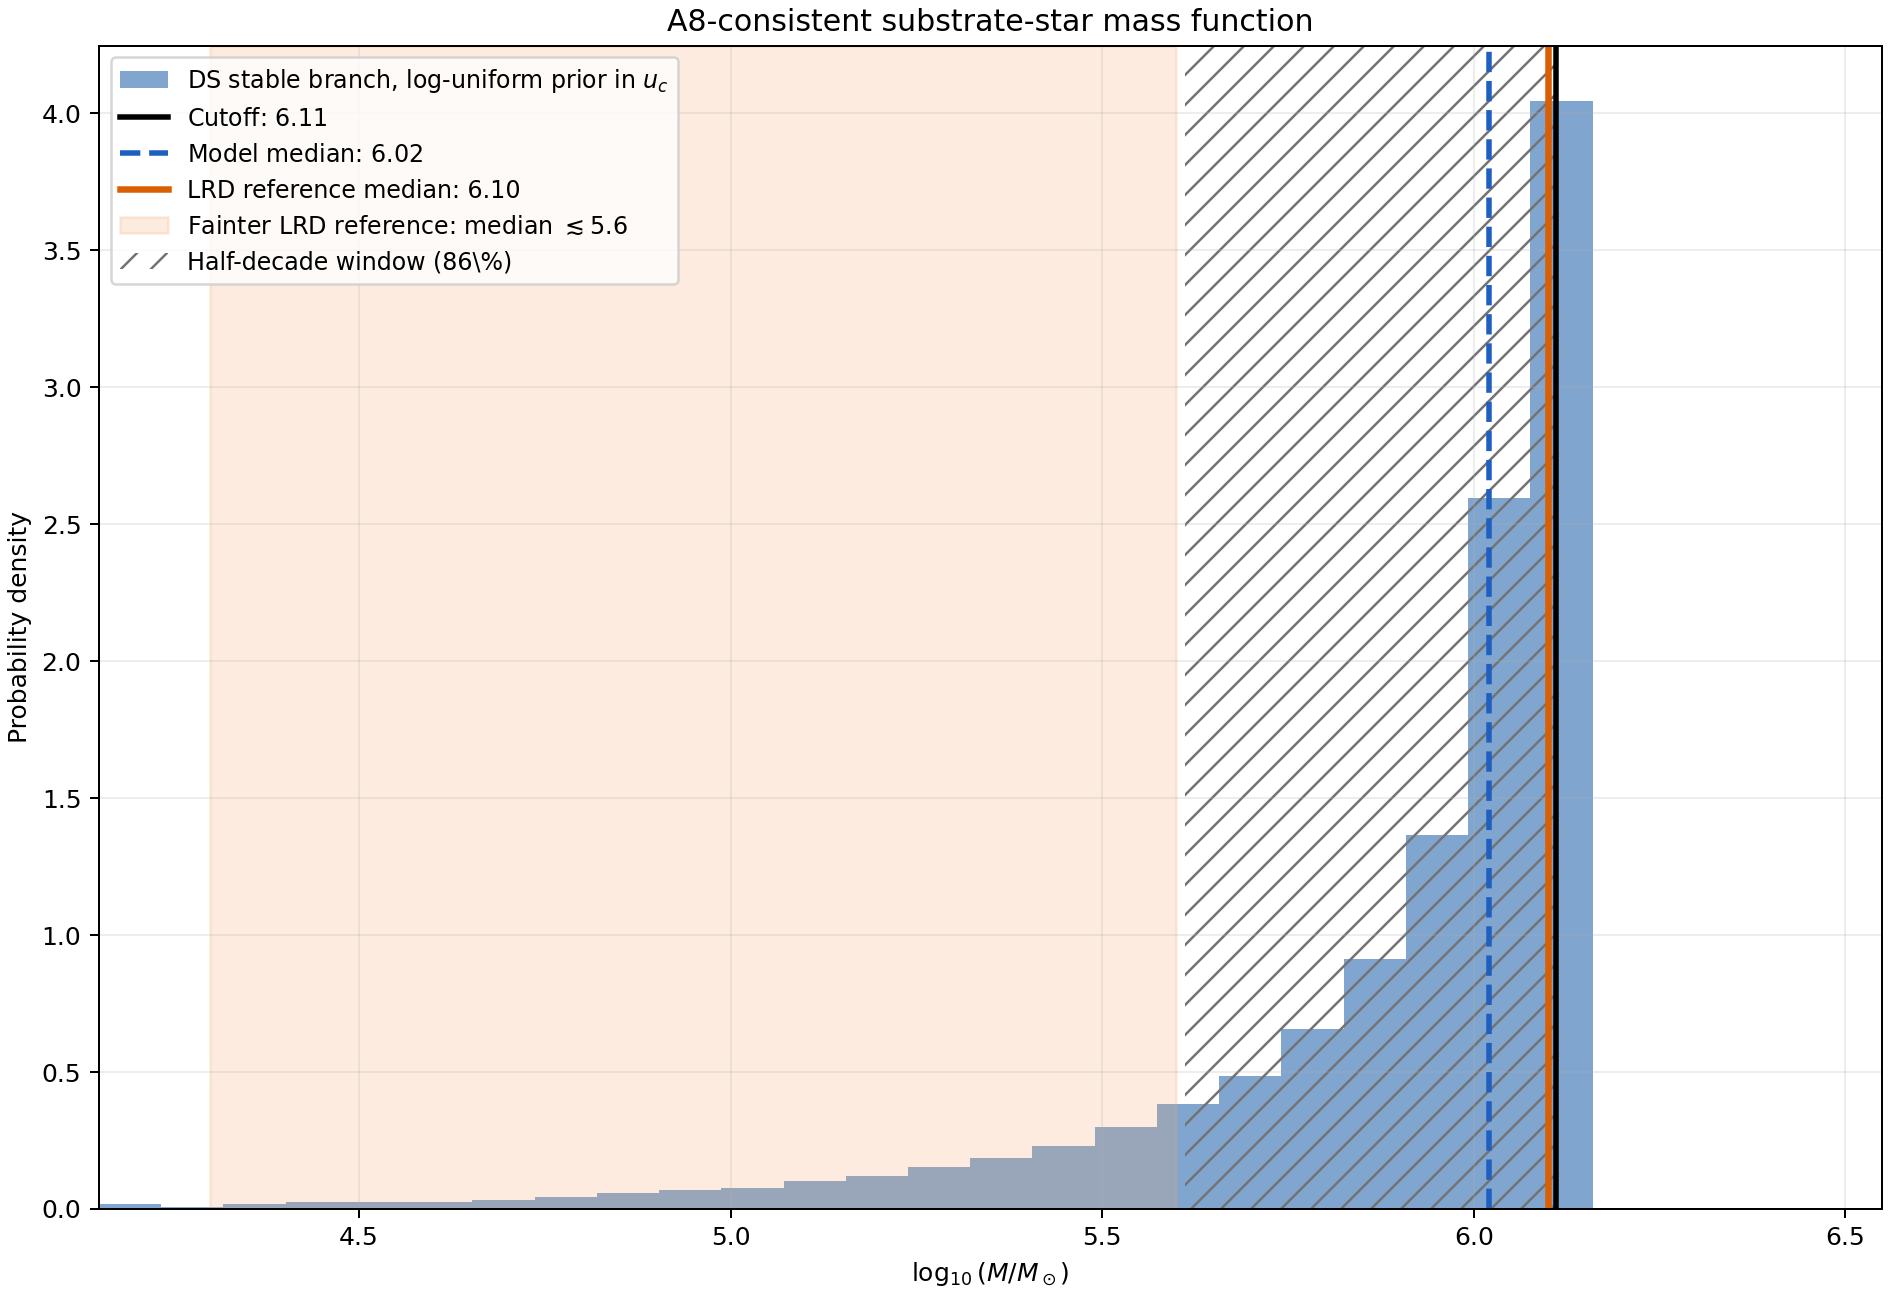
\includegraphics[width=0.82\textwidth]{fig_lrd.png}
\caption{Predicted substrate-star mass function (stable branch of Fig.~\ref{fig:branch} under a log-uniform prior in central density; blue histogram), regenerated from the A8-consistent dimensionless equations, with reference values from the electron-scattering-corrected Little Red Dot masses of Rusakov et al.\ \cite{rusakov2026}. The predicted median ($\log M = 6.02$) lies near the reported median of the seven firm masses ($\log M = 6.10$; orange line); the band indicates the 18 fainter objects (reported median $\log M \lesssim 5.6$), compatible with the low end of the branch (10\,\% quantile at $\log M = 5.49$). The hatched window is the registered prediction: a pile-up ($86\,\%$ on the corrected branch, $\sim80\,\%$ at deposit time) in the half-decade below the cutoff $\log M_{\text{crit}} = 6.11$. The independent dynamical-mass tension is discussed in the text and is not represented as a histogram datum.}
\label{fig:lrd}
\end{figure}

\paragraph{Analytic origin and prior-robustness of the accumulation.} The accumulation fraction is a caustic effect of the branch geometry, not a numerical accident: since $dM/du_c \to 0$ at the critical point, any smooth prior on the formation parameter $u_c$ piles objects up near $M_{\text{crit}}$ under the mapping $u_c \mapsto M(u_c)$. Analytically, for a log-uniform prior on $u_c \in [u_{\min}, u_{\text{crit}}]$, the fraction in the half-decade below the cutoff is
\begin{equation}
f_{1/2} = \frac{\ln(u_{\text{crit}}/u_*)}{\ln(u_{\text{crit}}/u_{\min})} \simeq 0.86 \quad (u_{\text{crit}}/u_0 = 14.5,\ u_{\min}/u_0 = 1.01,\ \text{corrected branch}),
\end{equation}
where $u_*$ is the central density at which $M = M_{\text{crit}}/\sqrt{10}$. Sensitivity to the prior (verified numerically on the corrected branch): $f_{1/2} = 86\%$ (log-uniform in $u_c$), $97\%$ (flat in $u_c$), $69\%$ (flat in $M$). The accumulation is thus robust, at the level $f_{1/2} \gtrsim 70\%$, for any smooth prior on the \emph{physical formation parameter}. It is erased ($f_{1/2} = 17\%$) only under a prior imposed flat on the \emph{observable} $\log M$ itself --- a choice that cancels the Jacobian by construction and corresponds to no formation channel populating central densities smoothly. The registered figure of $\sim80\%$ refers to the log-uniform baseline stated at deposit time (on the superseded branch; the corrected branch gives $86\%$); the robust, prior-independent statement is the existence of a pile-up with $f_{1/2} \gtrsim 70\%$ followed by a cutoff. Equivalently, and in the form least sensitive to recalibration: the differential mass function acquires an inverse-square-root divergence, $dN/dM \propto (M_{\rm crit}-M)^{-1/2}$, immediately below the cutoff --- the van~Hove exponent of a simple turning point, which is invariant under any smooth monotonic remapping of the mass scale.

\paragraph{Chandra X-ray constraint.} An independent line of evidence bears on the mass-calibration arbitration on which this test is conditional. Sacchi \& Bogd\'an \cite{sacchi2025} stacked $\approx400$~Ms of Chandra exposure on 55 LRDs and obtained a robust non-detection in the 0.3--7~keV band, ruling out unobscured super-Eddington accretion models unless obscuration is extreme ($N_H \gtrsim 10^{25}$~cm$^{-2}$, disfavored by JWST spectroscopy); they conclude that the black holes in LRDs are likely \emph{neither as massive nor as luminous} as the virial estimates suggested. This conclusion independently supports the low-mass calibration school (electron-scattering-corrected masses) on which the present confrontation is based, and disfavors the high-mass virial school under which Family~2 would be excluded. The X-ray quietness itself is not in tension with the substrate-star interpretation --- the model requires no super-Eddington accretion episode to reach the observed masses, since $M_{\text{crit}}$ is a structural scale rather than a growth endpoint; a quantitative accretion-luminosity model for substrate-star surfaces remains future work.

\paragraph{Registered prediction.} In the electron-scattering-corrected masses, the model predicts an accumulation of $\gtrsim 70\,\%$ ($86\,\%$ on the corrected branch, $80\,\%$ registered) of Family-2 objects in the half-decade below $M_{\text{crit}}$ ($5.6 \lesssim \log M \leq 6.11$) followed by a cutoff, whereas direct-collapse heavy-seed scenarios \cite{jeon2026} predict no preferred scale --- a discriminant accessible to the forthcoming JWST spectroscopic samples. This prediction is time-stamped by the v1.0 Zenodo deposit (version DOI: \href{https://doi.org/10.5281/zenodo.21196099}{10.5281/zenodo.21196099}), which predates the relevant future JWST data releases. The statistical criteria of the test are stated above (accumulation fraction, mass window, cutoff, and the $-1/2$ caustic exponent); any future modification of these criteria will be documented as a new version under the concept DOI (\href{https://doi.org/10.5281/zenodo.21196098}{10.5281/zenodo.21196098}), while the frozen record of the present prediction is the v1.0 version DOI above.

\paragraph{Experiments to watch}
Several ongoing experimental programs offer a direct validation window for the present model, without requiring a dedicated installation. (i)~The BIREF@HIBEF collaboration (European XFEL) is preparing a vacuum-birefringence measurement by a pump--probe scheme --- Petawatt laser as pump, X-ray beam as probe --- structurally analogous to the protocol proposed above; the proof of principle of dark-field detection, validating background suppression at the required level, was published in 2025~\cite{BIREF2025, Smid2025}. Any excess nonlinear vacuum response beyond the Euler--Heisenberg prediction would constitute a signature compatible with a population of stimulated micro-loops. (ii)~The VEGA gamma system at ELI-NP, continuously tunable from 1 to 19.5~MeV with a relative bandwidth below 0.5\,\%, will eventually permit an energy scan around the predicted cell resonance $E_1 = h c_0/\ell_1 \approx 1.53$~MeV. We correct here an earlier misstatement of this prediction: the Standard-Model $\gamma\gamma \to \gamma\gamma$ cross section is \emph{not} featureless in this window --- it is at its global maximum there ($\approx 1.61~\mu$b at $\sqrt{s} \approx 1.56$~MeV, dominated by the electron loop above the $2m_e$ threshold). The DS signature is therefore a \emph{narrow structure superposed on a QED background at its peak}, to be discriminated by lineshape rather than by excess alone; experimental sensitivity is also maximal there, which works in the measurement's favour. (Units: the 1.56~MeV figure is a two-photon $\sqrt{s}$, whereas $E_1 = 1.53$~MeV is a single-photon energy; the two coincide in order of magnitude but are not the same quantity.) (iii)~The ATLAS measurement of light-by-light scattering in ultraperipheral Pb--Pb collisions shows a residual tension of $\sim$1.8$\sigma$ with the best available theory after full NLO corrections~\cite{LbLNLO}. We downgrade this item to a \emph{watch}: the CMS measurement agrees with the same prediction, so the tension is ATLAS-only, and a genuine physical excess should appear in both experiments. The channel remains worth following, but it is not at present evidence for excitable micro-loops. (iv)~Finally, the PVLAS bounds on vacuum magnetic birefringence~\cite{PVLAS2020}, and their planned refinement by long-cavity interferometry on the ALPS~II magnet string (DESY)~\cite{ALPSII_VMB}, constitute the upper calibration constraints that the model's coupling coefficient $\delta Z/Z$ must respect in the static field.

\subsection{Newton's constant as topological closure: an exploratory conjecture}
\label{sec:g_closure}
The obstruction inventoried in Section~\ref{sec:open_problems} (item on the derivation of $G$) established that the conformal substrate ($P = u/3$) possesses no intrinsic scale and cannot by itself fix a dimensionless number of order $3/4\alpha$. The empirical identity retained there admits a suggestive rewriting. This subsection separates the part that can be obtained from transmission-line phase kinematics from the two additional bridges required for a derivation of Newton's constant.

With $R_3 = \hbar/m_e c_0$ (the unique calibrated length of the model: the loop circumference equals one Compton wavelength, $2\pi R_3 = \lambda_C$) and $\ell_1 = 2\pi R_3/3$, the identity $c_0^3\ell_1^2/2\pi\hbar \equiv hc_0/9m_e^2$ holds exactly, and the conjecture reads
\begin{equation}
G \;\stackrel{?}{=}\; \frac{c_0^3\,\ell_1^2}{2\pi\hbar}\,
\exp\!\left(-\,\frac{n}{4}\cdot\frac{\pi\varepsilon_0\hbar c_0}{e^2}\cdot 4\right)
= \frac{c_0^3\,\ell_1^2}{2\pi\hbar}\, e^{-n/4\alpha},
\qquad n = 3.
\label{eq:g_closure}
\end{equation}
\paragraph{Conditional phase-field normalization.} Let $\Phi$ be the circuit flux of one lossless string, with per-unit-length parameters $L'$ and $C'$. Its telegrapher action is
\begin{equation}
S=\frac12\int dt\,dx\left[C'(\partial_t\Phi)^2-\frac{1}{L'}(\partial_x\Phi)^2\right].
\end{equation}
After Wick rotation and the rescaling $y=c_0\tau$, using $c_0=1/\sqrt{L'C'}$ and $Z_s=\sqrt{L'/C'}$, the Euclidean action becomes isotropic. If, in addition, the phase is the compact canonical variable $\theta=q\Phi/\hbar$, then
\begin{equation}
\frac{S_E}{\hbar}=\frac{\hbar}{2q^2Z_s}\int d^2x\,(\nabla\theta)^2.
\label{eq:phase_action}
\end{equation}
Equation~\eqref{eq:phase_action} is a derivation from the telegrapher action \emph{conditional} on the canonical identification and compactness of $\theta$. Charge quantization in Axiom~A3 motivates but does not yet derive that identification from a microscopic Hamiltonian.

For a two-dimensional phase slip of winding $\nu$, $\theta=\nu\varphi$ outside a core of radius $a$, Eq.~\eqref{eq:phase_action} gives
\begin{equation}
\frac{S_{\rm slip}}{\hbar}=\frac{\pi\hbar\nu^2}{q^2Z_s}\ln\!\frac{L}{a}+\frac{S_{\rm core}}{\hbar}.
\label{eq:phase_slip_action}
\end{equation}
Under the simultaneous assumptions $q=e/3$, $Z_s=Z_0$, and a fractional winding $\nu=1/3$ on each of three equivalent strings, the logarithmic coefficient sums to
\begin{equation}
\Delta_{Z_3}=3\frac{\pi\hbar}{e^2Z_0}=\frac{3}{4\alpha}.
\label{eq:z3_coefficient}
\end{equation}
This is the precise result reached by the $Z_3$ route: a conditional coefficient of a logarithmic phase-slip action, not a complete instanton action. The fractional boundary condition is itself non-trivial. Standard finite-energy composite vortices in a three-component condensate have equal \emph{integer} windings; $(1/3,1/3,1/3)$ requires an explicit cyclic monodromy or string permutation after one turn. Neither that monodromy nor the microscopic phase-locking potential is presently derived in the DS model.

\paragraph{Why electromagnetic screening does not yet close the calculation.} A genuine charged condensate can screen the collective phase mode by the Anderson--Higgs mechanism, cutting the logarithm at a London length. The present telegrapher model, however, contains no independently defined charged order parameter, condensate density, kinetic inductance, London penetration length $\lambda_L$, or coherence length $\xi$. Its geometrical line inductance is not automatically a kinetic inductance, and the circuit flux $\Phi$ is not automatically a Higgs field. Hence neither $L/a$ nor $S_{\rm core}$ in Eq.~\eqref{eq:phase_slip_action} is fixed. The earlier identification of a unit logarithm with a cell choice, and the proposed automatic Anderson--Higgs cutoff, are withdrawn.

\paragraph{The two missing bridges to $G$.} Even if a microscopic calculation fixed $S_{\rm slip}/\hbar$ near $3/4\alpha$, a second equation would still be required to relate Newton's constant to a phase-slip fugacity or tunnelling amplitude. No such relation follows from the present gravitational field equations. Equation~\eqref{eq:g_closure} therefore combines (i) an empirical dimensionful prefactor, (ii) a conditionally motivated exponential coefficient, and (iii) an unproved identification of that exponential with gravitational coupling. It remains a conjecture, not a derivation.

\begin{table}[h]
\centering
\caption{Numerical sensitivity of Eq.~\eqref{eq:g_closure} to the trial coefficient $n/4$. Each increment of $n$ shifts $G$ by $e^{1/4\alpha} \approx 10^{15}$. The selectivity of the numerical match is not a derivation of the $Z_3$ boundary condition, the core action, or the coupling to gravity.}
\begin{tabular}{cccc}
\toprule
$n$ & $n/4$ & exponent $n/4\alpha$ & $G(n)/G_{\rm obs}$ \\
\midrule
1 & $1/4$ & $34.259$ & $5.3\times10^{29}$ \\
2 & $1/2$ & $68.518$ & $7.0\times10^{14}$ \\
\textbf{3} & $\mathbf{3/4}$ & $\mathbf{102.777}$ & $\mathbf{0.922}$ \\
4 & $1$ & $137.036$ & $1.2\times10^{-15}$ \\
\bottomrule
\end{tabular}
\label{tab:g_sensitivity}
\end{table}

Numerically (CODATA 2018): $c_0^3\ell_1^2/2\pi\hbar = 2.6598\times10^{34}$, $1/4\alpha = 34.259$, giving $G_{\rm pred} = 6.1570\times10^{-11}$ against $G_{\rm obs} = 6.6743\times10^{-11}$ --- a deficit of $-7.75\,\%$. The equivalent square-root forms halve the discrepancy: $\ell_P/\ell_1 = (1/\sqrt{2\pi})\,e^{-3/8\alpha}$ and $m_e/m_{\rm Planck} = (\sqrt{2\pi}/3)\,e^{-3/8\alpha}$, each accurate to $-4.0\,\%$.

\paragraph{The residual as the stated fact.} The coefficient that would reproduce $G$ exactly is $k = 0.74941135(16)$, i.e.\ $0.0785\,\%$ below $3/4$. This residual is \emph{not} measurement noise: it represents $\sim 3.5\times10^{3}$ standard deviations of the CODATA uncertainty on $G$, and two orders of magnitude beyond the inter-laboratory dispersion. Within a $\pm10\,\%$ window around $k$, the only simple fraction is $3/4$; but the conjecture stands or falls on deriving the $0.0785\,\%$ from the substrate, and no such derivation exists. Any mechanism invoked must produce this correction \emph{quantitatively}; qualitative appeals to sub-structure are pre-registered here as insufficient. We also pre-register the converse discipline: a numerical search over combinations of the model's constants will always produce a candidate matching a given residual to within a percent or so, and no such coincidence will be admitted unless the quantity is derived from a calculation and appears in at least one other, independent place in the framework.

\paragraph{Constraint and associated prediction.} The relation requires $\alpha$ at the Thomson limit --- consistent with $\alpha = e^2 Z_0/2h$, static by construction in this framework; using the running $\alpha(m_Z)$ misses $G$ by a factor $\sim 840$. Conversely, Eq.~\eqref{eq:g_closure} implies $\Delta G/G = (3/4\alpha)\,\Delta\alpha/\alpha \approx 103\,\Delta\alpha/\alpha$: existing bounds $|\Delta\alpha/\alpha| < 10^{-5}$ then impose $|\Delta G/G| < 10^{-3}$, an order of magnitude tighter than the direct lunar-laser-ranging constraint --- a universal drift with epoch, never a species-dependent one.

\paragraph{Status.} Equation~\eqref{eq:phase_action} is a conditional derivation from transmission-line kinematics. Equation~\eqref{eq:z3_coefficient} is a conditional scaling result requiring compact fractional monodromy and $Z_s=Z_0$. Equation~\eqref{eq:g_closure} is an exploratory conjecture. The scale ratio, core contribution, $Z_3$ monodromy, charged-order-parameter sector, and the mapping from instanton fugacity to $G$ remain open; the numerical residual must not be treated as a radiative correction until one is calculated from a specified action.

\section{Open Problems and Limitations}
\label{sec:open_problems}
For transparency toward the reader, the following inventory lists the model's principal open problems, in decreasing order of severity. None of these is glossed over elsewhere in the document; this section gathers them.

\begin{enumerate}
    \item \textbf{Neutrino sector (major).} Three readings all fail against table data: massless unfolded states are excluded by oscillations ($\Delta m^2_{21} = 7.5\times10^{-5}$~eV$^2$, $|\Delta m^2_{31}| = 2.5\times10^{-3}$~eV$^2$); the inductive micro-loop mass $L/\kappa \approx 0.12$--$0.58$~MeV overshoots $\Sigma m_\nu < 0.12$~eV by $\ge 10^{6}$; the WKB-weighted effective mass ($p \approx 1.4\times10^{-4}$) $\approx 40$~eV still overshoots by $\sim$300. One $\Ncd=2$ topology cannot host three flavors ($N_\nu = 2.984 \pm 0.008$, LEP) nor PMNS mixing. A candidate direction --- the DQD opening amplitude as the flavor coordinate --- is recorded as Postulated, requiring (i)~quantization to exactly three levels, (ii)~an opening$\to$mass law reproducing the $\Delta m^2$ ratio $\approx 33$, (iii)~a mixing mechanism. We add a structural remark that sharpens the difficulty: the mechanism favoured in the Standard-Model literature makes neutrino masses small by being \emph{inversely} proportional to a large scale, whereas every mechanism available in the present framework makes them \emph{directly} proportional to the available scale. The mismatch is one of sign in the exponent, not of magnitude, and no inversion mechanism is available here.
    \item \textbf{Microscopic derivation of the medium.} The DQD gas and its bifilar transmission-line representation are postulated, not derived from a microscopic Hamiltonian or partition function. Until the distributed RLC parameters are shown to emerge from a well-defined statistical mechanics of DQDs, the model remains, in the apt phrase of the AI-based critical evaluation, a structured set of analogies rather than a physical theory. This is the deepest debt.
    \item \textbf{Quantum interpretation and decoherence.} The low-impedance corridor and its no-signaling narrative have been withdrawn (Section~\ref{sec:nonlocal_correlations}). The model currently has no state-space construction for entangled defects, no Born rule, no measurement map, and no decoherence functional. A viable quantum extension must reproduce Bell correlations without an operational signaling channel and must derive the reduced-state dynamics of a subsystem from a specified microscopic action. These are constraints to be met, not phenomena presently explained by the DS model.
    \item \textbf{Quantitative quantum sector.} The hydrogen spectrum recovery (Section~\ref{sec:kinematic_gravity}) is structural ($E \propto -1/(n^*)^2$), not quantitative: the Rydberg constant is not yet derived from substrate parameters. Appendix~\ref{app:schrodinger} now supplies a partial answer on the \emph{kinematic} side: on the surrogate Johns lattice, the envelope of a localized excitation obeys the free Schr\"odinger equation as its single-band quadratic truncation, a single action quantum closes both the de~Broglie relations and the inertial response, and an external potential enters exactly as in solid-state envelope theory, with a measured breakdown threshold. What remains interpretive is the \emph{dynamical} side, and it is the harder half: a self-consistent potential generated by a second defect (hence the hydrogen problem itself), the Born rule, and the measurement process. Two negative results delimit the gap: the bound-band coupling between two braided defects falls off exponentially with separation, so the $1/r$ potential cannot originate there and must come from the charge sector; and the exact stationary states of the bare lattice carrying a point charge are anisotropic, the isotropic Coulomb field being recovered only in the continuum limit, with violation measured to fall off as $\approx 1.4\,\ell_1/r$.
    \item \textbf{Strong-field and radiative gravitational sector.} With the scalar sector constrained and the tensor sector bootstrapped to GR, the exterior is Schwarzschild and no deviation is predicted; the burden has moved entirely to the tensor sector, whose bootstrap is asserted (Deser) rather than performed: the quadrupole formula, the polarization content and the GW luminosity all await that computation (Section~\ref{sec:tensor_sector}). \emph{Interior--exterior matching (new).} The interior of Section~\ref{sec:substrate_stars} is integrated with the scalar force law, while the exterior is Schwarzschild; at the surface of the critical configuration $U = GM/Rc_0^2 \approx 0.4$, so the two descriptions differ there at second post-Newtonian order by $O(1)$ coefficients. A matched interior--exterior solution has not been constructed, and the numbers of Section~\ref{sec:substrate_stars} (Newtonian interior) are exposed to this uncertainty in addition to those already listed.
    \item \textbf{Preferred-frame parameters not computed.} The scalar action contains no explicit substrate 4-velocity, but the effective metric singles out a time direction through the field itself, and the boosted profile solves the field equation only to first order (Sections~\ref{sec:kinematic_gravity},~\ref{sec:lorentz}). Establishing or excluding $\alpha_1 = \alpha_2 = 0$ requires a post-Newtonian computation performed with the substrate frame in motion relative to the system, which has not been done. Until then the model's standing against the Einstein-aether bounds is undetermined rather than clear.
    \item \textbf{Aspect ratio $R_3/r$ and the loop phase.} Two dimensionless inputs of the particle sector are undetermined: the aspect ratio $R_3/r \approx 37.1$, on which $Z_e$ depends logarithmically (Section~\ref{sec:electron_impedance}); and the accumulated interface phase $\theta_{\text{tot}}$ of the single-valuedness condition~\eqref{eq:single_valued}, which fixes the offset of the radial mode ladder. Neither follows from the matching condition, which constrains $D/r$ only.
    \item \textbf{Derivation of $\ell_{\text{cell}}$.} The local cell spacing is a cosmological initial condition postulated equal to $\ell_1$ at rest; $\Pi_{\text{sat}}$, $\omega_c$, and the saturation coefficient are conditional on it.
    \item \textbf{Newtonian interior treatment.} The hydrostatic integration of Section~\ref{sec:substrate_stars} treats momentum non-relativistically at compactness $\sim0.8$; a covariant reformulation could shift $M_{\text{crit}}$. The second implementation has been re-run on the A8-consistent source; the first has not, and the two-implementation agreement stated in earlier versions refers to the superseded source.
    \item \textbf{Two-component interior of accreting substrate stars.} The interior of Section~\ref{sec:substrate_stars} contains substrate only. An accreting Family-2 object also contains ordinary matter, and because the equilibrium substrate is transparent ($\Gamma_{\text{bif}} = 0$) it exerts no pressure on that matter, which falls to the centre and forms a separate compact core inside the substrate halo (Section~\ref{sec:lrd}); the density scales of the two components differ by $\gtrsim 10^{9}$ and never meet. Three consequences are open. (i)~The core gravitates through the same field $Z$ and modifies the substrate profile from the inside; whether the stable branch and $M_{\text{crit}}$ survive a central point-like mass of fraction $f$ is a two-component hydrostatic calculation that has not been done, and its answer sets the maximum matter content compatible with the branch. (ii)~The photosphere of an accreting object sits at the core, not at $R$, so the thermal-surface signature is at present a luminosity constraint only; its spectral form (temperature, extent) requires (i). (iii)~Because the substrate is diffuse (mean density of white-dwarf order at $M_{\text{crit}}$) while its gravitational compactness reaches $r_s/R = 0.81$, no unification of matter and substrate at the stellar level is possible in this framework: the compact object is a diffuse state of the vacuum, not compressed matter. This item follows directly from the transparency axiom, the most solid of the model, and is retained until the calculation exists.
    \item \textbf{Statistical power of the LRD test.} The present sample ($n=7$ firm masses) cannot discriminate; the registered prediction (Section~\ref{sec:lrd}) is the operative test.
    \item \textbf{Formalization of the distributed phase-lock.} The phase-locking (PLL) mechanism invoked to confer coherence on the substrate --- lattice rigidity (Section~\ref{sec:conceptual}), the transparency clause $\chi_{\text{vac}}\ll1$ (Section~\ref{sec:atomic_repulsion}), and the nematic order underlying A7 (Section~\ref{sec:tensor_sector}) --- is at present a name imported from electronics, without governing equations. It is no longer invoked as an entanglement mechanism. The natural formalization is a distributed injection-locking / Kuramoto dynamics on the DQD gas, with the coupling supplied by the pole reflections $\Gamma_{\text{pole}}$ and the whole read as axiom A4 (relaxation toward $|\Gamma|^2$ minimum) in servomechanism form; deriving the phase stiffness $\rho_\phi$ from this dynamics --- and with it $\langle\delta Z^2\rangle$, $\chi_{\text{vac}}$, and the shear modulus in one stroke --- is a stated target. The difficulty is now quantified. Three attempts to compute $\chi_{\text{vac}}$ at the level of a single cell all failed, and failed differently: a gradient--quadrupole coupling (invalidated by a confusion between the cancelled magnetic moment and the uncancelled electric dipole of the cell); a wall-stiffness calculation displacing $D$ about $D_0$ under field (illegitimate, since A5 forbids continuous deformation; it gave $\chi_{\text{vac}} \sim 2\times10^{-4}$, eighteen orders above the PVLAS bound); and a Kuramoto-torque calculation respecting A5 (twelve orders above the bound). Estimates disagreeing among themselves by six orders of magnitude exclude a merely wrong constant and indicate that no single-cell picture can supply the observed protection: the suppression must be collective. The natural candidate, the Bohr--van Leeuwen cancellation of a classical equilibrium gas, is real but fixes the \emph{total} moment of a bounded system through boundary currents, not the \emph{local} response probed by a laser beam far from any wall. The correctly posed residual question is therefore whether the ordered DQD gas has a finite statistical coherence length $\xi$ inside which such a cancellation reconstitutes itself, and whether $\xi$ is small against laboratory beam scales; no value for $\xi$ exists anywhere in the model. The scale-dependent discriminant of Section~\ref{sec:discussion} is the testable residue of this open problem.
    \item \textbf{Status of the weave chirality (resolved, with a residual question).} The chiral closure formerly listed here is \emph{dissolved}: the Johns matrix is invariant under the full point inversion and under every mirror ($O_h$), so the scattering never receives the weave handedness as an input, and the $\pm\tfrac12$ signs originate in the achiral vector-product algebra of constraint C3 (Section~\ref{maxwell3d:chirality}). Theorem~4 carries no residual chiral postulate. What remains open is the converse question: the geometric chirality of the weave is real but \emph{mute} in the electromagnetic sector, and no mechanism is given by which it could acquire physical relevance where parity is not protected. The muteness is confirmed on two independent fronts --- the achirality of the scattering matrix, and the electrostatics of a charged braided defect, for which the two mirror weaves are found degenerate. A chiral constitutive term of the Dzyaloshinskii--Moriya type would be the natural carrier, and it would simultaneously evade Derrick's theorem: for an energy functional $E(\lambda) = A\lambda^3 + B\lambda^2 + C\lambda$ in three dimensions (potential, one-derivative chiral term, gradient), a finite equilibrium size exists if and only if $|B| \geq \sqrt{3AC}$, whereas without the chiral term the energy is monotonic and the localized configuration collapses. Stabilizing an object at the Compton scale in this way would require a vacuum chirality of order unity at that scale, which is excluded by bounds on the rotation of astrophysical polarization by more than thirty orders of magnitude. \emph{The muteness of the weave and the absence of stable three-dimensional solitons in this framework are therefore one constraint, not two.}
    \item \textbf{Derivation of $G$ --- conditional progress, obstruction retained.} The telegrapher action fixes the compact-phase normalization conditionally, and three strings with $q=e/3$, $Z_s=Z_0$, and fractional winding $1/3$ yield the logarithmic coefficient $3/4\alpha$ (Section~\ref{sec:g_closure}). This does not fix the logarithm, the core action, or even the required fractional monodromy. More decisively, no equation relates the resulting phase-slip fugacity to the gravitational coupling. The conformal obstruction therefore remains: an independently derived scale and a microscopic coupling to the gravitational sector are both missing. The identity $G = 1.084\,(hc_0/9m_e^2)\,e^{-3/4\alpha}$ is retained as an unexplained numerical fact, and the $0.0785\,\%$ residual in its fitted exponent is a target rather than evidence of a calculated correction.
    \item \textbf{Absence of a mass scale --- the obstruction stated in general form.} The preceding item concerns $G$; the same obstruction governs every mass in the framework, and it is worth stating once in its general form because it delimits what this model can and cannot aim at. A vacuum that is purely electromagnetic and impedance-matched is conformally invariant and therefore possesses no intrinsic scale. Four independent analyses converge on this conclusion: the equation of state $P = u/3$; the single-velocity character of the linear lattice; the zero-point sum over the braided defect, which is a pure ultraviolet term proportional to the cutoff; and, at the non-linear level, the fact that the soliton-to-quantum mass ratio of a transmission line is fixed by its characteristic impedance alone. The last of these deserves emphasis, because it is the only one that is not blind to non-perturbative structure: for a line of impedance $Z$, the relevant dimensionless coupling is $Z e^2/2\hbar$, so matching of the substrate ($Z = Z_0$) gives $2\pi\alpha$, and \emph{any} soliton of that line --- irrespective of the non-linear constitutive relation assumed --- weighs $O(1/\alpha)$ times its own quantum. Strong coupling would require $Z \approx 174\,Z_0$, incompatible with the transparency of the vacuum. The consequence is stated plainly: $m_e$ is not ``not yet derived'' in this framework, it is structurally an \emph{input}, exactly as the corresponding Yukawa coupling is an input of the Standard Model; and the electron is to be read as the \emph{quantum} of the line rather than as its soliton. What remains attainable is a spectrum of \emph{ratios} given one scale, not an absolute mass. A related caution is recorded: the characteristic impedance of a \emph{line} ($\sqrt{L/C}$ of a conductor geometry) and the impedance of the \emph{medium} ($\sqrt{\mu/\varepsilon}$, which sets $\alpha = e^2 Z_0/2h$) are distinct quantities; raising the former by coiling does not raise the coupling, so no confinement-type strong-coupling regime can be reached by winding a line, only by changing the medium itself.
    \item \textbf{Charge as chirality: pair creation and the P--C identification.} With charge carried by winding chirality, three structural consequences follow. (i) The vacuum node being achiral (Theorem~4, $O_h$-invariant scattering), net chirality is conserved and equal to zero; chiral solitons can therefore only be created in mirror pairs. Charge conservation, already verified at the node level (constraint C2), thereby acquires a second, topological root. (ii) Annihilation becomes mechanical: two mirror windings meeting untwist into the achiral vacuum, releasing their energy as achiral $\Ncd = 1$ solitons. (iii) Spatial inversion exchanges the two winding senses (Section~\ref{maxwell3d:chirality}: $-\mathbb{1}$ maps the two weaves onto each other); parity therefore \emph{acts as} charge conjugation --- the mirror image of an electron is a positron. This identification is invisible to the emergent electromagnetic sector, which respects P and C separately; any contact with the weak sector, where P and C are separately violated, lies outside the model's scope. A further limitation is recorded here: the charge itself is not carried by the connectivity of the linear network. A stationary state bearing a net flux through a closed surface requires a genuine divergence source within it, and the braided defect --- with either handedness, and at equal cost --- provides none. If charge exists in this framework it must reside in the constitutive content of the string (the $e/3$ energy fluid of Section~\ref{sec:conceptual}), whose equation of state is unspecified. The declared debt of the construction is cosmological: strict pair creation implies exact matter--antimatter symmetry at formation, making the observed baryon asymmetry an open problem of the framework, as it is of the Standard Model.

    \item \textbf{Genesis conjecture (unconstrained).} The primitive state is conjectured to be the defect-free cubic lattice of Section~\ref{sec:bifilar_model}; a quench during its condensation (Kibble--Zurek mechanism) would freeze in chiral loop defects by pairwise string reconnection --- a mechanism that produces closed, chiral loops with a minimum circumference $\sim \ell_1$, consistent with a discrete stable spectrum. Neither the quench nor the reconnection dynamics is derived; the entry records a research direction, not a result. The behaviour of a fixed-$\ell_1$ lattice under cosmological expansion is a second open question of the same sector.

    \item \textbf{Proton characteristic impedance --- open derivation.} The mass law $m \propto \Ncd^2 Z_{\Ncd}$ with $m_p/m_e = 1836$ and $N_p/N_e = 9$ requires $Z_p/Z_e \approx 22.7$ (the same factor already appearing as the current ratio $I_p = 22.7\,I_e$ in Section~\ref{sec:kinematic_gravity}). A closed toroidal-helix geometry for the $\Ncd = 27$ soliton (9 turns of 3 strings, mutual inductance $L \propto N^2$, series inter-turn capacitance $C \propto 1/N$) yields $Z_p/Z_e = N^{3/2} = 27$ --- within $19\,\%$ of the required value, a residual of logarithmic order comparable to the $\ln(8R_3/r)$ corrections of the electron derivation. Closing this gap from an internal matching condition, without fitting, would render the proton mass geometric; the derivation is open.
    \item \textbf{Rotation sector.} The model is static; real compact objects spin, and Blandford--Znajek jet launching requires an ergosphere. The vorticity field of the ansatz ($-Z_{\rm base}\beta^2_{\rm vtx}$, lowering local impedance) is the natural frame-dragging analogue; a ``Kerr analogue'' (frozen collapse + frozen vorticity) is an open construction. Jets themselves pose no conflict (launched outside the photon sphere).
    \item \textbf{Semiclassical formation flux.} The transient Hawking-like emission during collapse (BLSV class) requires curved-space QFT beyond the present framework.
\end{enumerate}

%============================
\section{General Conclusion}
The Dipolar Strings physics presented in this document is an exploratory, phenomenological model that approaches the nature of matter and vacuum through an analogical mechanics anchored in transmission-line electrodynamics. By imagining space as a capacitive and inductive (LC) physical substrate where point particles give way to simple topological nodes, new perspectives take shape.

This edition proposes the common physical level beneath General Relativity and Quantum Mechanics --- both held exact in their domains --- a single ontology underlying the two pillars at once. Beneath GR, the DS model \emph{extends}: where the singularity theorems mark the end of validity of the Einsteinian continuum, the substrate takes over and delivers finite equilibria --- a stable branch of substrate stars without horizon or singularity, endowed with a preferred mass scale $M_{\text{crit}} \propto \ell_1^2$ issued from the medium's constants alone, and frozen collapses everywhere else. Beneath QM, the DS model now \emph{partly derives} rather than merely interprets: on a surrogate lattice, the envelope equation, the action quantum, the de~Broglie relations and the inertial response follow from the medium without quantum input (Appendix~\ref{app:schrodinger}), while the self-consistent potential, the Born rule and the measurement process remain interpretive. The asymmetry of maturity between the two arms is assumed: quantitative on the gravity side, partial on the quantum side, and explicitly closed on the matter side, where the conformal obstruction (Section~\ref{sec:open_problems}) makes the electron mass an input rather than a derivable quantity.

\paragraph{Broader impact.} Beyond its specific claims, this program bears on three wider questions. For astrophysics, a confirmed preferred mass scale in the compact-object mass function would reshape the seeding problem of supermassive black holes, replacing growth histories with a structural attractor. For foundations, the model is a concrete test case of how far the analogue-gravity paradigm \cite{barcelo, volovik} can be pushed from laboratory analogy toward candidate ontology, and of what evidential standards such attempts must meet --- the fully AI-mediated revision trajectory of this document, preserved in Appendix~A, is offered as a methodological data point in itself. For scientific practice, the manuscript documents a fully disclosed human-AI collaboration protocol (falsification-partner mode, independent re-implementation, symbolic verification) that may be useful to other independent researchers; its limitations --- chiefly, that both numerical implementations originate from the same collaboration --- are stated rather than hidden. The speculative status of the model is reaffirmed: nothing in this document should be read as a validated contribution until the designated falsification targets have been confronted with data.

The path from coherent analogue model to validated physics passes through a quantitative prediction before the measurement. With a Schwarzschild exterior the model predicts nothing new outside compact objects; its content is in the limit states: the permanent absence of PBH evaporation bursts (binary), the geometrically spaced echoes of fresh merger remnants, and the mass function of intermediate-mass compact objects near $M_{\text{crit}}$ (JWST, then the LISA window). Until then, this working model constitutes an alternative modeling whose relation to General Relativity is intended to parallel the relation of molecular theory to continuum hydrodynamics: not a contradiction, but a candidate microstructure for a continuum theory that is exact in its domain.

\section*{Data Availability}
This manuscript, together with its supplementary files, is archived on Zenodo under the concept DOI \href{https://doi.org/10.5281/zenodo.21196098}{10.5281/zenodo.21196098} (which always resolves to the latest version); the v1.0 version DOI \href{https://doi.org/10.5281/zenodo.21196099}{10.5281/zenodo.21196099} serves as the time-stamped record of the registered prediction of Section~\ref{sec:lrd}. The supplementary files of the present version include: the two independent implementations of the hydrostatic equilibrium integration (Section~\ref{sec:substrate_stars}) and the equilibrium-sequence data; the figure-generation scripts (Figs.~\ref{fig:branch}, \ref{fig:lrd}, \ref{fig:heaviside}); the SymPy scripts for the symbolic verifications (the 1PN/2PN expansions of Section~\ref{sec:ppn}; Theorem~3, the conformal identity $g_{\text{iso}} = e^{\chi}g$, and the boosted-solution residual); the master script \texttt{p2\_master.py} reproducing all breather results of Appendix~\ref{app:breathers}, including the open-system control; and the scripts of Appendix~\ref{app:schrodinger} (\texttt{calc1.py}, \texttt{calc1b.py}, \texttt{calc3.py}, \texttt{calc2.py}, with the shared module \texttt{calc1\_common.py}). The package ships a frozen environment specification (\texttt{requirements.txt}) and the rerun log of the verification suite (40/40 PASS, exit 0, 2026-07-23); the manuscript and figures are released under CC BY 4.0, the code under the MIT licence. All numerical results are reproducible from the structure equations~\eqref{eq:star_structure}, which fully specify the integration.

\section*{Acknowledgments and Methodological Disclosure}
The development of this work was carried out in extensive collaboration with Claude (Anthropic), used as a computational assistant, critical falsification partner (``guard-rail''), and writing assistant, under the direction of the author. The founding physical intuition (the vacuum as an impedance-matched transmission-line network), the dipolar-string concept, and the transmission-line derivations of Sections~\ref{sec:bifilar_model}--\ref{sec:electron_impedance} originate with the author, an electrical engineer. The general-relativistic and field-theoretic formalization --- including Theorem~3, the conformal-representative analysis, the post-Newtonian expansions, the tensor-sector construction, the hydrostatic integrations and their re-implementation, the lattice computations of Appendix~\ref{app:schrodinger}, the statistical analyses, and the English text --- was generated primarily by the AI assistant in response to successive rounds of AI-based critical evaluation (SciSpace), and the author does not claim independent command of this layer. All research decisions and the decision to archive this document are the author's. The document is offered as an exploratory working hypothesis and a documented case study of AI-assisted independent research --- not as a validated contribution or a claim of expertise in general relativity or quantum field theory on the author's part. Both numerical implementations originate from this same collaboration; independent third-party verification has not yet been performed, and the reader is invited to reproduce the results from the structure equations~\eqref{eq:star_structure} and the released code.

All external critical evaluation of this manuscript was performed by an AI-based review tool (SciSpace, formerly Typeset), operating independently of the primary AI collaborator (Claude, Anthropic). \textbf{No human peer review has taken place at this stage.} The revision trajectory preserved in Appendix~A therefore documents an entirely AI-mediated revision process, disclosed here as part of the manuscript's fully declared human--AI collaboration protocol.

\newpage
\appendix

%==============================================================================
\section{Document History}
This article consolidates a sequence of working documents (V1.8 through V2.6, 2025--2026); V2.7 adds Appendix~\ref{app:breathers} (proof of mechanism for emergent relativistic dynamics, with measured second-order convergence) and its anchors in Section~\ref{sec:lorentz}. V2.8 adds Section~\ref{sec:g_closure} (Newton's constant as topological closure --- exploratory conjecture, sensitivity table, residual stated) and Appendix~\ref{app:schrodinger} (emergent single-band Schr\"odinger dynamics on the Johns lattice); it harmonizes the status of the weave chirality across Sections~\ref{maxwell3d:chirality}, \ref{sec:electrodynamic_synthesis} and~\ref{sec:open_problems} (the chiral closure is \emph{dissolved}, not residual, and is now tied to the absence of three-dimensional solitons), states the conformal obstruction in general form as a limitation on any mass derivation, restates Theorem~4 with its inputs made explicit, corrects the description of the QED $\gamma\gamma\to\gamma\gamma$ background near 1.5~MeV, downgrades the light-by-light item to a watch, adds the calibration-invariant $-1/2$ caustic exponent to the registered LRD prediction, and adds a terminological disambiguation in Section~\ref{sec:related_work}. The validated gravitational core is unchanged. V2.9 responds to an external critical review by repairing four points that touch load-bearing structure rather than presentation: the quantization condition of Section~\ref{sec:impedance_confinement} is rederived from single-valuedness on the closed loop, the earlier derivation from $|\Gamma| = 1$ being withdrawn as invalid; the field equation of the scalar sector is given explicitly and the claim that the Heaviside profile is an \emph{exact} boosted solution is downgraded to first order, with $\alpha_1 = \alpha_2 = 0$ correspondingly downgraded from result to open problem; the electron impedance $Z_e$ is reclassified as \emph{Calibrated}, the aspect ratio $R_3/r$ having no derivation, and the model's input count corrected from one to two; and the little-red-dot confrontation is demoted following a direct dynamical mass measurement favouring the high-mass calibration, with the horizon-signature analysis of GW250114 added to the observational pressures on the horizonless family. All four changes reduce the model's claims. The present revision of V2.9 (late August 2026) makes four further changes, three of which again reduce the model's claims: (a)~the statement that Family-2 substrate stars ``must display a thermal photosphere'' is withdrawn as unestablished --- the transparency of the substrate implies a two-component interior (compact matter core inside a diffuse substrate halo) whose hydrostatics has not been computed, so the thermal-surface signature is retained as a luminosity requirement only (Section~\ref{sec:lrd}, new open problem); (b)~three failed single-cell computations of $\chi_{\text{vac}}$ are recorded under the phase-lock open problem, together with the Bohr--van Leeuwen argument and its limits; (c)~a scale-dependent birefringence discriminant that does not require the coherence length is added in Section~\ref{sec:discussion}; (d)~an equivalence-principle consistency remark on the minimal-coupling clause is added in Section~\ref{sec:conformal_representative}, and the line-impedance/medium-impedance distinction is recorded under the mass-scale obstruction. A subsequent consistency audit (28 August 2026) repaired three internal contradictions, each of which reduces the model's claims: (e)~the scalar sector is declared constrained (elliptic) throughout, consistently with Section~\ref{sec:tensor_sector}; the propagating reading of Eq.~\eqref{eq:lagrangian} and its GW170817 prefactor argument are withdrawn, since a propagating scalar carrying the Newtonian coupling would radiate at order unity relative to GR (Hulse--Taylor) and would carry a breathing mode; (f)~Axiom~A8 is now implemented in the structure equations (source $u - u_0$), which lowers $M_{\text{crit}}$ from $1.62$ to $1.29\times10^{6}\,M_\odot$ and the maximal compactness from $1.22$ to $0.81$, so that stable substrate stars no longer lie inside their Schwarzschild radius; (g)~the Deser bootstrap is taken to its stated endpoint, the exterior of compact objects is Schwarzschild, and the shadow-diameter ($+4.63\,\%$), ISCO and 2PN deviations are withdrawn as properties of the scalar profile alone; the echo argument is rederived in Schwarzschild (geometric spacing) and the falsification hierarchy renumbered. Figures~\ref{fig:branch} and~\ref{fig:scaling} are regenerated on the corrected branch; Figure~\ref{fig:lrd} is flagged for regeneration. The sequence was developed through several rounds of AI-based critical evaluation (SciSpace; no human peer review has taken place). The complete version-by-version change log --- including all errata, closed research fronts (spin-2 from scalar/vector fields, the $w=-1$ cosmological sector, photon--electron scattering, near-horizon reflective surfaces) and the AI-mediated revision trajectory --- is archived with the versioned Zenodo record of this manuscript (concept DOI: \href{https://doi.org/10.5281/zenodo.21196098}{10.5281/zenodo.21196098}). The registered prediction of Section~\ref{sec:lrd} is time-stamped by the Zenodo deposit accompanying this article; its statistical criteria are frozen as stated in that record.

%==============================================================================
\paragraph{V2.9.1 Zenodo edition (31 August 2026).} This publication edition preserves the complete V2.9 manuscript and makes a further conservative quantum-sector audit. The low-impedance entanglement corridor, its synchronization-speed formula, Bell-derived bounds, and measurement-induced PLL-unlock narrative are withdrawn because no governing equation in the model supports them. Phase opposition is retained only as a conditional differential normal mode, not as a derived pair-creation or entanglement mechanism. In the $G$ conjecture, the telegrapher action is used to derive the compact-phase stiffness conditionally: with $q=e/3$, $Z_s=Z_0$, and three fractional windings $1/3$, its logarithmic coefficient is $3/4\alpha$. This is explicitly separated from a complete instanton action and from the still absent equation connecting instanton fugacity to Newton's constant. The required fractional monodromy, core and screening scales, charged order parameter, kinetic inductance, and London/coherence lengths are listed as missing rather than imported from a superconducting analogy. The superseded 29-page reduction is not part of this record; the present source is the complete manuscript with all appendices and figures.

%==============================================================================
\section{Fundamental Table of Elementary Particles}
%==============================================================================
The table below is a reverse-engineered parametrization, not a set of predictions; see the Scope statement of Section~1. In line with that statement --- the framework is a theory of the medium, not of matter --- this edition retains only the three states within scope: the photon ($\Ncd=1$ soliton), the DQD constituent of the vacuum ($\Ncd=2$), and the electron ($\Ncd=3$), the model's unique calibration anchor. The previously tabulated assignments for the muon, tau, and the weak bosons ($W$, $Z$, $H$) were reverse-engineered mass fits without predictive content and are withdrawn from the catalogue.

\begin{remarkstar}[Warning --- calibrated catalogue, not predictions]
The index assignments in this table are the result of phenomenological reverse engineering against the experimental masses, under the charge-quantization constraint. They are working hypotheses of the exploratory framework A1 --- \emph{none} of the entries below constitutes a prediction of the model, and the table must not be read as one. The model's predictive content resides in the derived quantities listed in the epistemological status classification (Section~\ref{sec:electrodynamic_synthesis}), not here.
\end{remarkstar}

\paragraph{Methodological note on the calibration of the indices}
For development purposes, we have elaborated a postulated $\Ncd$ index system, fully assumed as a working framework. In this formalization, it is posited that charge is dictated topologically by the \emph{winding chirality} of the closed loop --- the two mirror senses of circulation carrying opposite signs, with the magnitude $e/3$ per string fixed independently by the interface coefficient $\Gamma_{\text{pole}} = 1/3$ (Section~\ref{sec:bifilar_model}) --- and that mass follows from a closed-loop weight. All solitons of the catalogue are closed structures; no open terminations are invoked. This assignment addresses the question left open in Section~\ref{maxwell3d:chirality}: the geometric chirality of the weave, mute at the level of the electromagnetic scattering, is asserted to be physically relevant at the soliton level, where it would carry the sign of the charge. We record that this assertion is not established: it is contradicted at the level of the linear network, where the two mirror weaves are degenerate in the electrostatic sector (Section~\ref{sec:open_problems}, item on charge). The catalogue is consistent under the rule as stated: the two neutral states in scope ($\Ncd = 1, 2$) are achiral, the charged state ($\Ncd = 3$) is chiral. The indices and associated configurations were isolated by phenomenological reverse engineering, articulating the strict constraint of the charge-quantization formula $Q_{eff} \sim \frac{\Ncd \pmod 4}{3}e$ with the scale of the experimental masses. This restricted catalogue is a working framework, not a predictive base; a direct analytic derivation of lepton mass ratios from the mechanical equilibrium equations of the strings, without recourse to the free prefactor $\kappa$, remains the stated (and, per Section~\ref{sec:open_problems}, structurally obstructed) target that would be required before any heavier state could be readmitted.

{\small
\renewcommand{\arraystretch}{1.2}
\begin{longtable}{p{1.5cm} p{1.9cm} c p{1.6cm} c c >{\raggedright\arraybackslash}p{4.0cm}}
\toprule
\textbf{State $(\Ncd,p)$} & \textbf{Particle} & \textbf{Symbol} & \textbf{Mass} & \textbf{Charge} & \textbf{$\Ncd \bmod 4$} & \textbf{Geometric configuration} \\
\midrule
\endhead
\bottomrule
\endfoot

\textbf{(1,1)} & Photon & $\gamma$ & $0$ & $0$ & $1$ & Unfolded unit string, massless linear transmitter. \\
\textbf{(2,1)} & Dipolar Quantum Double & $-$ & $0$ & $0$ & $2$ & Head-to-tail doublet at rest, perfect matching $Z_{\text{bif}} = Z_0$. \\
\textbf{(3,1)} & Electron & $e^\pm$ & $0.511\text{ MeV}$ & $\pm 1$ & $3$ & First closed soliton, loose circular winding ($R_3/r \approx 37.1$) at the fundamental radial mode. \\
\end{longtable}}

\newpage
\section{Nomenclature and Units of Variables}
\begin{longtable}{l >{\raggedright\arraybackslash}p{8.8cm} l}
\toprule
\textbf{Symbol} & \textbf{Description} & \textbf{Unit (SI/practical)} \\
\midrule
\endhead

\multicolumn{3}{l}{\textbf{Constants and Fundamental Substrate}} \\
$c_0$ & Intrinsic speed of light (DQD exchange kinematics) & m/s \\
$Z_0$ & Fundamental characteristic impedance of the vacuum ($\approx 377~\Omega$) & $\Omega$ (Ohm) \\
$L_0$ & Fundamental inductance of the vacuum & H (Henry) \\
$C_0$ & Fundamental capacitance of the spatial dielectric & F (Farad) \\
$\epsilon_0$ & Electric permittivity of the vacuum & F/m \\
$\mu_0$ & Magnetic permeability of the vacuum & H/m \\
$e$ & Elementary electric charge & C (Coulomb) \\
$\alpha$ & Fine-structure constant ($\approx 1/137.036$) & Dimensionless \\
$\hbar$ & Reduced Planck constant & J$\cdot$s \\
$k_B$ & Boltzmann constant & J/K \\
\midrule

\multicolumn{3}{l}{\textbf{Geometry of the DQD Substrate}} \\
$r$ & Tube radius of the elementary string ($\approx 1.04 \times 10^{-14}$ m) & m \\
$D$ & Rest-invariant spacing between strings from matching ($D/r = 2\cosh(\pi) \approx 23.18$) & m \\
$\ell_1$ & Nominal length of a fundamental string ($\ell_1 = 2\pi R_3/3 \approx 8.09 \times 10^{-13}$ m; model constant) & m \\
$\ell_{\text{eff}}$ & Effective near-field interaction length (reconciled) & m \\
$R_{\Ncd}$ & Topological major radius of a particle of index $\Ncd$ & m \\
$R_3$ & Major radius of the reference electron ($= \hbar/m_e c_0 \approx 3.861 \times 10^{-13}$ m; unique calibrated anchor, Sec.~\ref{sec:electron_impedance}) & m \\
$\lambda_C$ & Compton wavelength ($= 2\pi R_3$ for the electron) & m \\
$R_{mass}$ & Gravitational topological footprint radius ($= GM/c_0^2$) & m \\
\midrule

\multicolumn{3}{l}{\textbf{Local Dynamical Fields}} \\
$Z(\vec{x},t)$ & Local complex dynamic impedance of the substrate & $\Omega$ \\
$\vec{\Pi}(\vec{x},t)$ & Complex polarization vector field & C/m$^2$ \\
$\Omega(\vec{x},t)$ & Scalar vorticity-density field & s$^{-1}$ \\
$\phi(\vec{x},t)$ & Intrinsic phase of the polarization field & rad \\
$\nu(\vec{x})$ & Local DQD number density & m$^{-3}$ \\
$\ell_{\text{cell}}(\vec{x})$ & Local, fluctuating inter-cell spacing of the substrate ($\equiv \nu^{-1/3}$; $\approx \ell_1$ at rest, working hypothesis) & m \\
$c_{eff}(\vec{x},t)$ & Local effective propagation celerity & m/s \\
$n$ & Dynamic refractive index of the vacuum ($= Z/Z_0 = c_0/c_{eff}$) & Dimensionless \\
$\beta_{\text{vtx}}$ & Normalized sub-luminal vortex velocity factor & Dimensionless \\
\midrule

\multicolumn{3}{l}{\textbf{Particle Impedances and Mismatch}} \\
$Z_{\Ncd}$ & Topological impedance of a particle of index $\Ncd$ & $\Omega$ \\
$Z_{\text{half\_dqd}}$ & Local impedance of a unit string facing the neutral plane ($\approx 188.5~\Omega$ at rest) & $\Omega$ \\
$Z_{\text{in}}$ & Reactive input impedance of the closed-loop structure & $\Omega$ \\
$L_{\Ncd}$ & Topological confinement inductance ($= \kappa\, M_{DS}$) & H \\
$C_{\Ncd}$ & Geometric capacitance of the topological torus & F \\
$\kappa$ & Inductance--mass equivalence constant (calibrated free parameter) & H/MeV \\
$\Gamma$ & Internal impedance reflection coefficient & Dimensionless \\
\midrule

\multicolumn{3}{l}{\textbf{Topological Properties of Matter}} \\
$\Ncd$ & Topological index (number of dipolar strings of the structure; strings indexed by $i = 1 \ldots \Ncd$) & Dimensionless \\
$p$ & Second quantum number designating the radial constriction mode & Dimensionless \\
$n^*$ & Stationary harmonic mode index (orbital energy level) & Dimensionless \\
$M_{DS}$ & Total topological mass (inductive equivalence) & MeV/c$^2$ \\
$Q_{eff}$ & Invariant apparent charge (winding-chirality asymmetry) & C \\
$\tilde{\omega}$ & Topological rotation angular velocity of the node & rad/s \\
\midrule

\multicolumn{3}{l}{\textbf{Decays and Topology}} \\
$k$ & Stoichiometric equilibrium factor of decays & Dimensionless \\
$N_{DQD}$ & Number of DQD pairs absorbed or emitted in a decay (a count of DQD \emph{pairs}; to be distinguished from the string index $\Ncd$) & Dimensionless \\
\midrule

\multicolumn{3}{l}{\textbf{Strong-Field and Tensor Gravitational Sector}} \\
$\chi$ & Logarithmic impedance potential ($\equiv \ln(Z/Z_0)$; $= 2GM/rc_0^2$ in the exterior) & Dimensionless \\
$\Phi$ & Gravitational potential ($\equiv -\tfrac{c_0^2}{2}\ln(Z/Z_0)$; $= -GM/r$ in the exterior) & m$^2$/s$^2$ \\
$U$ & Dimensionless Newtonian potential ($\equiv GM/rc_0^2$; PPN expansion parameter, Sec.~\ref{sec:ppn}) & Dimensionless \\
$\gamma,\ \beta$ & First post-Newtonian parameters ($= 1$ in this model, Sec.~\ref{sec:ppn}) & Dimensionless \\
$L_Z$ & Characteristic length of the impedance gradient ($\equiv |\nabla\ln Z|^{-1}$, adiabaticity criterion, Sec.~\ref{sec:adiabaticity}) & m \\
$u_0$ & Native rest energy density of the vacuum ($= hc_0/\ell_1^4 \approx 4.6\times10^{23}$ J/m$^3$) & J/m$^3$ \\
$M_{\text{crit}}$ & Critical mass of the stable substrate-star branch ($\approx 1.3\times10^{6}\,M_\odot$, $\propto \ell_1^2$) & kg \\
$r_s$ & Nominal Schwarzschild radius ($= 2GM/c_0^2$) & m \\
$r_{\text{ph}}$ & Photon-sphere radius of the Schwarzschild exterior ($= 3r_s/2$; $= r_s$ for the scalar profile alone, diagnostic) & m \\
$z_{ij}$ & Transverse traceless tensor part of the impedance ($Z_{ij} = \bar{Z}\delta_{ij} + z_{ij}$) & $\Omega$ \\
$\Pi_{\text{sat}}$ & Saturation polarization of the dipolar gas ($= (e/3)D_0/\ell_{\text{cell}}^3$) & C/m$^2$ \\
$S$, $Q_{ij}$ & Quadrupolar nematic order parameter and tensor ($Q_{ij} = S(n_i n_j - \delta_{ij}/3)$) & Dimensionless \\
$\xi$ & Statistical coherence length of the nematic order (not computed; Sec.~\ref{sec:discussion}, Sec.~\ref{sec:open_problems}) & m \\
$c_T$ & Shear-wave speed of the tension chains ($= c_{eff}$ by EM tracelessness) & m/s \\
\bottomrule
\end{longtable}

\begin{thebibliography}{99}
\bibitem{pdg} S. Navas \textit{et al.} (Particle Data Group), \textit{Review of Particle Physics}, Phys. Rev. D \textbf{110}, 030001 (2024).
\bibitem{griffiths} D. J. Griffiths, \textit{Introduction to Electrodynamics}, 4th ed., Cambridge University Press, 2017.
\bibitem{pozar} D. M. Pozar, \textit{Microwave Engineering}, 4th ed., John Wiley \& Sons, 2011.
\bibitem{taflove} A. Taflove and S. C. Hagness, \textit{Computational Electrodynamics: The Finite-Difference Time-Domain Method}, 3rd ed., Artech House, 2005.
\bibitem{johns1971} P. B. Johns and R. L. Beurle, \textit{Numerical solution of 2-dimensional scattering problems using a transmission-line matrix}, Proc. IEE \textbf{118}(9), 1203--1208 (1971).
\bibitem{johns1987} P. B. Johns, \textit{A symmetrical condensed node for the TLM method}, IEEE Trans. Microwave Theory Tech. \textbf{35}(4), 370--377 (1987).
\bibitem{einstein1920} A. Einstein, \textit{\"Ather und Relativit\"atstheorie}, Julius Springer, Berlin, 1920.
\bibitem{puthoff2002} H. E. Puthoff, \textit{Polarizable-Vacuum (PV) Approach to General Relativity}, Found. Phys. \textbf{32}, 927--943 (2002).
\bibitem{barcelo} C. Barcel\'o, S. Liberati, and M. Visser, \textit{Analogue Gravity}, Living Rev. Relativity \textbf{14}, 3 (2011).
\bibitem{volovik} G. E. Volovik, \textit{The Universe in a Helium Droplet}, Oxford University Press, 2003.
\bibitem{sakharov} A. D. Sakharov, \textit{Vacuum quantum fluctuations in curved space and the theory of gravitation}, Sov. Phys. Dokl. \textbf{12}, 1040 (1968).
\bibitem{jacobson1995} T. Jacobson, \textit{Thermodynamics of Spacetime: The Einstein Equation of State}, Phys. Rev. Lett. \textbf{75}, 1260 (1995).
\bibitem{verlinde2011} E. Verlinde, \textit{On the Origin of Gravity and the Laws of Newton}, JHEP \textbf{2011}, 29 (2011).
\bibitem{mazur2001} P. O. Mazur and E. Mottola, \textit{Gravitational Condensate Stars: An Alternative to Black Holes}, arXiv:gr-qc/0109035 (2001).
\bibitem{mazur2023} P. O. Mazur and E. Mottola, \textit{Gravitational Condensate Stars: An Alternative to Black Holes}, Universe \textbf{9}, 88 (2023).
\bibitem{katayama2021} H. Katayama, N. Hatakenaka, and K.-i. Matsuda, \textit{Analogue Hawking Radiation in Nonlinear LC Transmission Lines}, Universe \textbf{7}, 334 (2021).
\bibitem{chojnacki2024} L. Chojnacki, R. Pohle, H. Yan, Y. Akagi, and N. Shannon, \textit{Gravitational wave analogs in spin nematics and cold atoms}, Phys. Rev. B \textbf{109}, L220407 (2024); arXiv:2310.10078.
\bibitem{lvk_tgr4_iii} A. G. Abac \textit{et al.} (LIGO Scientific, Virgo, KAGRA Collaborations), \textit{GWTC-4.0: Tests of General Relativity. III. Tests of the Remnants} (2026). arXiv:2603.19021.
\bibitem{vellucci2022} V. Vellucci, E. Franzin, S. Liberati, \textit{Echoes from backreacting exotic compact objects}, arXiv:2205.14170 [gr-qc] (2023).
\bibitem{tsi2026} F. Bosa, \textit{Theory of Spacetime Impedance: A Reactive Framework for the Electromagnetic, Gravitational, and Quantum Structure of the Vacuum}, Quantum Rep. \textbf{8}(1), 25 (2026). DOI: 10.3390/quantum8010025.
\bibitem{rlcbh2023} H. G. Flores, \textit{RLC Electrical Modelling of Black Hole and Early Universe: Generalization of Boltzmann's Constant in Curved Space-Time}, Preprints.org 202305.2246 (2023). DOI: 10.20944/preprints202305.2246.
\bibitem{BIREF2025} N. Ahmadiniaz \emph{et al.}, \emph{Towards a vacuum birefringence experiment at the Helmholtz International Beamline for Extreme Fields} (Letter of Intent, BIREF@HIBEF), High Power Laser Sci. Eng. \textbf{13}, e7 (2025).
\bibitem{Smid2025} M. \v{S}m\'{i}d \emph{et al.}, \emph{Proof-of-principle experiment for the dark-field detection concept for measuring vacuum birefringence}, Phys. Rev. A \textbf{112}, 063512 (2025); arXiv:2506.11649.
\bibitem{LbLNLO} Ajjath A.~H., E.~Chaubey, M.~Fraaije, V.~Hirschi, and H.-S.~Shao, \emph{Light-by-Light Scattering at Next-to-Leading Order in QCD and QED}, Phys. Lett. B \textbf{851}, 138555 (2024); arXiv:2312.16956.
\bibitem{PVLAS2020} A. Ejlli \emph{et al.}, \emph{The PVLAS experiment: a 25 year effort to measure vacuum magnetic birefringence}, Phys. Rep. \textbf{871}, 1--74 (2020).
\bibitem{ALPSII_VMB} A. D. Spector, T. Kozlowski, and L. Roberts, \emph{Demonstration of an interferometric technique for measuring vacuum magnetic birefringence with an optical cavity}, Phys. Rev. A \textbf{113}, 063518 (2026); arXiv:2510.14064.
\bibitem{deser1970} S. Deser, \emph{Self-interaction and gauge invariance}, Gen. Relativ. Gravit. \textbf{1}, 9--18 (1970).
\bibitem{GW170817} B. P. Abbott \emph{et al.} (LIGO Scientific Collaboration, Virgo Collaboration, Fermi-GBM, INTEGRAL), \emph{Gravitational Waves and Gamma-Rays from a Binary Neutron Star Merger: GW170817 and GRB 170817A}, Astrophys. J. Lett. \textbf{848}, L13 (2017).
\bibitem{will_ppn} C. M. Will, \emph{The Confrontation between General Relativity and Experiment}, Living Rev. Relativity \textbf{17}, 4 (2014).
\bibitem{jacobson_ae} T. Jacobson, \emph{Einstein-aether gravity: a status report}, PoS QG-PH:020, arXiv:0801.1547 (2008).
\bibitem{rusakov2026} V. Rusakov, D. Watson, G. P. Nikopoulos, \emph{et al.}, \emph{Little red dots as young supermassive black holes in dense ionized cocoons}, Nature \textbf{649}(8097), 574--579 (2026). DOI: 10.1038/s41586-025-09900-4; arXiv:2503.16595.
\bibitem{sacchi2025} A. Sacchi and \'A. Bogd\'an, \emph{Chandra Rules Out Super-Eddington Accretion Models for Little Red Dots}, Astrophys. J. Lett. (2025). DOI: 10.3847/2041-8213/adf5c8; arXiv:2505.09669.
\bibitem{shapiro_teukolsky} S. L. Shapiro and S. A. Teukolsky, \textit{Black Holes, White Dwarfs, and Neutron Stars: The Physics of Compact Objects}, Wiley, 1983.
\bibitem{jeon2026} J. Jeon, B. Liu, V. Bromm, \emph{et al.}, \emph{Little Red Dots and their Progenitors from Direct Collapse Black Holes}, Astrophys. J. \textbf{998}, 148 (2026). DOI: 10.3847/1538-4357/ae3725; arXiv:2508.14155.
\bibitem{juodzbalis2026} I. Juod\v{z}balis, C. Marconcini, F. D'Eugenio \emph{et al.}, \emph{A direct black-hole mass measurement in a little red dot at high redshift}, Nature \textbf{653}, 1017--1021 (2026). DOI: 10.1038/s41586-026-10579-4.
\bibitem{lu2026} N. Lu, S. Ma, O. J. Piccinni, Y. Chen, and L. Sun, \emph{GW250114 reveals signatures of post-merger black-hole horizon}, Nature (2026). DOI: 10.1038/s41586-026-10696-0; arXiv:2510.01001.
\bibitem{kapoor2026} S. Kapoor, J. Matthee, A. Torralba, \emph{et al.}, \emph{Little Red Dots at $z\sim2$ in EIGER reveal a gentle decline with respect to their peak number density at $z\sim5$}, arXiv:2607.00084 (2026).
\end{thebibliography}

%==============================================================================
\section{Emergent Relativistic Dynamics of Autonomous Sub-Gap Breathers}
\label{app:breathers}
%==============================================================================

\paragraph{Status: proof of mechanism.} A discrete sine-Gordon lattice is used as a controlled proof-of-principle for the medium-based mechanism invoked in Sections~\ref{sec:impedance_confinement} and~\ref{sec:lorentz}. The calculation does not establish that the physical vacuum is a sine-Gordon lattice. It demonstrates that an autonomous, sub-gap localized excitation in a locally coupled classical medium recovers, in the continuum limit, the relativistic relations for energy, momentum, invariant mass, internal clock and inertial response, with lattice deviations measured to converge at second order in the mesh.

\subsection{Model and definitions}
Chain of classical pendula, lattice spacing $h$ ($c = \Omega_0 = 1$):
\begin{equation}\label{eq:sg_lattice}
\ddot q_i = \frac{q_{i+1} - 2q_i + q_{i-1}}{h^2} - \sin q_i,
\end{equation}
with absorbing sponges (quadratic damping ramp over $300/h$ cells) at both ends; all measurements on the core window (sponges excluded). Initial condition: the continuum breather ($\omega^2 + \eta^2 = 1$); no pump, no prescribed trajectory, no external phase at any time except the weak-force protocol of \S\ref{app:breathers_force}.

Definitions: $E = \sum_i h\,[\,p_i^2/2 + (1-\cos q_i)\,] + \sum_i h\,[(\Delta q/h)^2/2]$; $P = -\sum_i h\, p_i\,(\partial q/\partial x)_{\text{centered}}$; $X_E$ = energy centroid; $v_{\text{meas}} = dX_E/dt$ (linear fit); $\gamma_{\text{meas}} = (1 - v_{\text{meas}}^2)^{-1/2}$, used in all comparisons; $m_{\text{inv}} = \sqrt{E^2 - P^2}$; $\omega_b$ = ascending-zero frequency of $q$ interpolated at the exact centroid (integer-site sampling injects a spurious $\gamma v \omega$ phase); $m_F = J/\Delta(\gamma v)$ with $J$ the time-integral of the directly measured external force. Stability and numerical variability are estimated from half-window differences where reported; where a table omits them they are below the last displayed digit ($\le 10^{-4}$ in the units shown).

\subsection{Breather at rest --- stability and convergence (three resolutions)}

\begin{table}[htbp]
\centering\small
\begin{tabular}{ccccccccc}
\toprule
$h$ & $dt$ & $\omega$ & $E_0$ meas. & $E_0 = 16\eta$ & $\delta E/E$ & $\delta\omega_b/\omega$ & drift & $E_{\text{rad}}/E$ \\
\midrule
1.00 & 0.02  & 0.95 & 4.9960 & 4.9960 & $2\times10^{-9}$  & $-9.9\times10^{-4}$ & $8\times10^{-8}$ & $5\times10^{-7}$ \\
0.50 & 0.01  & 0.95 & 4.9960 & 4.9960 & $7\times10^{-11}$ & $-2.4\times10^{-4}$ & $6\times10^{-8}$ & $6\times10^{-8}$ \\
0.25 & 0.005 & 0.95 & 4.9960 & 4.9960 & $2\times10^{-12}$ & $-5.9\times10^{-5}$ & $4\times10^{-8}$ & $4\times10^{-9}$ \\
1.00 & 0.02  & 0.90 & 6.9742 & 6.9742 & $2\times10^{-9}$  & $-3.9\times10^{-3}$ & $4\times10^{-7}$ & $6\times10^{-6}$ \\
0.50 & 0.01  & 0.90 & 6.9742 & 6.9742 & $7\times10^{-11}$ & $-9.2\times10^{-4}$ & $2\times10^{-7}$ & $6\times10^{-7}$ \\
0.25 & 0.005 & 0.90 & 6.9742 & 6.9742 & $2\times10^{-12}$ & $-2.3\times10^{-4}$ & $5\times10^{-8}$ & $5\times10^{-8}$ \\
\bottomrule
\end{tabular}
\caption{Breather at rest: energy, internal-clock error, centroid drift and radiated fraction at three mesh resolutions, for two breathers.}
\label{tab:breather_rest}
\end{table}

The clock error $\delta\omega_b/\omega$ divides by $\approx 4$ per mesh refinement $\times 2$, for both breathers: second-order convergence, measured on three resolutions. Time-step error is negligible (RK4; $dt = 0.02 \to 0.01$ at $h = 1$ leaves $\omega_b$ unchanged to 5 digits). The breather is stable without any pump for the full runs.

\subsection{Boosted breathers --- kinematics and internal clock}
All ratios use the measured centroid velocity $v_{\text{meas}}$ and $\gamma_{\text{meas}}$.

\begin{table}[htbp]
\centering\small
\begin{tabular}{cccccccc}
\toprule
$h$ & $\omega$ & $v_{\text{meas}}$ & $E/(\gamma E_0)$ & $m_{\text{inv}}/E_0$ & $\omega_b\gamma/\omega_{b0}$ & drift & $E_{\text{rad}}/E$ \\
\midrule
1.0 & 0.95 & 0.1951 & 1.0006 & 1.0006 & 0.9989 & $3\times10^{-5}$ & $2\times10^{-6}$ \\
1.0 & 0.95 & 0.3792 & 1.0069 & 1.0069 & 0.9937 & $2\times10^{-4}$ & $9\times10^{-6}$ \\
0.5 & 0.95 & 0.1988 & 1.0001 & 1.0001 & 0.9997 & $2\times10^{-7}$ & $3\times10^{-7}$ \\
0.5 & 0.95 & 0.3952 & 1.0016 & 1.0016 & 0.9984 & $1\times10^{-5}$ & $5\times10^{-7}$ \\
1.0 & 0.90 & 0.1916 & 1.0010 & 1.0010 & 0.9978 & $4\times10^{-5}$ & $2\times10^{-5}$ \\
1.0 & 0.90 & 0.3644 & 1.0120 & 1.0120 & 0.9896 & $9\times10^{-3}$ & $6\times10^{-4}$ \\
0.5 & 0.90 & 0.1981 & 1.0002 & 1.0002 & 0.9995 & $1\times10^{-5}$ & $2\times10^{-6}$ \\
0.5 & 0.90 & 0.3936 & 1.0020 & 1.0020 & 0.9973 & $7\times10^{-6}$ & $2\times10^{-6}$ \\
\bottomrule
\end{tabular}
\caption{Boosted breathers: energy, invariant mass and internal clock against the measured velocity.}
\label{tab:breather_boost}
\end{table}

Two observations. (i) The columns $E/(\gamma E_0)$ and $m_{\text{inv}}/E_0$ coincide digit for digit: the triplet satisfies $P = E\,v_{\text{meas}}$ to the displayed precision --- the relativistic velocity--momentum--energy relation holds at the breather's own measured velocity. (ii) The boosted initial condition settles at $v_{\text{meas}}$ slightly below the nominal boost (e.g.\ 0.3792 vs 0.40 at $h=1$, 0.3952 at $h=0.5$): the settling deficit itself shrinks at second order. Clock dilation $\omega_b = \omega_{b0}/\gamma$ holds to $\le 0.3\,\%$ at $h = 0.5$. At the coarsest resolution, the ($\omega = 0.90$, $v = 0.4$) case approaches a lattice-induced breakdown regime (enhanced drift and radiation); refinement to $h = 0.5$ suppresses the effect. This breakdown is a discretization phenomenon of the present realization; no resolution-independent threshold formula is claimed.

\subsection{Momentum}
Earlier apparent $P$ deficits (2.6--5.5\,\% against nominal $v$) are accounted for by the velocity settling above: against $v_{\text{meas}}$, $P = E\,v_{\text{meas}}$ holds to the displayed digits at both meshes.

\subsection{Open vs closed systems (control)}
\label{app:breathers_open}
\texttt{python3 p2\_master.py open} reproduces the control: on a linear gapped chain, a pumped dressing with laboratory-clock phase and dynamical center ($M_b\ddot X = F_{\text{field}} + F_{\text{ext}}$) yields $m_{\text{dress}} = M_{\text{tot}} - M_b = 0.156$--$0.158\,U_0$, independent of $M_b$, while $E(v)$ still follows $\gamma$. Momentum closure alone is insufficient: with the pump phase held by an external clock, the inertia counts only the momentum-carrying part of the cloud. The relativistic closure of this appendix is therefore a property of the autonomous object, not of the measurement pipeline.

\subsection{Inertial response (three resolutions)}
\label{app:breathers_force}
Weak on-site gradient (quintic ramp, $\pm\lambda = \pm 4\times10^{-4}$, antisymmetrized; control run $\lambda = 0$): $m_F = J/\Delta(\gamma v)$, which tests $p = \gamma m v$ (Newtonian $p = mv$ would give $m_F/E_0 \approx 0.92$ at $v = 0.25$; measured values reject it).

\begin{table}[htbp]
\centering\small
\begin{tabular}{cccccc}
\toprule
$h$ & $v$ & $m_F/E_0$ (antisym.) & excess & control $\Delta(\gamma v)$ & $E_{\text{rad}}/E$ \\
\midrule
1.00 & 0.0 & 1.0172 & 0.0172 & $1.3\times10^{-5}$ & $1\times10^{-5}$ \\
0.50 & 0.0 & 1.0041 & 0.0041 & $5.4\times10^{-6}$ & $7\times10^{-7}$ \\
0.25 & 0.0 & 1.0010 & 0.0010 & --- & --- \\
1.00 & 0.2 & 1.0452 & 0.0452 & $1.7\times10^{-4}$ & $4\times10^{-6}$ \\
0.50 & 0.2 & 1.0104 & 0.0104 & $6.0\times10^{-6}$ & $8\times10^{-7}$ \\
\bottomrule
\end{tabular}
\caption{Inertial mass from the weak-force protocol at three mesh resolutions.}
\label{tab:breather_force}
\end{table}

The $v = 0$ excess divides by 4.20 then 4.10 across three resolutions: second-order convergence, measured. Richardson extrapolation gives $m_F/E_0 \to 1.0000$ in the continuum limit.

\subsection{Summary ($h = 0.5$, $\omega = 0.95$; all masses in units $E_0/c^2$)}

\begin{table}[htbp]
\centering\small
\begin{tabular}{lcc}
\toprule
quantity & value & deviation \\
\midrule
$m_E = E/(\gamma_{\text{meas}} c^2)$ & 1.0001--1.0016 & $\le 0.16\,\%$ \\
$m_{\text{inv}} = \sqrt{E^2 - c^2P^2}/c^2$ & 1.0001--1.0016 & $\le 0.16\,\%$ \\
$P/(E\,v_{\text{meas}})$ & 1.0000 & $\le$ displayed digits \\
$m_F$ & 1.0041--1.0104 & $\le 1.0\,\%$ ($\to 1.0010$ at $h = 0.25$) \\
$\omega_b\gamma/\omega_{b0}$ & 0.9984--0.9997 & $\le 0.16\,\%$ \\
\bottomrule
\end{tabular}
\caption{Four independent mass definitions and the internal clock; all deviations converge at measured second order in $h$.}
\label{tab:breather_summary}
\end{table}

\subsection{Limits of interpretation}
The continuum sine-Gordon equation is Lorentz-invariant by construction; the non-trivial content is that the discrete classical lattice recovers this structure for the breather, with measured $O(h^2)$ corrections, and that the closure holds only for the autonomous object (\S\ref{app:breathers_open}). Results are 1D and specific to the sine-Gordon class; no general covariance, velocity composition, multi-object interaction, or 3D extension is demonstrated.

Reproduction: \texttt{python3 p2\_master.py all} (adds \texttt{open}); the $h = 0.25$ force point: \texttt{p2\_master.py force25}.

%==============================================================================
\section{Emergent Single-Band Schr\"odinger Dynamics of the Braided-Defect Envelope}
\label{app:schrodinger}
%==============================================================================

\paragraph{Status: proof of mechanism.} The three-dimensional Johns lattice with a braided line defect --- the exact scatter--propagate map of the substrate construction of Section~\ref{sec:maxwell3d}, on an $11\times11\times128$ mesh with twelve ports per cell --- is used as a controlled test of whether quantum \emph{kinematics} emerges from the medium. The calculation does not establish that the physical vacuum hosts electrons as braided defects. It demonstrates that the envelope of a localized excitation on the defect's bound band obeys, without any fitted parameter, the free Schr\"odinger equation as its single-band quadratic truncation --- with the truncation error calculated, a single action quantum closing both statics and dynamics (the de~Broglie relations and the inertial response), and an external potential entering exactly as in solid-state envelope theory, including a measured breakdown threshold. The Born rule and the measurement process are not addressed; two negative results delimiting the gap are recorded at the end.

\subsection{Setting and definitions}
The defect band $\omega(k_z)$ is measured spectroscopically on 30 Bloch points ($k_z \in [0.9, 2.4]$) by eigenvector continuation; all predictions below use this measured band and nothing else. A Gaussian packet ($k_0 = 1.5$, $\sigma_k = 0.15$, modes phase-aligned) is assembled from the Bloch eigenvectors and evolved with the \emph{full} three-dimensional map $U$ (dimension $185\,856$); the envelope $\psi(z)$ is its projection on the band. Weighted band averages use $w_k \propto |A_k|^2$. Local derivatives $\omega'$, $\omega''$ are taken from local polynomial fits of the measured band; the naive two-point gradient misestimates $\omega''$ by up to $40\,\%$ on this band (the third derivative is large), a systematic that the tests below are constructed to avoid: the exact spreading predictor is $\mathrm{Var}_w(\omega')$, and the inertial test uses one fit convention on both sides of the comparison.

\subsection{Free envelope: dispersive transport and its quadratic truncation}
Three measurements against the full map, $T = 480$ steps (Table~\ref{tab:schr_free}):
(i)~the position variance follows the exact dispersive law $\sigma_z^2(t) = \sigma_{z0}^2 + t^2\,\mathrm{Var}_w(\omega')$ over the entire trajectory (21 samples) with maximal residual $0.010\,\%$ of $\sigma_{z0}^2$; the constant-$\omega''$ (Schr\"odinger) truncation deviates by an amount attributed entirely to the third derivative, verified by the phase-residual hierarchy (quadratic $0.084$; adding the cubic term, $0.016$; remainder consistent with the quartic).
(ii)~Modal transport is exact: $|A_k|$ constant to $1.9\times10^{-8}$ and $\arg A_k = \omega_k t$ to $1.5\times10^{-9}$~rad.
(iii)~For two superposed packets ($k = 1.3,\,1.7$) the pure interference term $C(z) = P_{1+2} - P_1 - P_2$ (exact by linearity of $U$) carries its Fourier peak at $|k_2 - k_1|$ to within one ring bin and correlates at $0.99962$ with the complex-envelope prediction $2\,\mathrm{Re}[\mathrm{env}_1\mathrm{env}_2^*]$.
The envelope therefore obeys the dispersive equation exactly; the free Schr\"odinger equation $i\partial_t\psi = -(\omega''/2)\,\partial_z^2\psi$ (in the moving frame) is its quadratic truncation, with a computed error owned by the third derivative --- suppressed, in substrate units, by powers of $k\ell_1$ at all observed photon and matter scales.

\begin{table}[ht]\centering
\begin{tabular}{lll}
\toprule
test & measured & predicted (no fit) \\
\midrule
$\sigma_z^2(T)$, full trajectory & $23.455$ & $23.452$ \;(exact dispersive) \\
same, Schr\"odinger truncation & --- & $22.87$ \;(gap owned by $\omega'''$) \\
$\max\,\bigl||A_k|(T)/|A_k|(0)-1\bigr|$ & $1.9\times10^{-8}$ & $0$ \\
$\max\,|\arg A_k - \omega_k T|$ & $1.5\times10^{-9}$~rad & $0$ \\
interference peak of $C(z)$ & $k = 0.3927$ & $|k_2 - k_1| = 0.4000$ \\
$\mathrm{corr}\bigl(C,\, 2\mathrm{Re}[\mathrm{env}_1\mathrm{env}_2^*]\bigr)$ & $0.99962$ & $1$ \\
\bottomrule
\end{tabular}
\caption{Free-envelope tests against the full lattice map ($T = 480$ steps).}
\label{tab:schr_free}
\end{table}

\subsection{A single action quantum: de Broglie and inertia}
\label{app:schr_hbar}
The pre-registered failure mode was a mismatch between the action constant of the amplitude quantization and that of the envelope dynamics. With the single count $N = \sum_k |A_k|^2/\omega_k$ and $\hbar \equiv 1$ per quantum, three independent closures hold (Table~\ref{tab:schr_hbar}): the static pair $E = N\bar\omega$, $P = N\bar k$ (the de~Broglie relations at lattice level, with the same $N$ on both); under a gauge force ($\alpha = 4\times10^{-4}$ per quantum per step, phase $e^{\pm i\alpha t}$ on the $\pm z$ hops) the centroid velocity tracks $\omega'(k_0 + \alpha t)$ pointwise to $\le 1.5\,\%$ across a sweep $k = 1.50 \to 1.98$ on which the band curvature varies by a factor 15; and the inertial response satisfies $m_F\,\omega'' = 0.975$ on average, within $[0.92,\,0.995]$ across the sweep --- the dynamical inertia equals $\hbar/\omega''$ with the same $\hbar$, to within the adiabatic-leakage scale ($\Sigma|a|^2 = 1.000000$ exactly; the gauge phase does no work on the map). No second Planck constant appears.

\begin{table}[ht]\centering
\begin{tabular}{lll}
\toprule
closure & measured & deviation \\
\midrule
$E/N$ vs $\omega(k_0)$ & $0.36713$ vs $0.36558$ & $0.42\,\%$ \\
$P/N$ vs $\bar k$ & $1.5024$ vs $1.5000$ & $0.16\,\%$ \\
$v(t)$ vs $\omega'(k_0{+}\alpha t)$, $k: 1.50 \to 1.98$ & pointwise & $\le 1.5\,\%$ \\
$m_F\,\omega''$ across the sweep & $0.975$ mean & $[0.92,\,0.995]$ \\
\bottomrule
\end{tabular}
\caption{One action constant closes statics (de Broglie) and dynamics (Hamilton's equation and the inertial response).}
\label{tab:schr_hbar}
\end{table}

\subsection{External potential: single-band envelope theory with a measured breakdown threshold}
A local frequency modulation --- a per-step phase $e^{iV(z)}$ on all channels of ring plane $z$, the map-level analogue of a local impedance detuning --- defines the potential; the envelope model receives the \emph{identical} profile, with no fit. For a Gaussian bump $V_0 = +0.015$ (width 6 cells), the full lattice and the envelope-plus-$V$ model agree on the traversal delay ($+9.2$ versus $+9.3$ steps; density correlation $0.99996$; on-band fraction $1.0000$). For $V_0 = -0.015$ the modulation couples $0.78\,\%$ of the norm off the band and the single-band model degrades accordingly (delay $8.0$ versus $5.1$; correlation $0.9978$): the failure is located in the single-band approximation, not in the equation, and its threshold is thereby measured. A truncated on-band effective operator ($30\times30$) for a well $V_0 = +0.030$ yields a localized eigenstate ($88\,\%$ weight in the well) whose eigenfrequency is verified on the full lattice to $1\times10^{-4}$ at early times ($0.41823$ versus $0.41819$), the state subsequently hybridizing at the $10^{-2}$ level with the neighbouring discrete ring spectrum that the truncation omits. A WKB estimate systematically overestimates the delay, as expected when the packet width is comparable to the profile width and the adiabatic conversion is incomplete.

\subsection{Two negative results, and the limits of interpretation}
Two further computations delimit what this appendix does \emph{not} establish, and are recorded because they are structural rather than incidental.

\emph{(i) The bound band cannot supply a Coulomb potential.} Two braided defects placed in the same transverse plane produce a bonding/antibonding doublet --- the lattice analogue of a covalent bond, with the level splitting $t(d)$ measured at fixed $k_z = 2\pi/3$ and converged in transverse size ($N_x = 15, 21, 25$ agree to $10^{-5}$). The splitting falls off exponentially with separation, $t \approx 1.4\times10^{-2}$ at $d = 2$ cells down to $2\times10^{-5}$ at $d = 7$, a power-law fit returning an exponent near $-4.7$ and thereby excluding $1/d$. A self-consistent $1/r$ potential --- hence the hydrogen problem --- cannot originate in the bound band and must come from the charge sector. A secondary observation is recorded without interpretation: the splitting is smaller by a factor $\approx 14$ when the two defects carry opposite braid handedness, and the two configurations become degenerate beyond $d = 5$.

\emph{(ii) The lattice has no exact electrostatics.} Imposing a point charge (a constrained divergence source) together with stationarity, the resulting exact state of minimal norm is strongly anisotropic, and its anisotropy \emph{grows} with radius and with box size rather than converging to isotropy. Conversely, the continuum Coulomb field $\vec E = \hat r/4\pi r^2$, projected on the ports, violates stationarity by a relative amount measured to be $\approx 1.4\,\ell_1/r$, uniformly in box size over $N = 11$--$17$. The two objects are distinct: the exact stationary states of the bare lattice are ultraviolet structures with no continuum counterpart, while the isotropic Coulomb field is recovered only asymptotically --- the same status already assigned to the field equations themselves in Theorem~4, and to photon transport in Section~\ref{sec:modeling_space_r}. Consistently with this, the requirement that the state carry no magnetic component (its $H$ channels being exactly the $-1$ eigenvectors of the Johns matrix, so that the condition is dictated by the node and not imposed externally) is found compatible but inconsequential: the minimal-norm state carries no $H$ component to begin with.

\medskip
\noindent What emerges is Schr\"odinger with exactly its solid-state status: the single-band envelope equation of a dispersive medium, with $\hbar$ the action quantum of the medium and corrections (third derivative, interband coupling) calculated rather than postulated. Nothing quantum was inserted; every deviation has an identified owner. Not demonstrated here: a self-consistent potential, the Born rule, and the measurement process. The results are specific to the bound band of the braided defect on this lattice; no claim of generality beyond the single-band regime is made. Reproduction: \texttt{calc1.py}, \texttt{calc1b.py} (free envelope), \texttt{calc3.py} (action quantum), \texttt{calc2.py} (potential), with the shared module \texttt{calc1\_common.py}.

\end{document}
